\documentclass[11pt,a4paper]{book}

\usepackage[utf8]{inputenc}

%it is a document for us, we can use italian here
\usepackage[italian]{babel}

\usepackage{hyperref}
\hypersetup{
  colorlinks,
  citecolor=gray,
  filecolor=red,
  linkcolor=blue,
  urlcolor=blue
}

\usepackage{amsmath}
\usepackage{graphicx}
\usepackage{amsfonts}
\usepackage{listings}
\lstset{%
	commentstyle=\color{green},
	frame=single,
	keepspaces=true,
	keywordstyle=\color{blue},
	numbers=left,
	numberstyle=\tiny\color{black},
	rulecolor=\color{black},
        basicstyle=\ttfamily
}


\title{\textbf{Piano di qualifica}}
\author{BugBuster}

\date{22 Gennaio 2016}

\begin{document}

\maketitle
\thispagestyle{empty}
\tableofcontents
\setcounter{page}{1}
\section*{Versioni del documento}

\begin{center}

  \begin{table}[H]
    \centering
    \label{versioniDocumento}
    \begin{tabular}{ >{\centering}p{1.8cm} | >{\centering}p{2.2cm} | >{\centering}p{3cm} | >{\centering}p{6cm} }
      \textbf{Versione} & \textbf{Data} & \textbf{Persone coinvolte} & \textbf{Descrizione} \tabularnewline \hline
      %periodo di Progettazione Architetturale
      4.0.0 & 2016/04/10 & Giovanni Mazzocchin \linebreak (Responsabile) & Approvazione documento \tabularnewline \hline
      3.1.0 & 2016/04/09 & Davide Rigoni \linebreak (Verificatore) & Verifica \tabularnewline \hline
      3.0.1 & 2016/04/01 & Giovanni Mazzocchin \linebreak (Responsabile) & Aggiornato il preventivo a finire \tabularnewline \hline
      3.0.1 & 2016/04/01 & Giovanni Mazzocchin \linebreak (Responsabile) & Aggiunto consuntivo del periodo di Progettazione Architetturale \tabularnewline \hline
      %periodo di Analisi Miglioramenti
      3.0.0 & 2016/02/23 & Davide Polonio \linebreak (Responsabile) & Approvazione documento \tabularnewline \hline
      2.1.0 & 2016/02/23 & Giovanni Mazzocchin \linebreak (Verificatore) & Verifica \tabularnewline \hline
      2.0.4 & 2016/02/20 & Davide Polonio \linebreak (Responsabile) & Suddivisione della sezione "Consuntivo e Preventivo a finire" \tabularnewline \hline
      2.0.3 & 2016/02/20 & Davide Polonio \linebreak (Responsabile) & Modifica del periodo "Verifica e Validazione" a "Validazione" \tabularnewline \hline
      2.0.2 & 2016/02/20 & Davide Polonio \linebreak (Responsabile) & Aggiustamento sezione dei rischi \tabularnewline \hline
      2.0.1 & 2016/02/20 & Davide Polonio \linebreak (Responsabile) & Aggiunto dettaglio su consegna RPmin \tabularnewline \hline
      %periodo di Analisi
      2.0.0 & 2016/01/18 & Matteo Di Pirro \linebreak (Responsabile) & Approvazione documento \tabularnewline \hline
      1.4.0 & 2016/01/15 & Giovanni Mazzocchin \linebreak (Verificatore) & Verifica PDC e VV \tabularnewline \hline
      1.3.1 & 2016/01/13 & Matteo Di Pirro \linebreak (Responsabile) & Stesura PDC e VV \tabularnewline \hline
      1.3.0 & 2016/01/12 & Giovanni Mazzocchin \linebreak (Verificatore) & Verifica AM e PA \tabularnewline \hline
      1.2.1 & 2016/01/07 & Matteo Di Pirro \linebreak (Responsabile) & Stesura AM e PA \tabularnewline \hline
      1.2.0 & 2016/01/02 & Giovanni Mazzocchin \linebreak (Verificatore) & Verifica AM \tabularnewline \hline
      1.1.1 & 2016/12/28 & Davide Rigoni \linebreak (Responsabile) & Stesura AM \tabularnewline \hline
      1.1.0 & 2016/12/28 & Luca Bianco \linebreak (Verificatore) & Verifica rischi tecnologici e sul personale \tabularnewline \hline
      1.0.1 & 2016/12/28 & Davide Polonio \linebreak (Amministratore) & Stesura rischi tecnologici e sul personale \tabularnewline \hline
      1.0.0 & 2015/12/28 & Davide Rigoni \linebreak (Responsabile) & Stesura introduzione e organigramma \tabularnewline \hline
    \end{tabular}
  \end{table}
  
\end{center}

%how to: \input{res/chapters/argumentOfChapter}
\section{Introduzione}
Lo scopo primario è la \glossaryItem{qualità} del prodotto e dei suoi processi, ottenibile solo attraverso una serie continua di controlli. Il \glossaryItem{team} si impone una rigida e costante attività di \glossaryItem{verifica}, per poter individuare e correggere eventuali errori presenti nei documenti e nel \glossaryItem{codice sorgente}. L'assenza di tali controlli porterebbe al deterioramento del prodotto, soprattutto se in presenza di un \glossaryItem{team} giovane e con poca esperienza alle spalle. \\
È volontà del \glossaryItem{team} non operare \glossaryItem{by correction} che comporterebbe il rischio di ritardi nella maturazione del prodotto.

\subsection{Scopo del documento}
Il presente documento contiene le strategie di \glossaryItem{verifica} e \glossaryItem{validazione} che il \glossaryItem{team} BugBusters ha deciso di adottare. La ricerca della \glossaryItem{qualità}, nei prodotti e nei processi, non rientra nei ruoli canonici di un \glossaryItem{progetto}, ma è una \glossaryItem{funzione aziendale}; il \glossaryItem{committente}, potrà, attraverso le strategie qui documentate, valutare su basi oggettive il prodotto e disporre di una solida batteria di test.

\subsection{Scopo del prodotto}
L'obiettivo che si pone \glossaryItem{MaaS} (\textbf{M}ongoDB \textbf{a}s an \textbf{a}dmin \textbf{S}ervice) è quello di rendere il già funzionante \glossaryItem{MaaP} (\textbf{M}ongoDB \textbf{a}s an \textbf{a}dmin \textbf{P}latform) un servizio, ovvero quello di renderlo disponibile a tutti, senza richiederne l'installazione. \glossaryItem{MaaS} si propone di essere un'estensione di \glossaryItem{MaaP} anche dal punto di vista delle funzionalità offerte all'utente finale. Sarà in grado di supportare i ruoli basilari di una \glossaryItem{company}, permettendo ad utenti diversi di eseguire operazioni diverse. \\
\glossaryItem{MaaS} verrà realizzato utilizzando principalmente Node.js e MongoDB.

\subsection{Glossario}
Ogni occorrenza di acronimi, dei termini tecnici o di dominio è evidenziata con il corsivo e marcata con la lettera G in pedice. Nel documento \Glossario  sono riportati i significati corrispondenti.

\subsection{Riferimenti}
Di seguito  sono elencati i riferimenti sui quali si basano il presente documento e le attività di \glossaryItem{verifica} e \glossaryItem{validazione}.

\subsubsection{Normativi}
\begin{itemize}
\item \textbf{Norme di progetto}: \NormeDiProgetto;
\item \textbf{Capitolato d'appalto C4}: RedBabel, \glossaryItem{MaaS} \url{http://www.math.unipd.it/~tullio/IS-1/2015/Progetto/C4.pdf};
\item \textbf{Standard ISO/IEC 15504}: \url{http://en.wikipedia.org/wiki/ISO/IEC_15504};
\item \textbf{Standard ISO/IEC 9126}: \url{http://en.wikipedia.org/wiki/ISO/IEC_9126};
\item \textbf{Standard IEEE 610.12-90}: \url{https://cow.ceng.metu.edu.tr/Courses/download_courseFile.php?id=2677}.
\end{itemize}
	
\subsubsection{Informativi}
\begin{itemize}
\item \textbf{Piano di Progetto}: \PianoDiProgetto;
\item \textbf{SWEBOK v3}: capitolo 10;
\item \textbf{Slides del corso di Ingegneria del Software mod. A}: \glossaryItem{Qualità} del software \url{http://www.math.unipd.it/~tullio/IS-1/2015/Dispense/L08.pdf};
\item \textbf{Slides del corso di Ingegneria del Software mod. A}: \glossaryItem{Qualità} del \glossaryItem{processo} \url{http://www.math.unipd.it/~tullio/IS-1/2015/Dispense/L09.pdf};
\item \textbf{Software Engineering 9th - I. Sommerville (Pearson, 2011)}: capitoli 24 e 26;
\item \textbf{Metriche del software G - Ercole F. Colonese}: \url{http://www.colonese.it/00-Manuali_Pubblicatii/08-Metriche%20del%20software_v1.0.pdf};
\item \textbf{Ciclo di Deming}: \url{https://it.wikipedia.org/wiki/Ciclo_di_Deming};
\item \textbf{Indice Gulpease}: \url{https://it.wikipedia.org/wiki/Indice_Gulpease};
\end{itemize}

\section{Tecnologie utilizzate}
MaaS \`e stato progettato utilizzando diverse tecnologie, alcune delle quali espressamente richieste dal proponente. Di seguito vengono elencate e descritte. Per ognuna di esse, inoltre, verranno presentanti vantaggi e svantaggi, al fine di fornire una pi\`u completa motivazione della scelta.
\begin{itemize}
\item \textbf{Node.js}, piattaforma per il back-end;
\item \textbf{React}, framework JavaScript per la realizzazione dele front-end;
\item \textbf{MongoDB}, database di tipo NoSQL per la parte di recupero e salvataggio dei dati;
\item \textbf{HTML5}, linguaggio di markup per la creazione di pagine web;
\item \textbf{CSS3}, linguaggio di formattazione dei documenti HTML;
\item \textbf{Materialize}, framework front-end per la creazione di interfacce basate sul material design;
\item \textbf{LoopBack}, framework Node.js per la crezione dinamica di API REST;
\item \textbf{TypeScript}, super-set di JavaScript sviluppato da Microsoft e basato su ECMAScript 6.
\end{itemize}
\subsection{Node.js}
L'utilizzo di Node.js \`e stato richiesto dal proponente. Si tratta di un sistema run-time cross-platform che utilizza il motore JavaScript V8 di Google Chrome e permette di realizzare facilemte applicazioni di rete scalabili e veloci. Grazie al suo modello event-driven, con chiamate di I/O non bloccanti risulta essere leggero ed efficiente.
\subsubsection{Vantaggi}
\begin{itemize}
\item \textbf{Approccio asincrono}: permette di accedere alle risorse del sistema operativo in modalit\`a event-driven e non tramite il classico processo orientato a processi e thread cocorrenti utilizzato dai classici server web. Ci\`o garantisce una maggiore efficienza dal punto di vista delle prestazioni, dato che durante le attese possono essere eseguire altre operazioni in modo asincrono.
\item \textbf{Architettura modulare}: \`e molto facile organizzare il lavoro in librerie, importare e combinare i moduli.
\end{itemize}
\subsubsection{Svantaggi}
\begin{itemize}
\item \textbf{Orientato all'I/O}: non \`e pensato per applicazioni che sfruttano in modo intensivo la CPU. Questo, tuttavia, non \`e il caso di MaaS.
\end{itemize}
\subsection{React}
L'utilizzo di React \`e stato richiesto dal proponente. \`E una libreria JavaScript usata per creare interfacce utente,e rappresenta la V del design pattern architetturale MVC. React risolve il problema di creare applicazioni di grandi dimensioni con dati che cambiano nel tempo.
React \`e stato preferito ad Angular, sfavorito dal proponente in quanto considerata una tecnologia giunta al crepuscolo.
\subsubsection{Vantaggi}
\begin{itemize}
\item \textbf{Semplice}: basta esprimere come l'applicazione dovrebbe apparire in ciascun momento, e React automaticamente gestir\`a tutti gli aggiornamenti dell'interfaccia utente.
\item \textbf{Dichiarativo}: quando i dati cambiano, React effettua un refresh concettuale della pagina e aggiorna solo i dati che sono cambiati.
\item \textbf{Facilit\`a di debugging}: attraverso una specifica estensione di Google Chrome.
\end{itemize}
\subsubsection{Svantaggi}
\begin{itemize}
\item \textbf{Verboso}: richiede di scrivere pi\`u codice rispetto alla semplice coppia HTML e JavaScript.
\item{Non \`e un framework completo}: non esiste un modello di gestione delle librerie all'interno di React, cosa che invece non \`e vera per altri framework simili, come Ember o AngularJS.
\end{itemize}
\subsection{MongoDB}
L'utilizzo di MongoDB \`e stato richiesto dal proponente. Si tratta di un database NoSQL open source scalabile e altamente performante di tipo document-oriented e schemaless, nel quale i dati sono archiviati sotto forma di documenti in stile JSON, con schemi dinamici e una struttura semplice e potente.
\subsubsection{Vantaggi}
\begin{itemize}
\item \textbf{Alte performance}: non ci sono join che rallentano operazioni di lettura o scrittura. 
\item \textbf{Affidabilit\`a}: \`e presente un meccanismo di replicazione su server.
\item \textbf{Schemaless}: non esistono schemi per i dati. Pertanto \`e pi\`u flessibile.
\item \textbf{Potenza espressiva}: permette di esprimre query complesse in un linguaggio non SQL.
\item \textbf{Map-Reduce}: permette di processare parallelamente i dati.
\item \textbf{Flessibilit\`a}: per i tipi di dato.
\end{itemize}
\subsubsection{Svantaggi}
\begin{itemize}
\item \textbf{Map-Reduce}: ancora non performante.
\item \textbf{Nessun supporto per le transazioni}: sono supportate alcune operazioni atomiche, ma a livello di documento.
\item \textbf{Nessun join}: va simulato via codice attraverso query multiple.
\item \textbf{Utilizzo di memoria}: maggiore rispetto ai database SQL; infatti memorizza i nomi delle chiavi in ogni documento. 
\item \textbf{Problemi di concorrenza}: per le operazioni di scrittura viene creato un lock sull'intero database. Questo lock blocca anche le operazioni di lettura.
\end{itemize}
\subsection{Mongoose}
Mongoose \`e una libreria per interfacciarsi a MongoDB che permette di definire degli schemi per modellare i dati del database. Inoltre fornisce strumenti utili per la validazioni dei dati, per la definizione di queries e per il cast dei tipi predefiniti.
\subsubsection{Vantaggi}
\begin{itemize}
\item \textbf{Diffusione}: \`e la libreria pi\`u diffusa per interfacciarsi con MongoDB.
\item \textbf{Funzionalit\`a aggiuntive}: permette di definire strumenti per la validazione dei dati e per il cast dei tipi.
\end{itemize}
\subsubsection{Svantaggi}
\begin{itemize}
\item \textbf{Schema-based}: \`e basato sulla creazione di schemi per i documenti, e questo va contro uno dei principali vantaggi di MongoDB.
\end{itemize}
\subsection{HTML5}
\`E un linguaggio di markup per la strutturazione delle pagine web, pubblicato come W3C Recommendation da ottoble 2014. L'uso di HTML5 rispetto a XHTML \`e stato deciso all'unanimit\`a dal gruppo (vedi decisione \textit{RI-1403-2}) e approvato dal proponente.
\subsubsection{Vantaggi}
\begin{itemize}
\item \textbf{Raccomandazione W3C}.
\item \textbf{Creazione di pagine interattive}: soprattutto se usato insieme a CSS.
\end{itemize}
\subsubsection{Svantaggi}
\begin{itemize}
\item \textbf{Supporto}: non tutti i browser lo supportano allo stesso modo, e non tutte le caratteristiche definite sono ancora completamente supportate.
\end{itemize}
\subsection{CSS3}
\`E un linguaggio utilizzato per definire la formattazione di documenti HTML e XHTML. Le regole per la composizione di un foglio di stile CSS sono definite dal W3C a partire dal 1996. Inoltre permette di separare i contenuti delle pagine HTML dalla loro formattazione, assicurando una maggiore manutenibilit\`a e riutilizzo.
\subsubsection{Vantaggi}
\begin{itemize}
\item \textbf{Separazione tra contenuto e presentazione}.
\item \textbf{Raccomandazione W3C}.
\end{itemize}
\subsection{Materialize}
Creato e progettato da Google, il material design è un linguaggio di progettazione di interfacce con l'obiettivo di unificare l'esperienza utente attraverso le diverse piattaforme.
\subsubsection{Vantaggi}
\begin{itemize}
\item \textbf{Open Source};
\item \textbf{Completo}: permette una vasta selezione di componenti grafici.
\end{itemize}
\subsubsection{Svantaggi}
\begin{itemize}
\item \textbf{Flexbox}: non usa il modello Flexbox, uno dei nuovi layut introdotti da CSS3.
\end{itemize}
\subsection{LoopBack}
L'uso di LoopBack \`e stato consigliato dal proponente. \`E un framework Node.js altamente estensibile ed open-source che permette, tra le altre cose, di creare API REST dinamiche e accedere a dati MongoDB.
\subsubsection{Vantaggi}
\begin{itemize}
\item \textbf{Velocit\`a di sviluppo}: la creazione di API REST \`e molto veloce.
\item \textbf{Configurabilit\`a}: pienamente configurabile secondo i bisogni dell'applicazione.
\item \textbf{Documentazione}: esaustiva e completa.
\item \textbf{Pronto all'uso}: ci sono molti moduli disponibili all'uso.
\end{itemize}
\subsubsection{Svantaggi}
\begin{itemize}
\item \textbf{Apprendimento}: pu\`o risultare difficile visto che ci sono molte parti gi\`a definite da imparare.
\end{itemize}
\subsection{TypeScript}
Aggiunge a JavaScript tipi statici (opzionale) e meccanismi propri della progrmmazione orientata agli oggetti quali classi, interfacce ed ereditariet\`a. Attraverso un processo di compilazione viene prodotto codice JavaScript leggibile e conforme agli standard di codifica. 
\subsubsection{Vantaggi}
\begin{itemize}
\item \textbf{Fail Fast Principle}, gli errori di battitura e di tipo vengono scoperti a tempo di compilazione e non a runtime.
\item \textbf{Supporto ai moduli}.
\item \textbf{Supporto alla programmazione orientata agli oggetti}.
\end{itemize}
\subsubsection{Svantaggi}
\begin{itemize}
\item \textbf{Perdita di flessibilit\`a}, con l'introduzione di tipi statici.
\item \textbf{Compilazione}, per eseguire l'applicazione \`e necessaria la compilazione dei file TypeScript.
\item \textbf{Supporto}, molti framework (come LoopBack) supportano file JavaScript, ma ancora non file TypeScript.
\end{itemize}
\newpage
\section{Descrizione architettura}
\subsection{Metodo e formalismo di specifica}
Le scelte progettuali di MaaS sono state fortemente influenzate dallo stack tecnologico usato. \\
MaaS è basato su Node.js, e conseguentemente è scritto in JavaScript; questo linguaggio lascia molta libertà al programmatore nella scelta della tecnica da utilizzare per implemetare pattern come l'incapsulamento e l'ereditarietà. Al contrario di altri linguaggi orientati agli oggetti, come C++ o Java, non è presente un costrutto esplicito per definire classi, né un controllo statico dei tipi utilizzati. Per questo il team ha scelto, soprattutto per la codifica dell'editor visuale, di utilizzare il linguaggio TypeScript, che aggiunge, come già detto, la possibilità di definire classi ed interfacce. \\
La progettazione è stata influenzata pesantemente anche dal framework backend scelto: ExpressJS. Questo framework è basato su Node.js e permette di estenderlo attraverso moduli specifici secondo i bisogni dell'applicazione. \\
Per esporre l'architettura dell'applicazione si procederà con approccio top-down, partendo cioè da una visione generale delle componenti che distinguono il sistema, per poi analizzare in dettaglio la conformazione di tali componenti. Per descrivere in maniera formale l'architettura verranno impiegati lo standard UML 2.0 per i diagrammi dei package e delle classi e lo standard UML 2.4 per i diagrammi di attività e sequenza. \\
Laddove nella progettazione è stata necessaria l'introduzione di convenzioni per determinati elementi, queste verranno giustificate e presentate in dettaglio nella parte introduttiva della descrizione della componente stessa.
Viene fatto uso inoltre di un codice a colori per distinguere la provenienza dei moduli dell'applicazione. In particolare:
\begin{itemize}
\item in colore \textbf{giallo} i moduli da implementare;
\item in colore \textbf{verde} vengono proposti i moduli/librerie importati dal Core delle tecnologie utilizzate e da terze parti;
\item in colore \textbf{rosso} vengono evidenziati i moduli riutilizzati da MaaP.
\end{itemize}
Per soddisfare le richieste del proponente, ExpressJS verrà integrato con moduli per gestire il login (con base su MongoDB) e per inviare email agli utenti. \\
I diagrammi delle classi permettono di mostrare l'architettura generale del sistema, ma in un mondo orientato alle funzioni non sono sufficienti per descrivere l'intero sistema. Per questo, vengono mostrati anche diagrammi di sequenza e attività, che permettono di definire le interazioni tra le componenti, senza preoccuparsi della loro classificazione. In questo modo è possibile esprimere alcuni meccanismi tipici di un'applicazione REST-like, come il modo in cui agiscono i middleware. 
\subsection{Architettura generale}
L'architettura del progetto si divide in una componente Client, rappresentata dal browser degli utenti che interagiscono con il front end, e in una componente WebServer, nella quale risiede il backend. Il database MongoDB verrà posto su un altro server, possibilmente quello su cui risiede il front end. \\
\subsection{Conformazione generale dell'architettura}
L'architettura generale di MaaS si può dividere in 3 macrocomponenti:
\begin{itemize}
\item \textbf{Server REST} 
\item \textbf{Client} 
\item \textbf{Editor}
\end{itemize}
\begin{figure}[h]
\centering
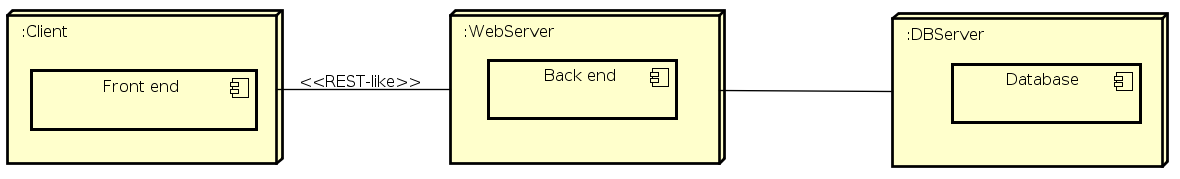
\includegraphics[width=0.8\textwidth]{res/sections/GeneralArchitecture.png}
\caption{Diagramma di deployment per l'architettura}
\end{figure}
L'architettura proposta segue il Design Pattern MVC. In particolare i ruoli di Model e Controller verranno implementati a livello di server, mentre il ruolo di View viene affidato al frontend. L'interfaccia tra le due componenti verrà gestita grazie ad un set di API disposto dal server REST: in questo modo si garantisce una totale indipendenza tra frontend e backend e sono possibili sviluppi futuri anche in altre piattaforme (ad esempio in app mobile) senza dover creare dei sistemi di integrazione ad-hoc. \\
Le tre macrocomponenti verranno descritte in dettaglio in seguito su questo documento.
\subsection{Interfaccia REST-like}
Il backend si basa su uno stile REST-like. Dal login al logout l'interfaccia di accesso ai dati può considerarsi a tutti gli effetti REST, ovvero con le seguenti caratteristiche:
\begin{itemize}
\item stato dell'applicazione e funzionalità divisi in risorse web;
\item ogni risorsa è unica e indirizzabile attraverso un URI (\textbf{U}niform \textbf{R}esource \textbf{I}dentifier);
\item tutte le risorse sono condivise come interfaccia uniforme per il trasferimento di stato tra client e risorse. Questo trasferimento consiste in:
\begin{itemize}
\item un insieme vincolato di operazioni ben definite;
\item un insieme vincolato di contenuti, opzionalmente supportato da codice a richiesta;
\item un protocollo:
\begin{itemize}
\item client-server;
\item privo di stato;
\item memorizzabile in cache;
\item a livelli.
\end{itemize}
\end{itemize}
\end{itemize}
REST utilizza il concetto di risorsa (aggregato di dati con un nome, l'URI, e una rappresentazione interna), sulla quale è possibile invocare operazioni CRUD (\textbf{C}reate, \textbf{R}ead, \textbf{U}pdate, \textbf{D}elete) con la seguente corrispondenza:
\begin{table}[H]
\centering
\label{CRUD}
\begin{tabular}{| >{\centering}p{3cm} | >{\centering}p{5cm} | >{\centering}p{6cm} |}
\hline
\textbf{Risorsa} & \textbf{URI della collection} \newline es. http://maas.com/users & \textbf{URI della risorsa} \newline es. http://maas.com/users/10 \tabularnewline \hline
\textbf{GET} & Fornisce informazioni sui membri della collection. & Fornisce una rappresentazione dell'elemento della collection indicato. \tabularnewline \hline
\textbf{PUT} & Non usata. & Sostituisce una rappresentazione dell'elemento della collection indicato. Se non esiste lo crea.  \tabularnewline \hline
\textbf{POST} & Crea un nuovo elemento della collection. La URI del nuovo elemento è generata automaticamente. & Non usato. \tabularnewline \hline
\textbf{DELETE} & Non usata. & Cancella l'elemento della collection indicato. \tabularnewline \hline
\end{tabular}
\caption{Tabella delle operazioni CRUD}
\end{table}
Per la rappresentazione dei dati si è scelto di utilizzare JSON perché si integra molto bene con i framework utilizzati e con il linguaggio JavaScript. Questo non è vero per XML (e\textbf{X}tensible \textbf{M}arkup \textbf{L}anguage) o CSV (\textbf{C}omma \textbf{S}eparated \textbf{V}alues), che richiederebbero librerie specifiche. Inoltre JSON è molto meno verboso e molto più flessibile di XML, e si adatta molto bene al dominio dell'applicazione.

\section{Backend}
\subsection{Formalismo utilizzato}
L'utilizzo del framework ExpressJS come base per il server ha evidenziato la necessità di regolamentare alcune convenzioni utilizzate. Queste convenzioni riguardano il formalismo utilizzato per la rappresentazione in quanto concetti come moduli, middlewares e first-class function non hanno una corrispondenza diretta nei diagrammi UML.
%I moduli verranno rappresentati come classi.

%% DA FINIRE E DEFINIRE CON MATTEO

\subsection{Descrizione generale}
L'implementazione scelta per il backend dell'applicazione è un server con architettura REST. Ciò implica che:
\begin{itemize}
\item l'applicazione renda disponibili le sue funzioni in veste di risorse web;
\item ogni risorsa resa disponibile è indirizzabile univocamente utilizzando un indirizzo URL;
\item l'interfaccia delle risorse deve essere uniforme e deve garantire un insieme ben definito di operazioni e una gestione priva di stato delle operazioni.
\end{itemize}

Tale architettura permette l'indipendenza completa tra backend e frontend, permettendo così a espansioni su altre piattaforme senza dover modificare il backend dell'applicazione.

L'architettura del backend segue il design patter MVC (\textbf{M}odel \textbf{V}iew \textbf{C}ontroller) per quanto concerne i ruoli di Model e Controller. 
Il ruolo di Controller tuttavia, non essendo implementato nativamente in Express, verrà implementato da uno stack di middleware come suggerito dal framework.
La parte View, invece, è rapprestata dal frontend, costituito da componenti definiti con React e disposti secondo l'architettura Flux.

\subsection{Descrizione dei package}
Il seguente diagramma mostra l'architettura generale del backend.
\begin{figure}[H]
\centering
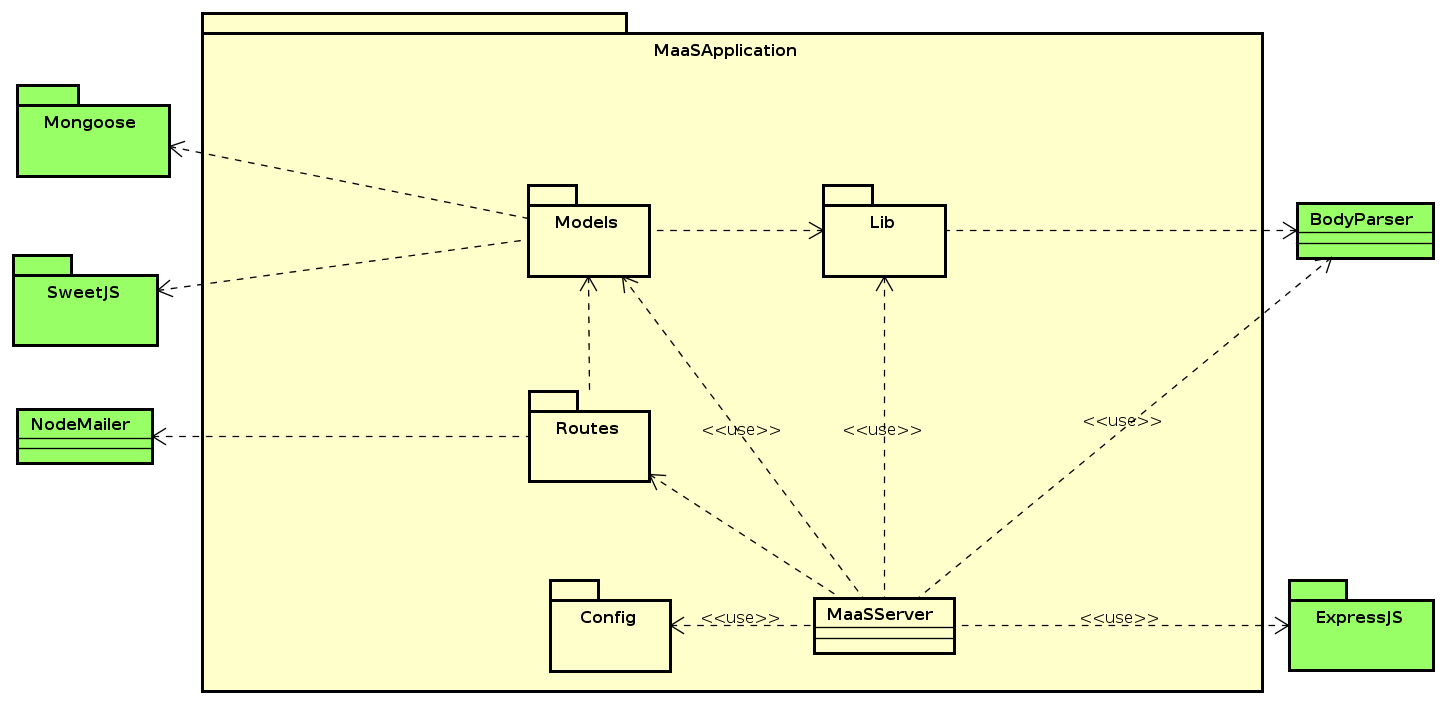
\includegraphics[width=0.8\textwidth]{res/sections/backend/generale.png}
\caption{Diagramma dei package}
\end{figure}

\subsubsection{Package MaaSApplication}
\paragraph*{Descrizione}
Package che racchiude tutta l'applicazione MaaS.

\paragraph*{Package contenuti}
\begin{itemize}
\item Models
\item Routes
\item Config
\item Lib
\end{itemize}

\paragraph*{Moduli contenuti}
\begin{itemize}
\item MaaSServer
\end{itemize}

\begin{figure}[H]
\centering
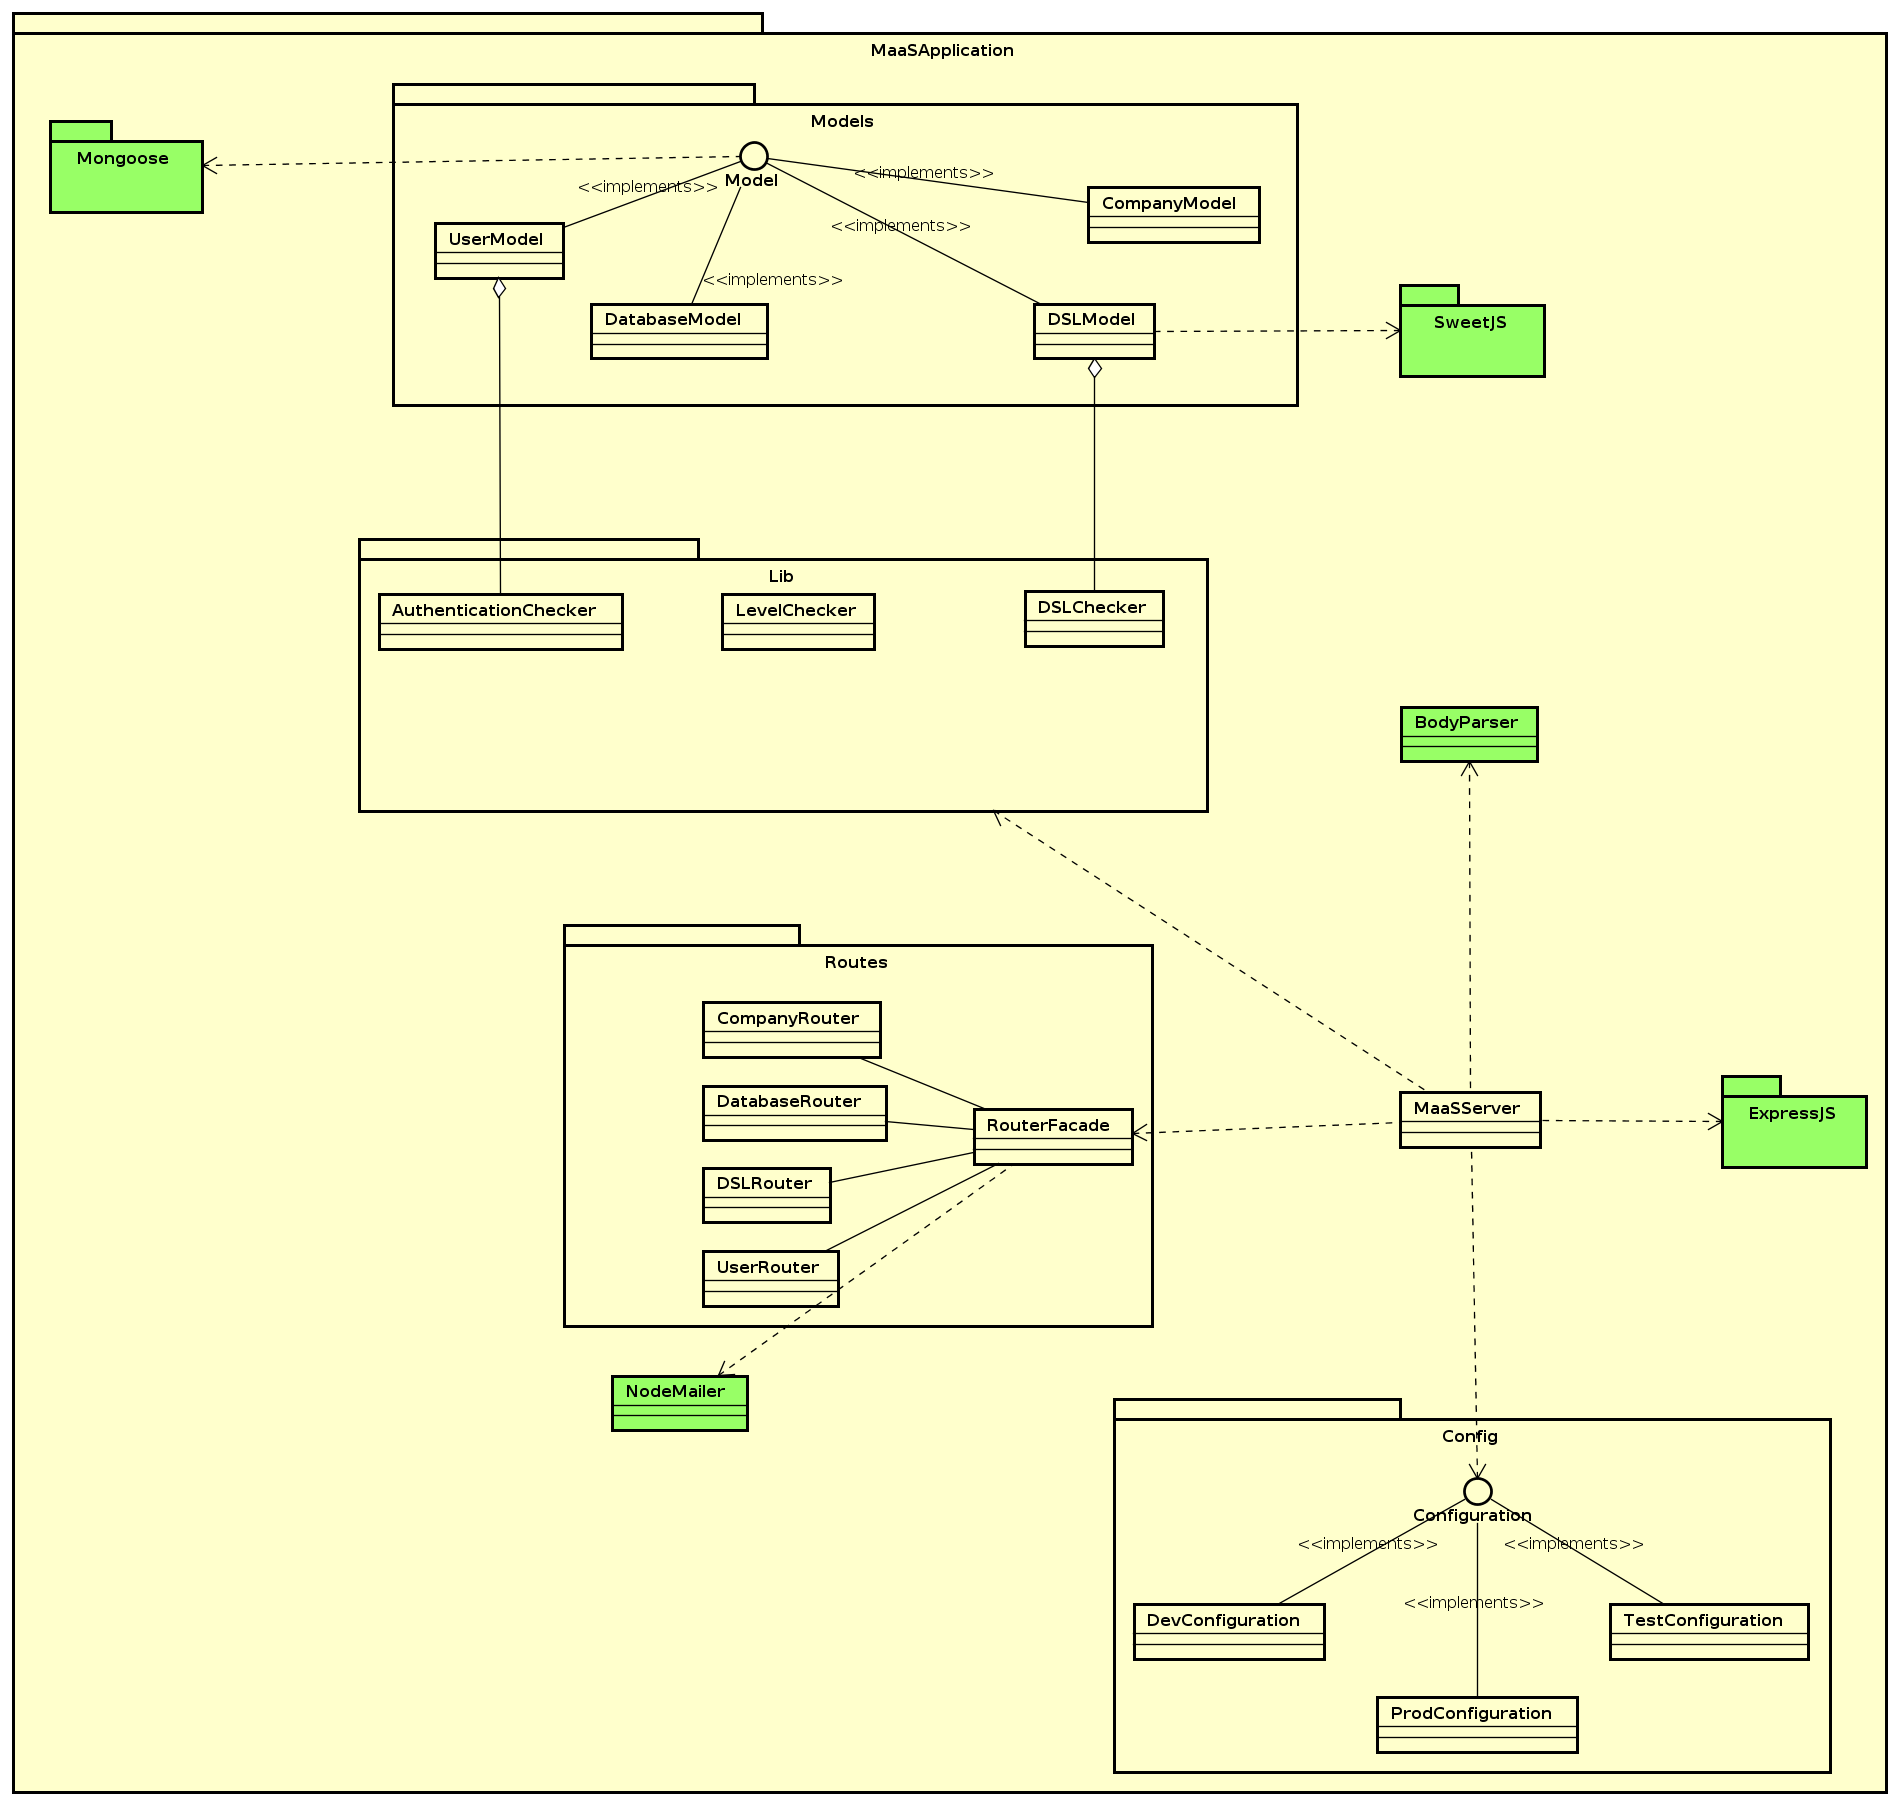
\includegraphics[width=0.8\textwidth]{res/sections/backend/collegamenti.png}
\caption{Diagramma dei package completo dei componenti per ciascun package}
\end{figure}

\subsection{Package Models}
\paragraph*{Descrizione}
Package che racchiude i moduli contenenti la business logic dell'applicazione. Ciascuno di questi moduli implementa un modello Mongoose e definisce i metodi con cui interagirvi (aggiungere, rimuovere e modificare i contenuti). \\
Rappresenta la parte M (Model) del design pattern MVC.

\paragraph*{Moduli contenuti}
\begin{itemize}
\item UserModel
\item DSLModel
\item CompanyModel
\item DatabaseModel
\end{itemize}

\paragraph*{Interfacce contenute}
\begin{itemize}
\item Model
\end{itemize}

\begin{figure}[H]
\centering
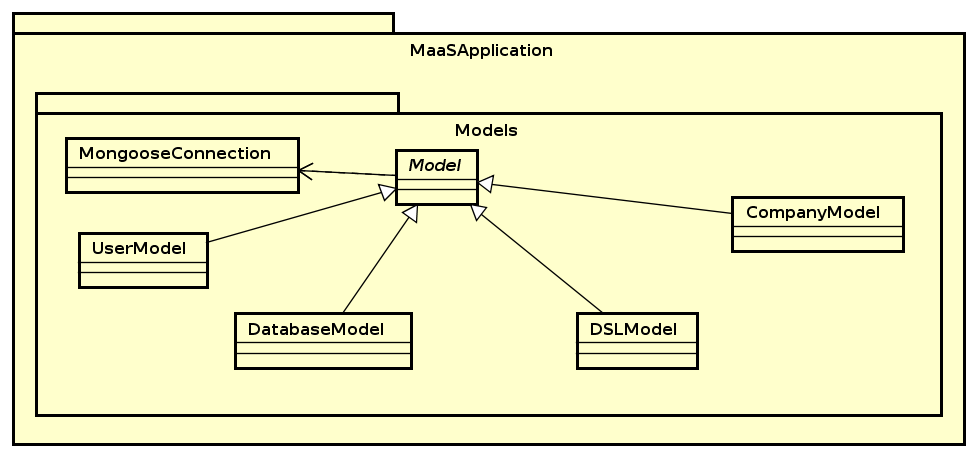
\includegraphics[width=0.8\textwidth]{res/sections/backend/models.png}
\caption{Diagramma delle classi del package Models}
\end{figure}

\subsubsection{UserModel}
\paragraph*{Descrizione}

Racchiude la business logic legata agli utenti. Viene implementato tramite Module pattern di Javascript. 

\paragraph*{Utilizzo}
Il modello viene utilizzato sia per la rappresentazione di un utente nell'applicazione, sia per l'autenticazione nel sistema.

\paragraph*{Relazioni con altri moduli}
\begin{itemize}
\item Mongoose
\item Mongoose-validator
\item Lib::AuthenticationChecker
\end{itemize}

\subsubsection{CompanyModel}
\paragraph*{Descrizione}
Racchiude la business logic legata alle Company. Viene implementato tramite Module pattern di Javascript. 

\paragraph*{Utilizzo}
Il modello rappresenta una Company nel sistema.

\paragraph*{Relazioni con altri moduli}
\begin{itemize}
\item Mongoose
\item Mongoose-validator
\end{itemize}

\paragraph{DatabaseModel}
\paragraph*{Descrizione}

Racchiude la business logic legata al collegamento con i database delle Company. Viene implementato tramite Module pattern di Javascript. 

\paragraph*{Utilizzo}
Il modello rappresenta la connessione ad un database aziendale di una company. Contiene i dati per effettuare l'accesso al database e il riferimento alle collections definite su tale database, permettendo così all'utente di poter definire per ciascuna collection la possibilità di interagirvi da parte di tutti i membri della propria Company o solo degli admin.

\paragraph*{Relazioni con altri moduli}
\begin{itemize}
\item Mongoose
\item Mongoose-validator
\end{itemize}

\paragraph{DSLModel}
\paragraph*{Descrizione}

Racchiude la business logic legata alle specifiche DSL. Viene implementato tramite Module pattern di Javascript. 

\paragraph*{Utilizzo}
Il modello viene utilizzato per la rappresentazione delle specifiche DSL. Contiene i dati di tali specifiche e le funzioni per poter estrarre i dati richiesti da una specifica DSL.

\paragraph*{Relazioni con altri moduli}
\begin{itemize}
\item Mongoose
\item Mongoose-validator
\item DSLChecker
\item DatabaseModel
\end{itemize}

\paragraph{Model}
\paragraph*{Descrizione}
Interfaccia comune a tutti i modelli usati da MaaS.

\paragraph*{Utilizzo}
Viene utilizzata come base per UserModel, CompanyModel, DSLModel e DatabaseModel.

\paragraph*{Relazione con altri moduli}
\begin{itemize}
\item Mongoose
\item UserModel
\item CompanyModel
\item DSLModel
\item DatabaseModel
\end{itemize}

\subsubsection{Package Routes}
\paragraph*{Descrizione}
Il package Routes contiene l'implementazione dei Router definiti da ExpressJS. Il package è costituito da una serie di moduli che implementano gli endpoint per le API.
I moduli vengono suddivisi in base al modello che utilizzano. Ciascuna route definita inoltre ha il compito di richiamare i middleware necessari.
La definizione delle API seguirà la descrizione riportata nella sezione apposita di questo documento.\\
Reppresenta la parte C (Controller) del design pattern MVC.

\paragraph*{Moduli contenuti}
\begin{itemize}
\item UserRouter
\item CompanyRouter
\item DSLRouter
\item DatabaseRouter
\item RouterFacade
\end{itemize}

\paragraph*{Interfacce contenute}
\begin{itemize}
\item Router
\end{itemize}

\begin{figure}[H]
\centering
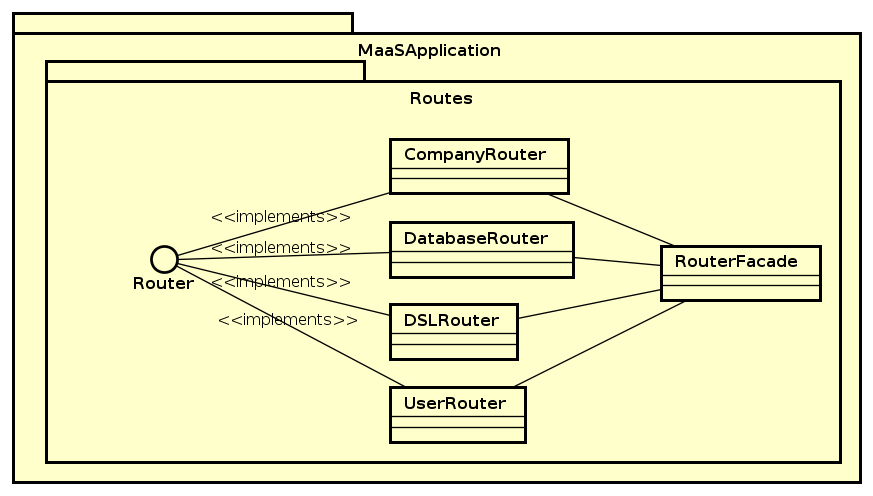
\includegraphics[width=0.8\textwidth]{res/sections/backend/routes.png}
\caption{Diagramma delle classi del package Routes}
\end{figure}

\paragraph{UserRouter}
\paragraph*{Descrizione}
Questo modulo contiene la definizione degli endpoint riguardanti gli utenti. 

\paragraph*{Relazione con altri moduli}
\begin{itemize}
\item AuthenticationChecker
\item UserModel
\end{itemize}

\paragraph{CompanyRouter}
\paragraph*{Descrizione}
Questo modulo contiene la definizione degli endpoint riguardanti le company.

\paragraph*{Relazione con altri moduli}
\begin{itemize}
\item AuthenticationChecker
\item CompanyModel
\end{itemize}

\paragraph{DSLRouter}
\paragraph*{Descrizione}
Questo modulo contiene la definizione degli endpoint riguardanti le specifiche DSL.

\paragraph*{Relazione con altri moduli}
\begin{itemize}
\item AuthenticationChecker
\item DSLModel
\end{itemize}

\paragraph{DatabaseRouter}
\paragraph*{Descrizione}
Questo modulo contiene la definizione degli endpoint riguardanti le connessioni ai database aziendali.

\paragraph*{Relazione con altri moduli}
\begin{itemize}
\item AuthenticationChecker
\item DatabaseModel
\end{itemize}

\paragraph{RouterFacade}
\paragraph*{Descrizione}
Oggetto che implementa il Facade Design Pattern. Tale oggetto incorpora tutti gli endpoint definiti dagli altri router.

\paragraph*{Relazione con altri moduli}
\begin{itemize}
\item AuthenticationChecker
\item UserRouter
\item CompanyRouter
\item DSLRouter
\item DatabaseRouter
\end{itemize}

\paragraph{Router}
\paragraph*{Descrizione}
Interfaccia comune ai router usati da MaaS.

\paragraph*{Utilizzo}
Viene utilizzata come base per UserRouter, CompanyRouter, DSLRouter e DatabaseRouter.

\paragraph*{Relazione con altri moduli}
\begin{itemize}
\item BodyParser
\item UserRouter
\item CompanyRouter
\item DSLRouter
\item DatabaseRouter
\end{itemize}

\subsubsection{Package Config}
\paragraph*{Descrizione}
Questo package contiene la classe Configuration che, in base alla variabile d'ambiente NODE\_ENV, restituisce l'oggetto contenente tutte le informazioni utili alla configurazione del server.

\paragraph*{Moduli contenuti}
\begin{itemize}
\item Configuration
\item DevConfiguration
\item TestConfiguration
\item ProdConfiguration
\end{itemize}

\paragraph*{Interfacce contenute}
\begin{itemize}
\item Configuration
\end{itemize}

\begin{figure}[H]
\centering
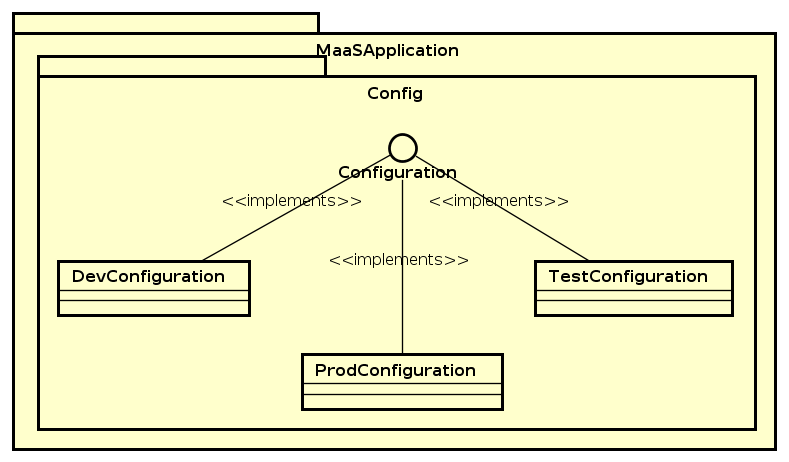
\includegraphics[width=0.8\textwidth]{res/sections/backend/config.png}
\caption{Diagramma delle classi del package Config}
\end{figure}

\paragraph{DevConfiguration}
\paragraph*{Descrizione}
Configurazione usata durante lo sviluppo.

\paragraph*{Utilizzo}
Viene utilizzata per configurare l'ambiente di lavoro durante lo sviluppo di MaaS.

\paragraph{TestConfiguration}
\paragraph*{Descrizione}
Configurazione usata durante il test.

\paragraph*{Utilizzo}
Viene utilizzata per configurare l'ambiente di lavoro durante il test di MaaS.

\paragraph{ProdConfiguration}
\paragraph*{Descrizione}
Configurazione usata per il rilascio.

\paragraph*{Utilizzo}
Viene utilizzata per configurare l'ambiente di lavoro per la consegna di MaaS.

\paragraph{Configuration}
\paragraph*{Descrizione}
Interfaccia comune alle configurazioni usate da MaaS.

\paragraph*{Utilizzo}
Viene utilizzata come base per DevConfiguration, TestConfiguration e ProdConfiguration.

\paragraph*{Relazione con altri moduli}
\begin{itemize}
\item MaaSServer
\end{itemize}

\subsubsection{Package Lib}
\paragraph*{Descrizione}
Questo package contiene tutti i moduli di supporto al sistema e i middlewares generici per ExpressJS.

\paragraph*{Moduli contenuti}
\begin{itemize}
\item LevelChecker
\item AuthenticationChecker
\item DSLChecker
\end{itemize}

\paragraph{Interfacce contenute}
\begin{itemize}
\item Middleware
\end{itemize}

\begin{figure}[H]
\centering
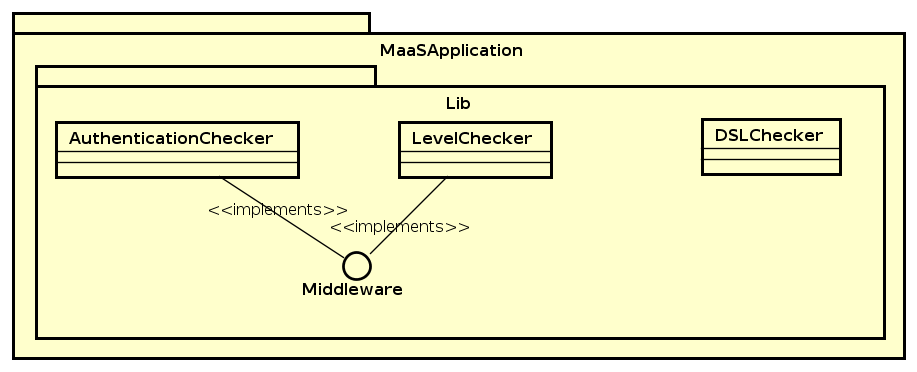
\includegraphics[width=0.8\textwidth]{res/sections/backend/lib.png}
\caption{Diagramma delle classi del package Lib}
\end{figure}

\paragraph{LevelChecker}
\paragraph*{Descrizione}
Middleware che si occupa di verificare se l'utente che effettua una richiesta al server ha i livelli minimi di accesso per poterla eseguire.

\paragraph*{Utilizzo}
Viene utilizzato nelle routes in cui deve essere garantito un livello utente minimo di accesso per portare a termine la richiesta.

\paragraph*{Relazione con altri moduli}
\begin{itemize}
\item Router
\end{itemize}

\paragraph{AuthenticationChecker}
\paragraph*{Descrizione}
Modulo che definisce due middleware: uno per effettuare il login, l'altro per l'autenticazione di una richiesta.

\paragraph*{Utilizzo}
Questo modulo viene utilizzato per definire l'endpoint per effettuare il login all'applicazione e offre il middleware che permette di autenticare le richieste. Tale middleware si occuperà di estrarre il token dalle richieste, verificarne la correttezza e aggiungere l'utente verificato nella richiesta per i prossimi middleware.

\paragraph*{Relazione con altri moduli}
\begin{itemize}
\item Router
\end{itemize}

\paragraph{DSLChecker}
\paragraph*{Descrizione}
Modulo che verifica la correttezza sintattica e di contenuto di una specifica DSL.

\paragraph*{Utilizzo}
Questo modulo viene richiamato in DSLModel per verificare che la specifica DSL che viene salvata o modificata sia valida per l'esecuzione.

\paragraph*{Relazione con altri moduli}
\begin{itemize}
\item DSLModel
\end{itemize}

\paragraph{Middleware}
\paragraph*{Descrizione}
Interfaccia comune ai middlware usati da MaaS.

\paragraph*{Utilizzo}
Viene utilizzata come base per AuthenticationChecker e per LevelChecker.

\paragraph*{Relazione con altri moduli}
\begin{itemize}
\item BodyParser
\item AuthenticationChecker
\item LevelChecker
\end{itemize}

\subsubsection{Modulo MaaSServer}
\paragraph*{Descrizione}
Modulo principale dell'applicazione.

\paragraph*{Utilizzo}
Viene 

\paragraph*{Relazione con altri moduli}
\begin{itemize}
\item Config
\item RouterFacade
\item BodyParser
\end{itemize}

\paragraph*{Relazione con altri package}
\begin{itemize}
\item Lib
\item ExpressJS
\end{itemize}

\subsubsection{Moduli integrati}
\paragraph{BodyParser}
\paragraph*{Descrizione}
?????????????????

\paragraph*{Utilizzo}
??????????????????

\paragraph{NodeMailer}
\paragraph*{Descrizione}
Permette di inviare delle email.

\paragraph*{Utilizzo}
È usato per inviare email agli utenti di MaaS.

\subsubsection{Framework integrati}
\paragraph{SweetJS}
\paragraph*{Descrizione}
?????????????????

\paragraph*{Utilizzo}
??????????????????

\paragraph{ExpressJS}
\paragraph*{Descrizione}
Framework per la creazione e la gestione di API REST.

\paragraph*{Utilizzo}
Utilizzato come base per la struttura del server.

\paragraph{Mongoose}
\paragraph*{Descrizione}
Framework per interfacciarsi con MongoDB.

\paragraph*{Utilizzo}
Utilizzato per la gestione dei dati su database MongoDB.

\subsection{API REST}
\subsubsection{Comunicazione tra client e server}
Per la creazione del back end di MaaS si è deciso di utilizzare Node.js e, in particolare, il framework ExpressJS, che permette la creazione semplificata di server REST. Il lato back end sarà quindi costituito da un insieme di API protette da strati diversi di sicurezza. \\
Ciascuna API del webserver fornirà una risposta in formato JSON per permettere la fruizione delle informazioni. Fornirà nello stesso formato anche gli eventuali messaggi di errore generati nel corpo dei metodi del server. Tali messaggi di errore saranno così composti: 
\begin{verbatim}
{
    "code":     [Codice definito nel protocollo HTTP, che identifica univocamente
                 la tipologia del problema]
    "message":  [Messaggio che definisce in dettaglio la tipologia dell'errore]
    ["data":   [Opzionale, trasporta i dati in cui si è verificato l'errore]]
}
\end{verbatim}
I codici di errore saranno del tipo 4xx (client error, la richiesta è sintatticamente scorretta o non può essere soddisfatta) o 5xx (server error, il server ha fallito nel soddisfare una richiesta apparentemente valida).
\subsubsection{Sicurezza}
Gli accessi alle API avranno 2 livelli di sicurezza. \\
Il primo livello è rappresentato dall'autenticazione: un utente non autenticato riceverà un errore se richiede una API protetta. Verrà implementato con l'utilizzo di PassportJS, un middleware per ExpressJS che permette l'autenticazione di utenti nel sistema. In particolare verrà utilizzata la strategia passport-local per l'accesso al server, cioè le credenziali dell'utente risiederanno nel database locale. \\
Il secondo livello è definito in base al ruolo di appartenenza di un utente. Si occuperà di controllare i permessi assegnati ad un utente autenticato e di verificare la possibilità che possa o meno interagire con la risorsa richiesta. \\
I ruoli utente ammessi nell'applicazione sono: 
\begin{itemize}
\item \textbf{GUEST};
\item \textbf{MEMBER};
\item \textbf{ADMIN};
\item \textbf{OWNER};
\item \textbf{SUPERADMIN}.
\end{itemize}
Per il ruolo di SUPERADMIN è abilititato un set di API per la gestione dell'intera applicazione. Tali API non sono accessibili agli utenti con altri ruoli.
\newpage
\subsubsection{Scenari di accesso negato}
Di seguito verranno rappresentati scenari corrispondenti ad una negazione di accesso per ruolo non conforme alle attese o per errore nel login.
\paragraph{Errore di autenticazione}  \mbox{} \\
\textbf{Descrizione:} L'utente non autenticato cerca di accedere a MaaS, ma la procedura di login rileva un errore nelle credenziali inserite.
\begin{figure}[H]
\centering
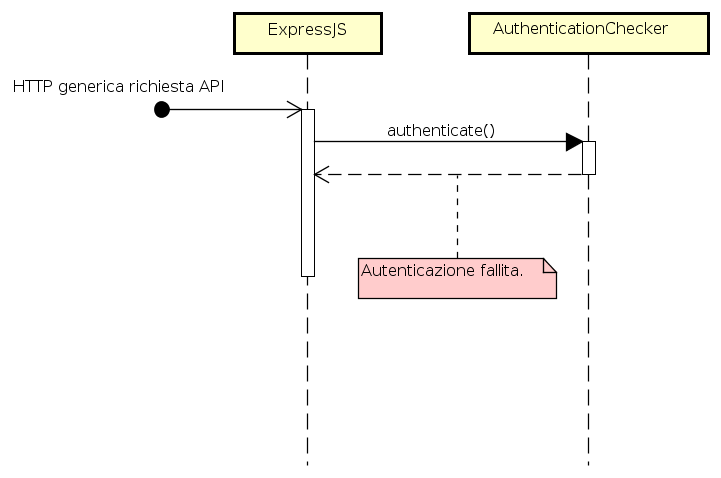
\includegraphics[width=0.8\textwidth]{res/sections/backend/sequence/autenticazioneFallita.png}
\caption{Autenticazione fallita}
\end{figure}
\paragraph{Livello minimo: MEMBER} \mbox{} \\
\textbf{Descrizione:} Tentativo di accesso ad una risorsa visibile solo a utenti con ruolo almeno MEMBER da parte di un utente GUEST.
\begin{figure}[H]
\centering
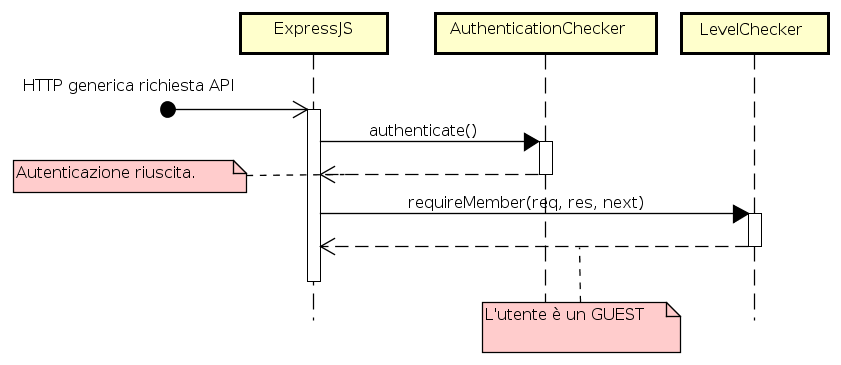
\includegraphics[width=0.8\textwidth]{res/sections/backend/sequence/requireMemberFallita.png}
\caption{Livello minimo MEMBER}
\end{figure}
\paragraph{Livello minimo: ADMIN} \mbox{} \\
\textbf{Descrizione:} Tentativo di accesso ad una risorsa visibile solo a utenti con ruolo almeno ADMIN da parte di un utente GUEST o MEMBER.
\begin{figure}[H]
\centering
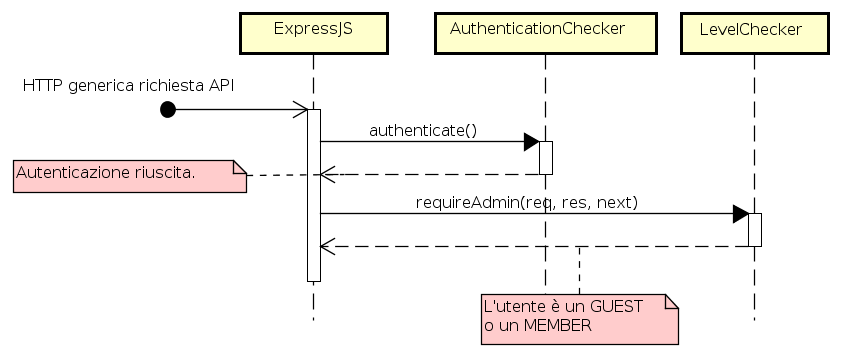
\includegraphics[width=0.8\textwidth]{res/sections/backend/sequence/requireAdminFallita.png}
\caption{Livello minimo ADMIN}
\end{figure}
\paragraph{Livello minimo: OWNER}  \mbox{} \\
\textbf{Descrizione:} Tentativo di accesso ad una risorsa visibile solo a utenti con ruolo almeno OWNER da parte di un utente GUEST, MEMBER o ADMIN.
\begin{figure}[H]
\centering
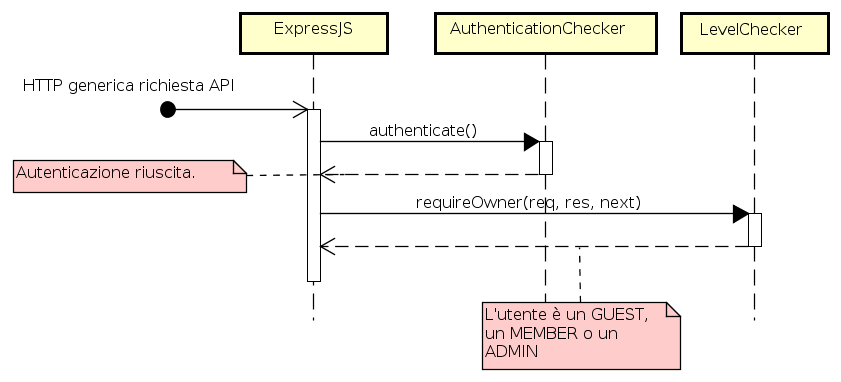
\includegraphics[width=0.8\textwidth]{res/sections/backend/sequence/requireOwnerFallita.png}
\caption{Livello minimo OWNER}
\end{figure}
\paragraph{Livello minimo: SUPERADMIN}  \mbox{} \\
\textbf{Descrizione:} Tentativo di accesso ad una risorsa accedibile solo da un SUPERADMIN da parte di un generico utente di MaaS.
\begin{figure}[H]
\centering
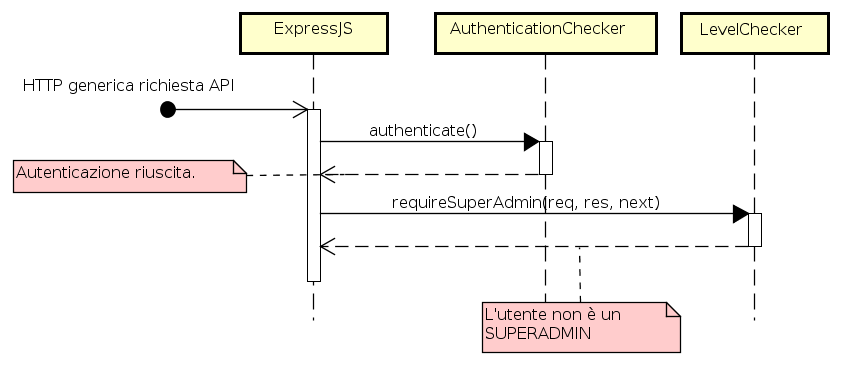
\includegraphics[width=0.8\textwidth]{res/sections/backend/sequence/requireSuperAdminFallita.png}
\caption{Livello minimo SUPERADMIN}
\end{figure}
\newpage
\subsection{API REST}
Di seguito sono descritte le API REST esposte dal server di MaaS. Si suppone che l'utente che richiede l'accesso alla risorsa descritta abbia i permessi necessari (ovvero che sia autenticato e che il suo ruolo sia conforme a quanto indicato). Qualora questo non fosse vero si ricadrebbe in uno degli scenari esposti precedentemente.
\subsubsection{Senza autenticazione}
\paragraph{Login}\mbox{}\\
\textbf{Tipologia:} POST \\
\textbf{API:} /api/login \\
\textbf{Descrizione:} Necessita di una richiesta con body contenente email e password dell'utente. \\
\textbf{Scenario:} 
\begin{figure}[H]
\centering
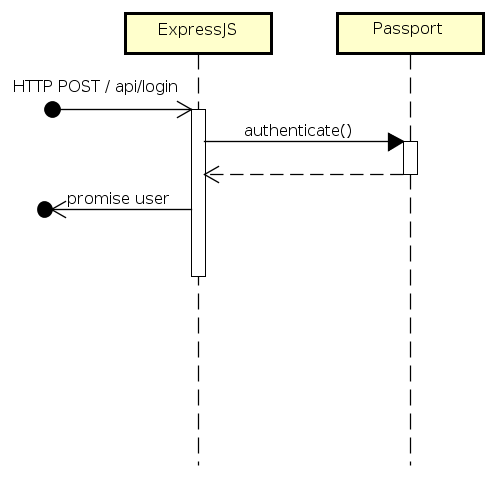
\includegraphics[width=0.8\textwidth]{res/sections/backend/sequence/(POST)login.png}
\caption{Scenario del login}
\end{figure}

\newpage
\paragraph{Registrazione}\mbox{}\\
\textbf{Tipologia:} POST \\
\textbf{API:} /api/register/:unique\_code \\
\textbf{Descrizione:} Metodo per la creazione di un utente invitato da una company. Necessita di una richiesta con body contenete le informazioni per la creazione completa di un utente \\
\textbf{Scenario:} 
\begin{figure}[H]
\centering
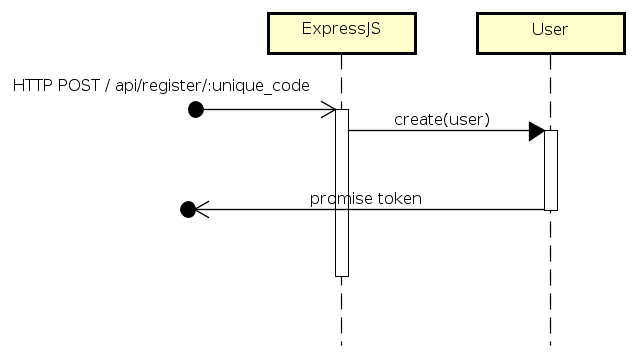
\includegraphics[width=0.8\textwidth]{res/sections/backend/sequence/(POST)register.png}
\caption{Scenario della registrazione}
\end{figure}

\newpage
\paragraph{Creazione Company}\mbox{}\\
\textbf{Tipologia:} POST \\
\textbf{API:} /api/companies \\
\textbf{Descrizione:} Necessita di una richiesta con body contenente le informazioni relative alla company e alla creazione del profilo del suo Owner. \\
\textbf{Scenario:} 
\begin{figure}[H]
\centering
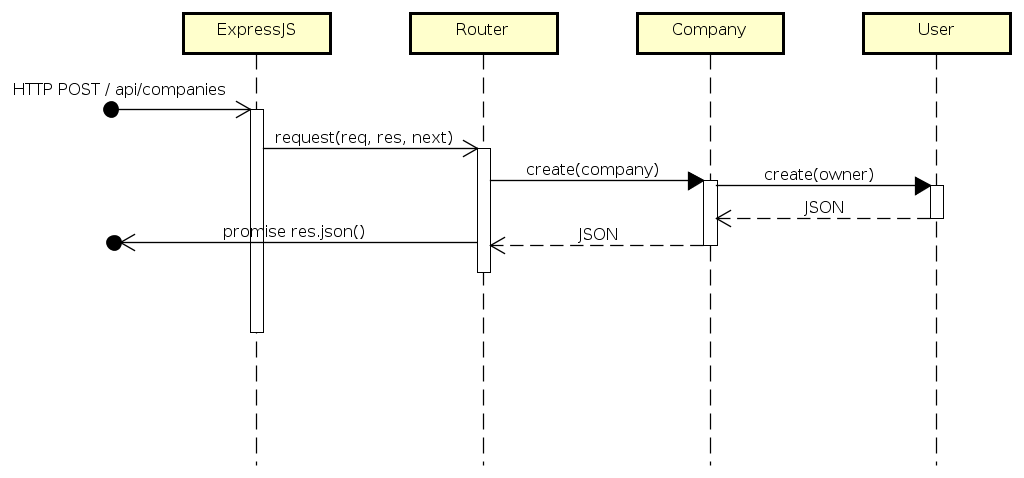
\includegraphics[width=0.8\textwidth]{res/sections/backend/sequence/(POST)company.png}
\caption{Scenario della creazione company}
\end{figure}

\newpage
\subsubsection{User}
\paragraph{Utenti di una company}\mbox{}\\
\textbf{Tipologia:} GET \\
\textbf{API:} /api/companies/:company\_id/users \\
\textbf{Livello di accesso minimo:} MEMBER \\
\textbf{Descrizione:} Ritorna un array di JSON contenenti i profili degli utenti della company. \\
\textbf{Scenario:} 
\begin{figure}[H]
\centering
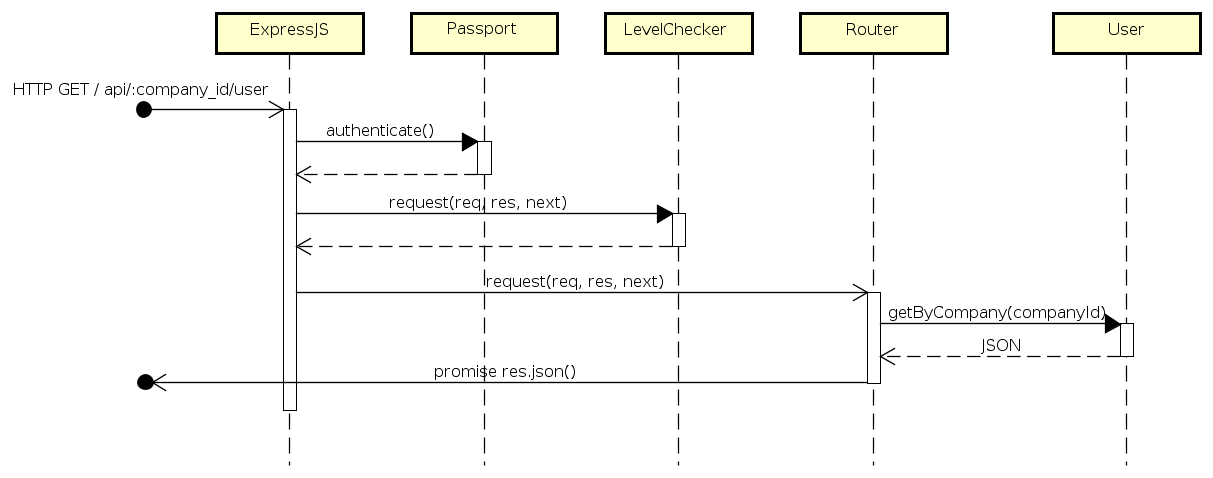
\includegraphics[width=0.8\textwidth]{res/sections/backend/sequence/(GET)user.png}
\caption{Scenario della ricerca utenti di una company specifica}
\end{figure}

\newpage
\paragraph{Inserimento utente}\mbox{}\\
\textbf{Tipologia:} POST \\
\textbf{API:} /api/companies/:company\_id/users \\
\textbf{Livello di accesso minimo:} OWNER \\
\textbf{Descrizione:} Necessita di una richiesta con body contenente l'email e il livello di accesso dell'utente.\\
\textbf{Scenario:} 
\begin{figure}[H]
\centering
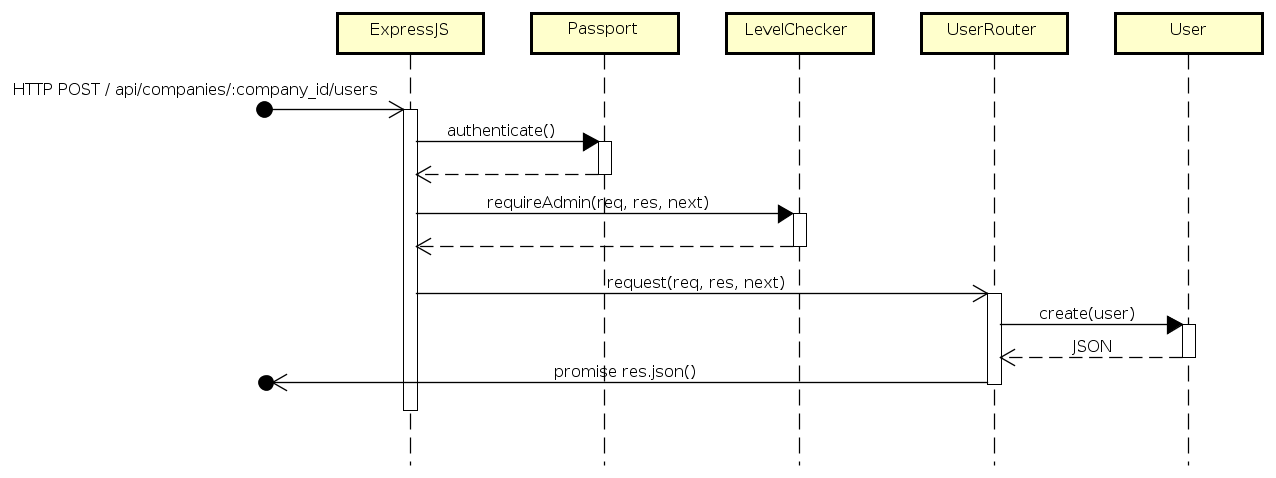
\includegraphics[width=0.8\textwidth]{res/sections/backend/sequence/(POST)user.png}
\caption{Scenario dell'inserimento utente in una company}
\end{figure}

\newpage
\paragraph{Aggiornamento delle credenziali utente}\mbox{}\\
\textbf{Tipologia:} PUT \\
\textbf{API:} /api/companies/:company\_id/users/:user\_id/credentials \\
\textbf{Livello di accesso minimo:} GUEST \\
\textbf{Descrizione:} Metodo per la modifica delle credenziali di accesso di un utente. Un utente ha il permesso di cambiare solo le proprie credenziali. \\
\textbf{Scenario:} 
\begin{figure}[H]
\centering
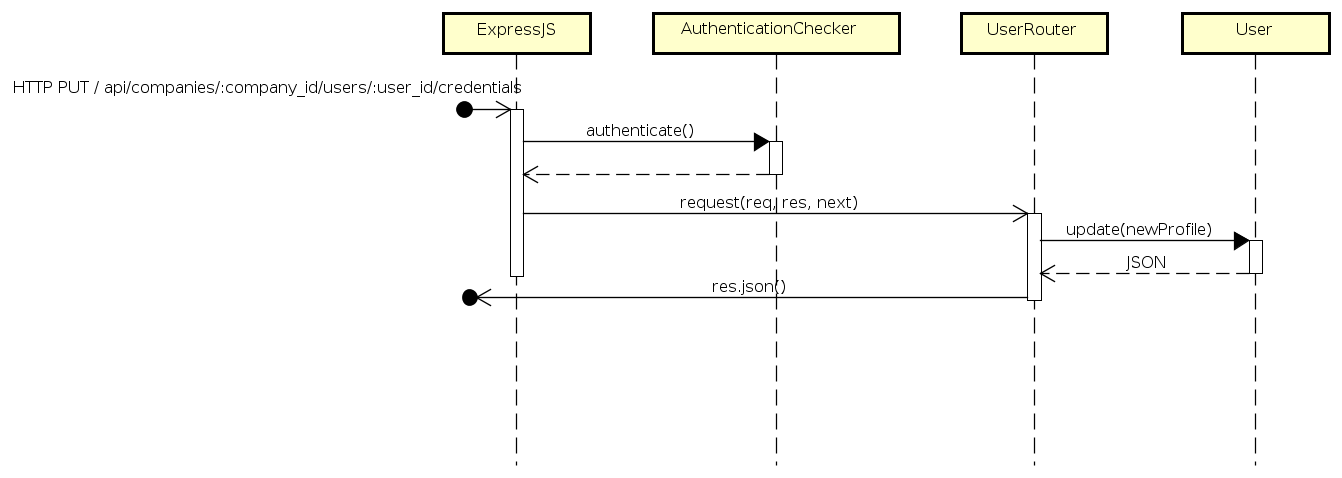
\includegraphics[width=0.8\textwidth]{res/sections/backend/sequence/(PUT)credenzialiUtente.png}
\caption{Scenario dell'aggiornamento delle credenziali di un utente}
\end{figure}

\newpage
\paragraph{Cancellazione utente}\mbox{}\\
\textbf{Tipologia:} DELETE \\
\textbf{API:} /api/companies/:company\_id/users/:user\_id \\
\textbf{Livello di accesso minimo:} OWNER \\
\textbf{Descrizione:} Ritorna un messaggio di conferma dell'avvenuta cancellazione. \\
\textbf{Scenario:} 
\begin{figure}[H]
\centering
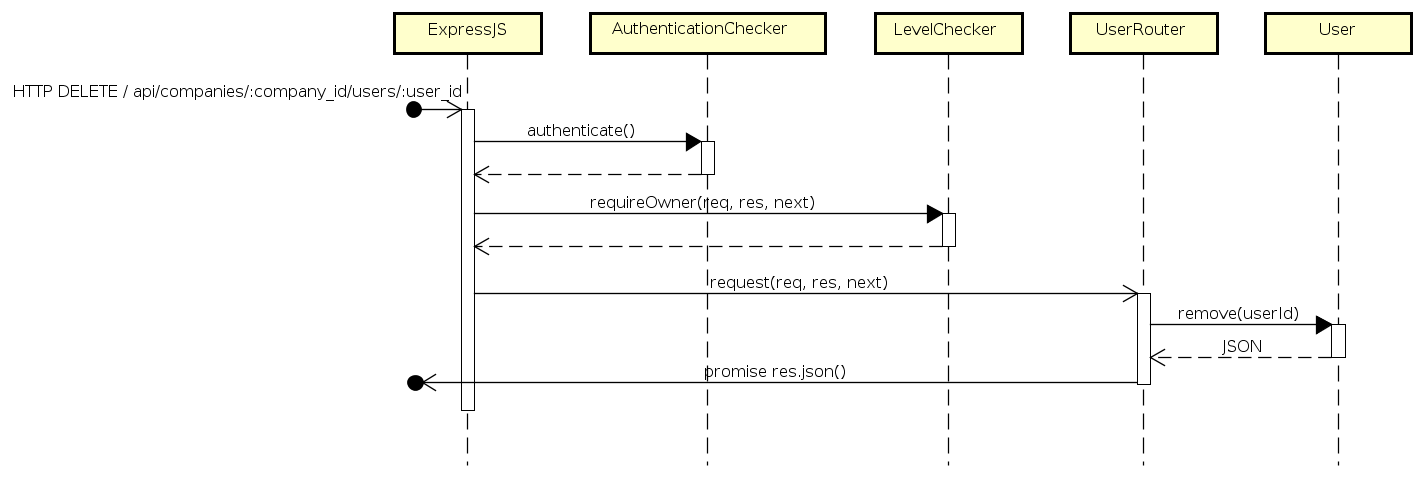
\includegraphics[width=0.8\textwidth]{res/sections/backend/sequence/(DELETE)user.png}
\caption{Scenario della cancellazione utente da una company}
\end{figure}

\newpage
\subsubsection{Company}
\paragraph{Dati di una company}\mbox{}\\
\textbf{Tipologia:} GET \\
\textbf{API:} /api/companies/:company\_id/ \\
\textbf{Livello di accesso minimo:} GUEST \\
\textbf{Descrizione:} Ritorna le informazioni generali di una company \\
\textbf{Scenario:} 
\begin{figure}[H]
\centering
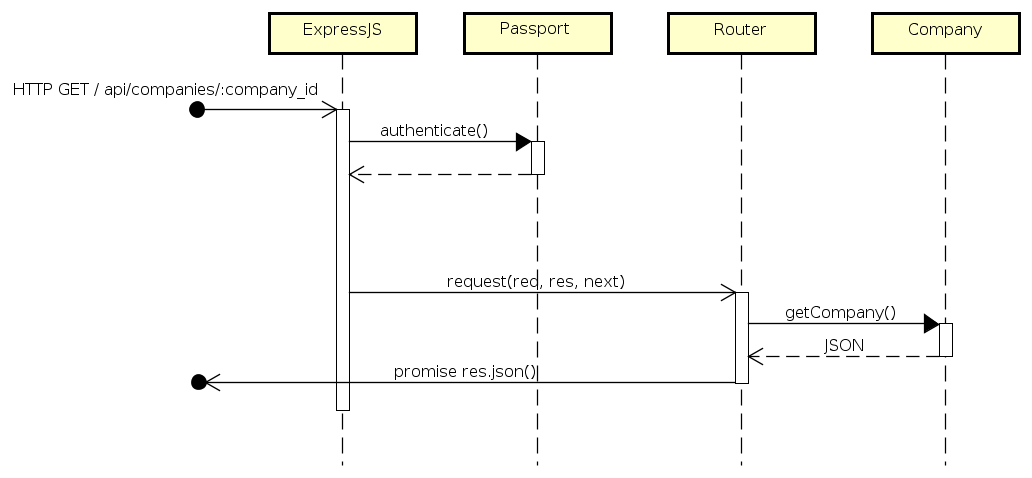
\includegraphics[width=0.8\textwidth]{res/sections/backend/sequence/(GET)company.png}
\caption{Scenario di ottenimento dei dati di una company}
\end{figure}

\newpage
\paragraph{Aggiornamento dei dati di una company}\mbox{}\\
\textbf{Tipologia:} PUT \\
\textbf{API:} /api/companies/:company\_id/ \\
\textbf{Livello di accesso minimo:} ADMIN \\
\textbf{Descrizione:} Necessita di una richiesta con body contenente le modifiche da apportare ai dati della company. \\
\textbf{Scenario:} 
\begin{figure}[H]
\centering
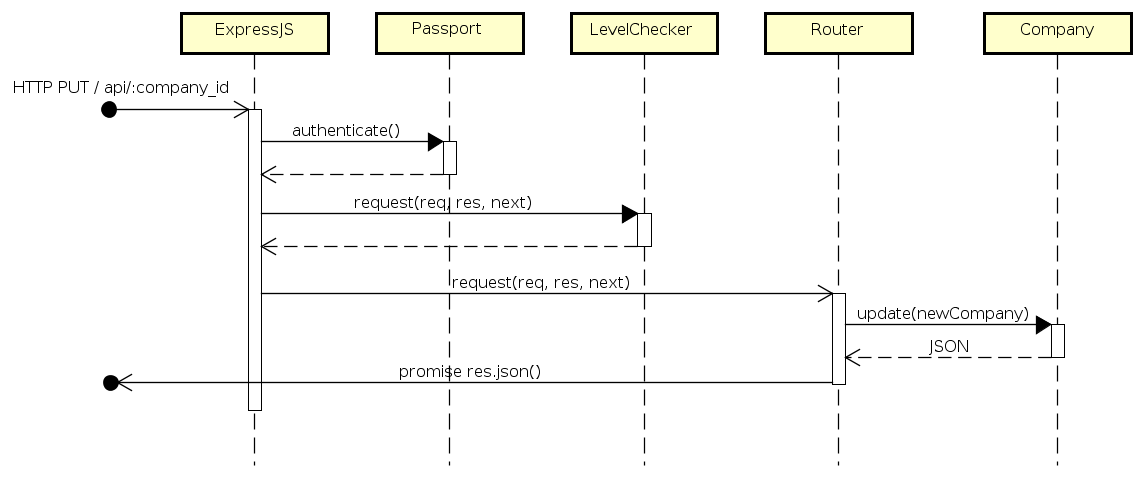
\includegraphics[width=0.8\textwidth]{res/sections/backend/sequence/(PUT)company.png}
\caption{Scenario dell'aggiornamento dei dati di una company}
\end{figure}

\newpage
\paragraph{Cancellazione di una company}\mbox{}\\
\textbf{Tipologia:} DELETE \\
\textbf{API:} /api/companies/:company\_id/ \\
\textbf{Livello di accesso minimo:} OWNER \\
\textbf{Descrizione:} Ritorna un messaggio di avvenuta cancellazione. \\
\textbf{Scenario:} 
\begin{figure}[H]
\centering
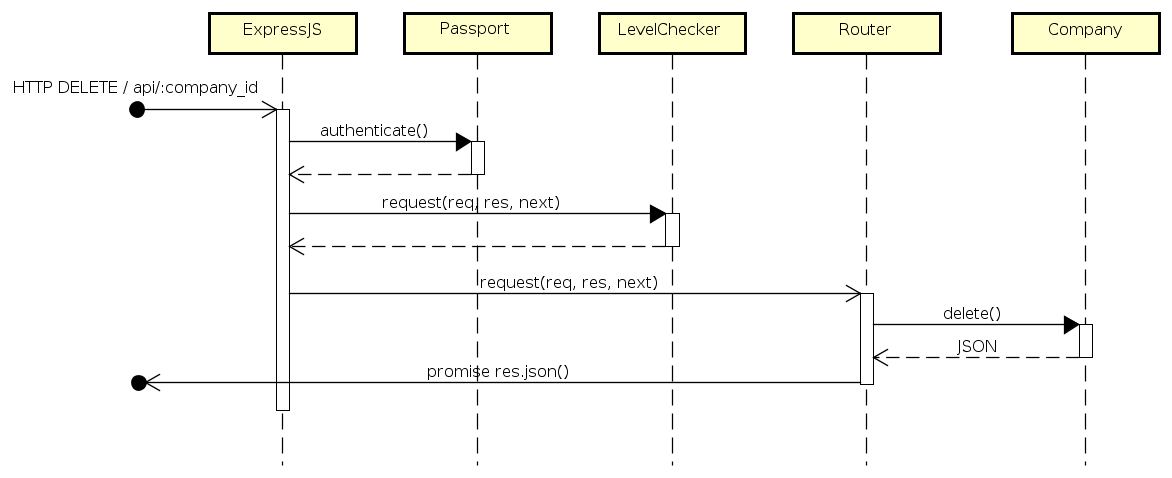
\includegraphics[width=0.8\textwidth]{res/sections/backend/sequence/(DELETE)company.png}
\caption{Scenario della cancellazione di una company}
\end{figure}

\newpage
\subsubsection{DSL}
\paragraph{Elenco delle specifiche DSL}\mbox{}\\
\textbf{Tipologia:} GET \\
\textbf{API:} /api/companies/:company\_id/DSLs \\
\textbf{Livello di accesso minimo:} GUEST \\
\textbf{Descrizione:} Ritorna un array contenente le specifiche DSL alle quali l'utente ha accesso in formato JSON. \\
\textbf{Scenario:} 
\begin{figure}[H]
\centering
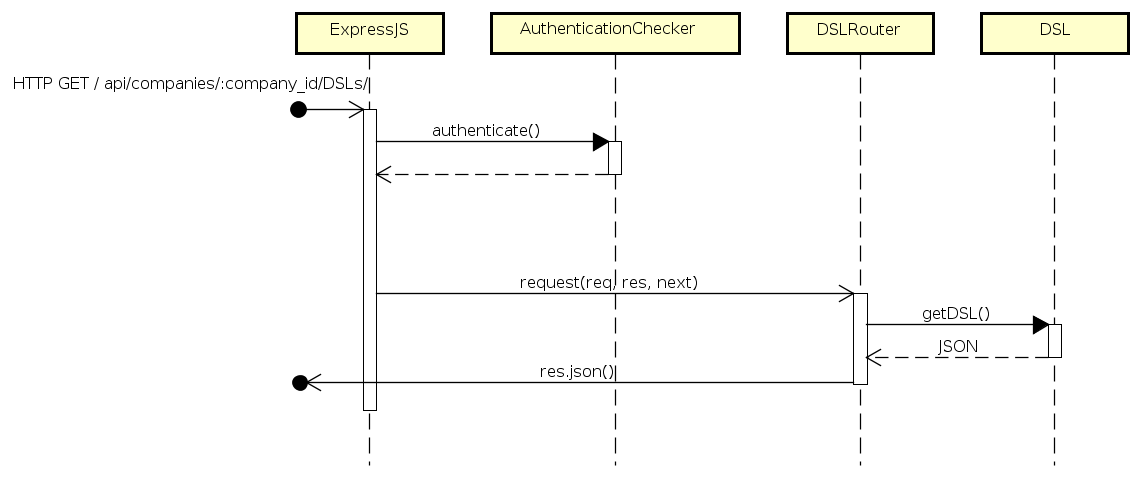
\includegraphics[width=0.8\textwidth]{res/sections/backend/sequence/(GET)dsl.png}
\caption{Scenario dell'elenco delle specifiche DSL}
\end{figure}

\newpage
\paragraph{Lettura del codice di una specifica DSL}\mbox{}\\
\textbf{Tipologia:} GET \\
\textbf{API:} /api/companies/:company\_id/DSLs/:dsl\_id \\
\textbf{Livello di accesso minimo:} MEMBER \\
\textbf{Descrizione:} Ritorna il codice della specifica DSL richiesta in formato JSON. \\
\textbf{Scenario:} 
\begin{figure}[H]
\centering
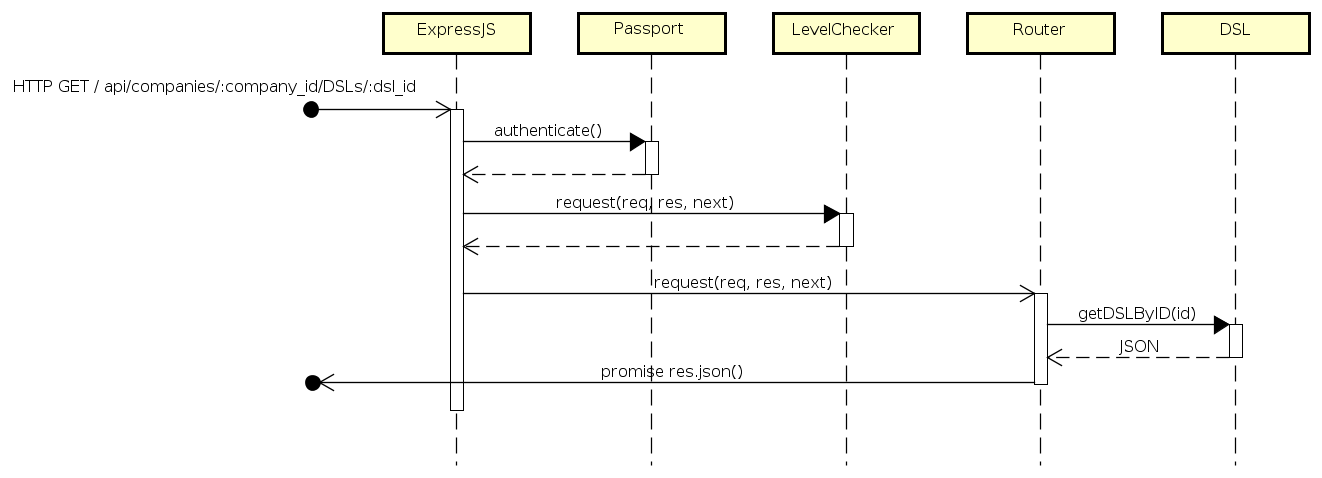
\includegraphics[width=0.8\textwidth]{res/sections/backend/sequence/(GET)dslByID.png}
\caption{Scenario della lettura del codice di una specifica DSL}
\end{figure}

\newpage
\paragraph{Aggiunta di una specifica DSL}\mbox{}\\
\textbf{Tipologia:} POST \\
\textbf{API:} /api/companies/:company\_id/DSLs \\
\textbf{Livello di accesso minimo:} MEMBER \\
\textbf{Descrizione:} Necessita di una richiesta con body contenente i dati necessari alla creazione della DSL. \\
\textbf{Scenario:} 
\begin{figure}[H]
\centering
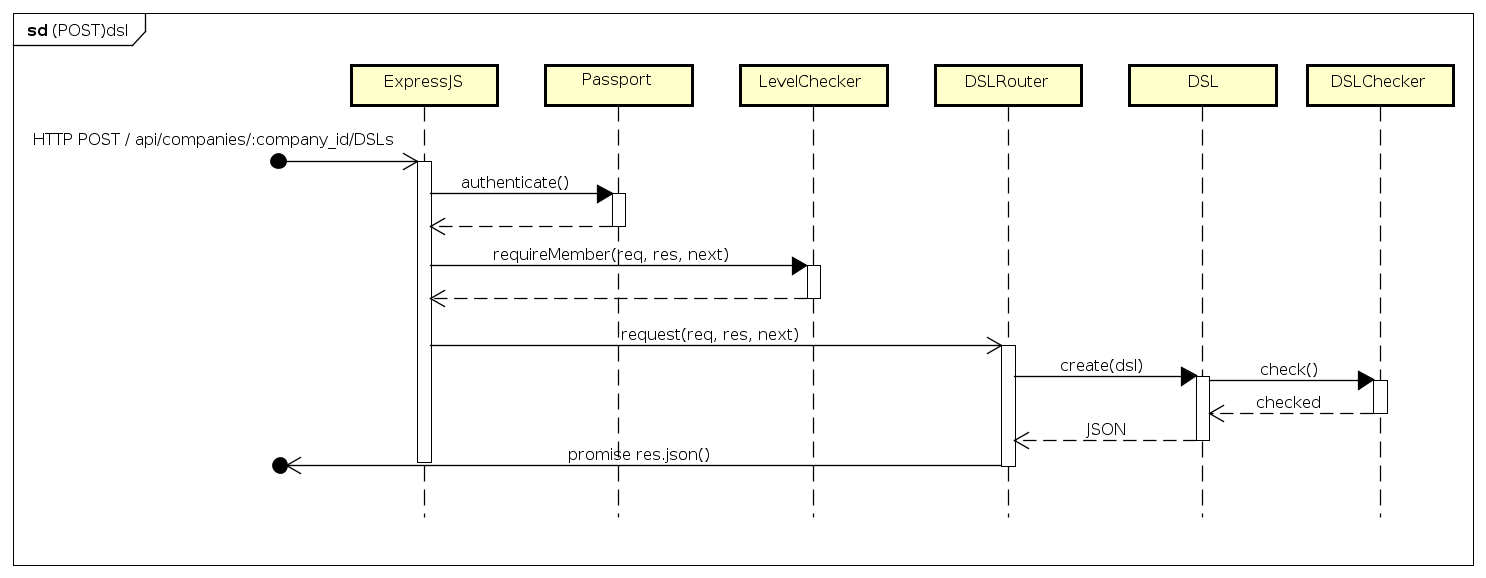
\includegraphics[width=0.8\textwidth]{res/sections/backend/sequence/(POST)dsl.png}
\caption{Scenario della creazione di una specifica DSL}
\end{figure}

\newpage
\paragraph{Aggiornamento del codice di una specifica DSL}\mbox{}\\
\textbf{Tipologia:} PUT \\
\textbf{API:} /api/companies/:company\_id/DSLs/:dsl\_id \\
\textbf{Livello di accesso minimo:} MEMBER \\
\textbf{Descrizione:} Necessita di una richiesta con body contenente i dati necessari alla modifica della DSL specificata da dsl\_id. \\
\textbf{Scenario:}
\begin{figure}[H]
\centering
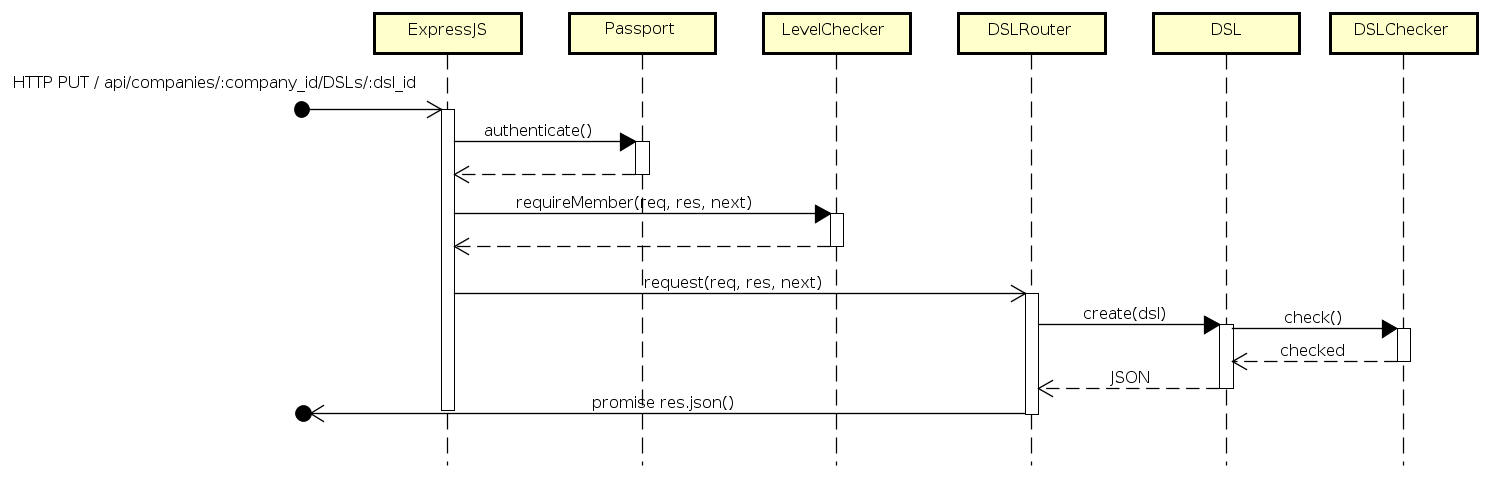
\includegraphics[width=0.8\textwidth]{res/sections/backend/sequence/(PUT)dsl.png}
\caption{Scenario dell'aggiornamento del codice di una specifica DSL}
\end{figure}

\newpage
\paragraph{Cancellazione di una specifica DSL}\mbox{}\\
\textbf{Tipologia:} DELETE \\
\textbf{API:} /api/companies/:company\_id/DSLs/:dsl\_id \\
\textbf{Livello di accesso minimo:} MEMBER \\
\textbf{Descrizione:} Ritorna un messaggio in formato JSON di avvenuta cancellazione. \\
\textbf{Scenario:} 
\begin{figure}[H]
\centering
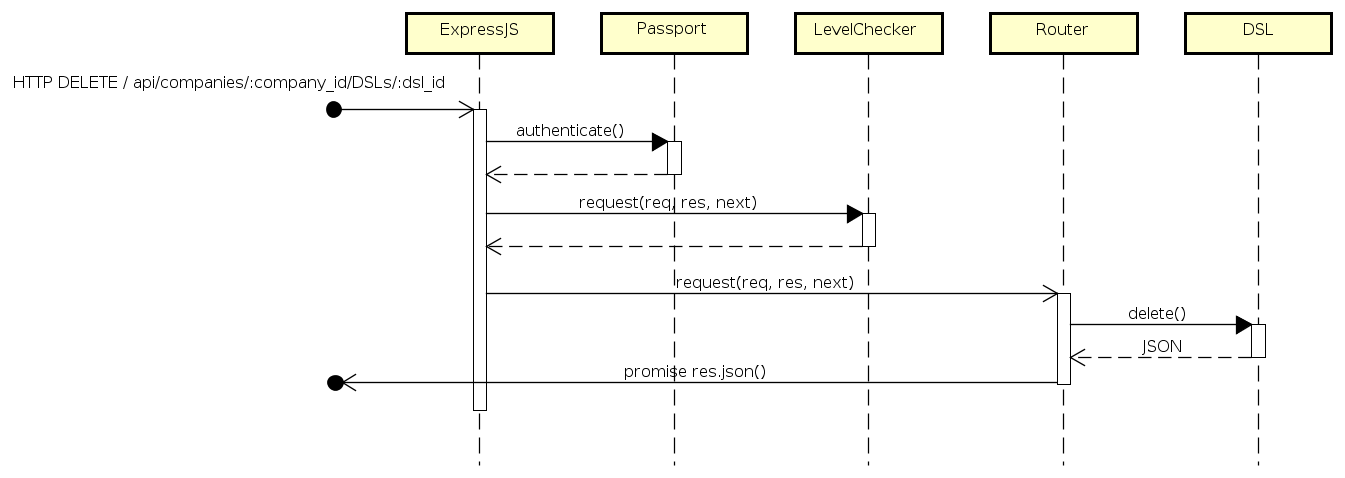
\includegraphics[width=0.8\textwidth]{res/sections/backend/sequence/(DELETE)dsl.png}
\caption{Scenario della cancellazione di una specifica DSL}
\end{figure}

\newpage
\paragraph{Ottenimento della dashboard di un utente}\mbox{}\\
\textbf{Tipologia:} GET \\
\textbf{API:} /api/companies/:company\_id/users/:user\_id/dashboard \\
\textbf{Livello di accesso minimo:} GUEST \\
\textbf{Descrizione:} Ritorna la dashboard di un utente definita da una DSL. \\
\textbf{Scenario:}  
\begin{figure}[H]
\centering
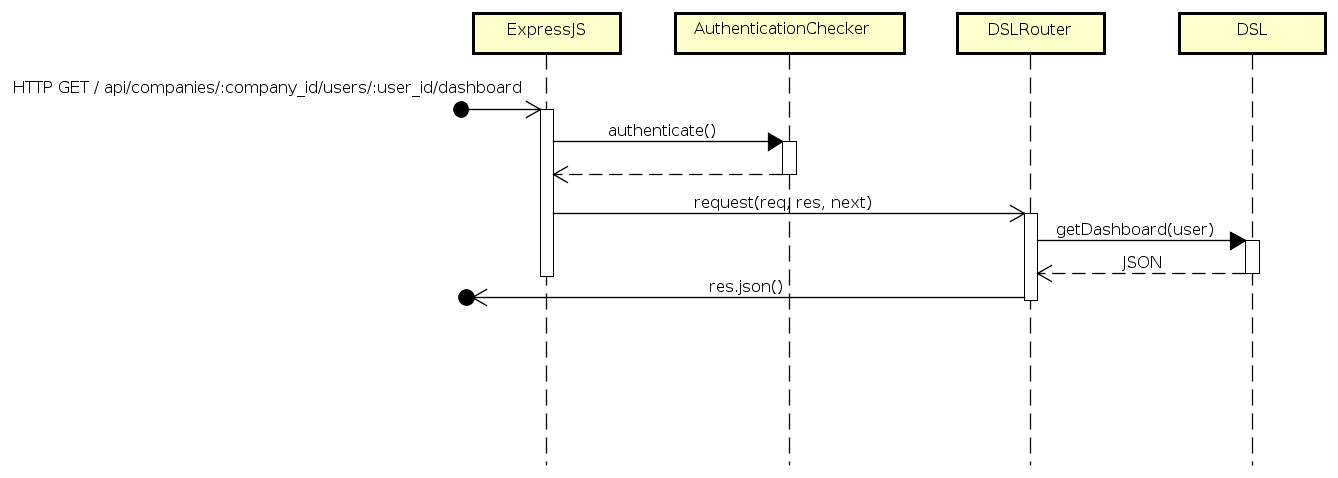
\includegraphics[width=0.8\textwidth]{res/sections/backend/sequence/(GET)dashboard.png}
\caption{Scenario dell'ottenimento della dashboard di un utente}
\end{figure}

\newpage
\paragraph{Esecuzione di una specifica DSL}\mbox{}\\
\textbf{Tipologia:} GET \\
\textbf{API:} /api/companies/:company\_id/DSLs/:dsl\_id/execute \\
\textbf{Livello di accesso minimo:} GUEST \\
\textbf{Descrizione:} Ritorna un JSON contenente i dati richiesti dalla specifica DSL e la struttura su cui inserire i dati. \\
\textbf{Scenario:} 
\begin{figure}[H]
\centering
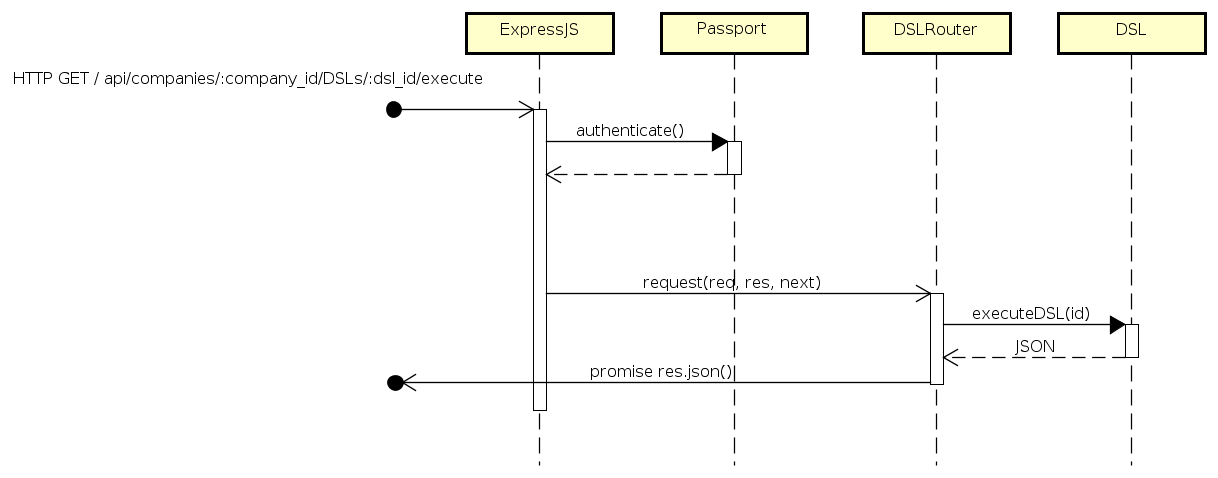
\includegraphics[width=0.8\textwidth]{res/sections/backend/sequence/(GET)dslByIDex.png}
\caption{Scenario dell'esecuzione di una specifica DSL}
\end{figure}

\newpage
\subsubsection{Database}
\paragraph{Elenco dei database della company}\mbox{}\\
\textbf{Tipologia:} GET \\
\textbf{API:} /api/companies/:company\_id/databases \\
\textbf{Livello di accesso minimo:} MEMBER \\
\textbf{Descrizione:} Ritorna un array contenente i nomi e gli id di ciascun database. \\
\textbf{Scenario:}
\begin{figure}[H]
\centering
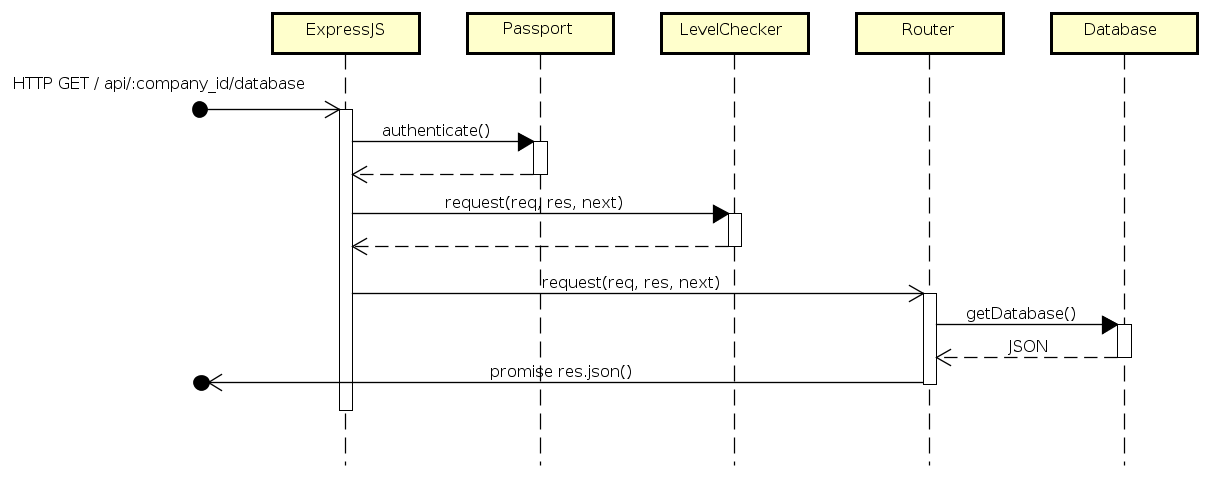
\includegraphics[width=0.8\textwidth]{res/sections/backend/sequence/(GET)database.png}
\caption{Scenario dell'elenco dei database propri della company}
\end{figure}

\newpage
\paragraph{Visualizzazione dati di un database}\mbox{}\\
\textbf{Tipologia:} GET \\
\textbf{API:} /api/companies/:company\_id/databases/:database\_id \\
\textbf{Livello di accesso minimo:} ADMIN \\
\textbf{Descrizione:} Ritorna tutte le informazioni relative al database richiesto. \\
\textbf{Scenario:} 
\begin{figure}[H]
\centering
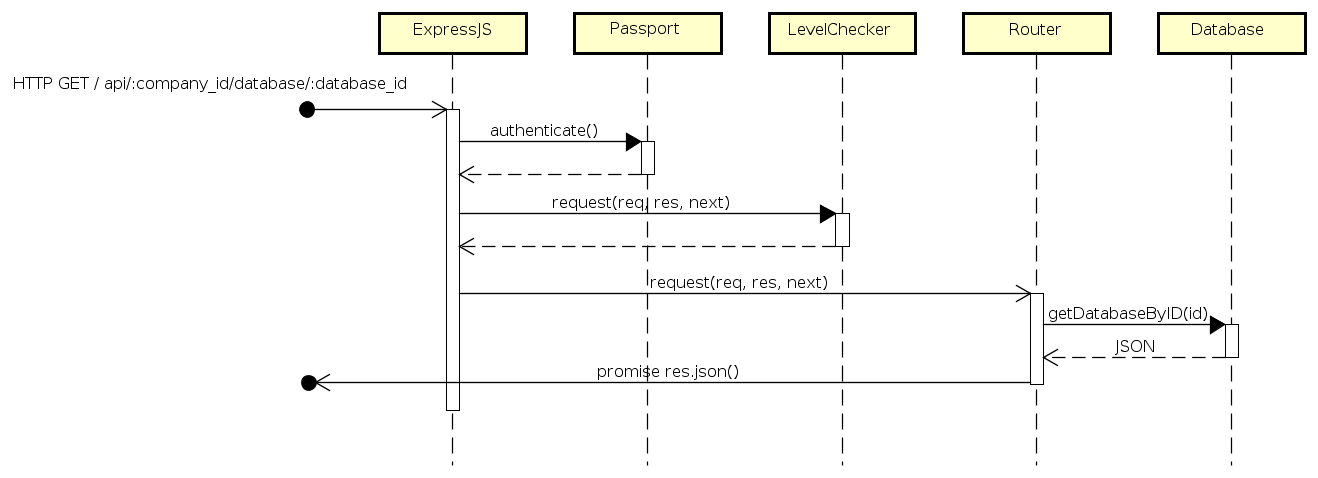
\includegraphics[width=0.8\textwidth]{res/sections/backend/sequence/(GET)databaseById.png}
\caption{Scenario della visualizzazione dei dati di un database}
\end{figure}

\newpage
\paragraph{Aggiunta di un database}\mbox{}\\
\textbf{Tipologia:} POST \\
\textbf{API:} /api/companies/:company\_id/databases \\
\textbf{Livello di accesso minimo:} ADMIN \\
\textbf{Descrizione:} Necessita di una richiesta con body contenete i dati relativi alla connessione del nuovo database. \\
\textbf{Scenario:}
\begin{figure}[H]
\centering
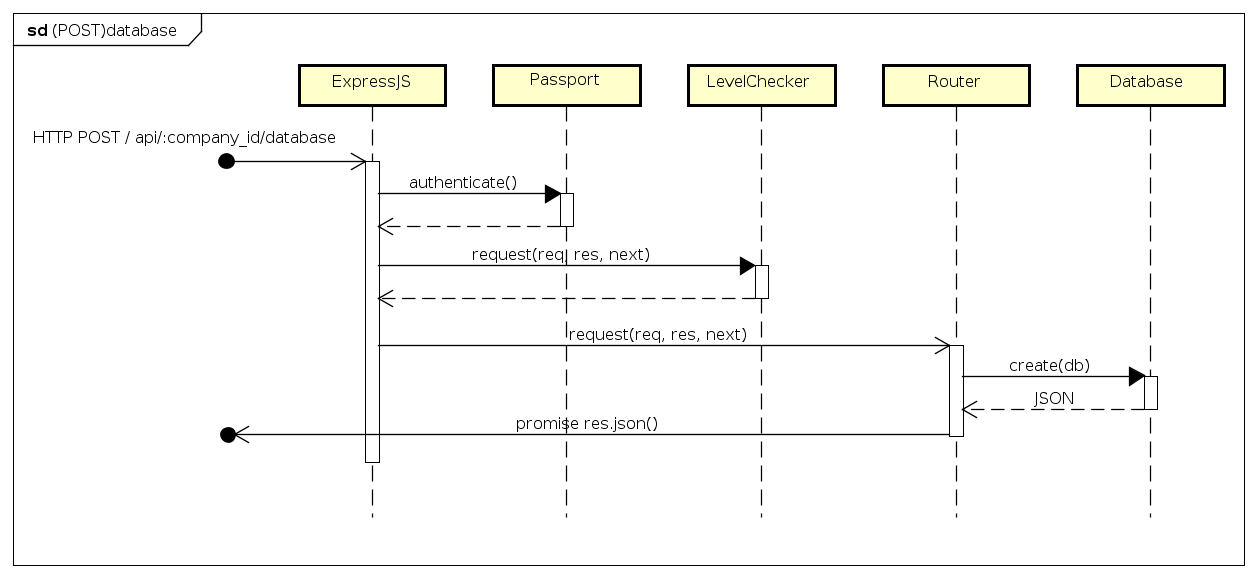
\includegraphics[width=0.8\textwidth]{res/sections/backend/sequence/(POST)database.png}
\caption{Scenario della creazione di una specifica DSL}
\end{figure}

\newpage
\paragraph{Aggiornamento di un database}\mbox{}\\
\textbf{Tipologia:} PUT \\
\textbf{API:} /api/companies/:company\_id/databases/:database\_id \\
\textbf{Livello di accesso minimo:} ADMIN \\
\textbf{Descrizione:} Metodo per aggiornare le informazioni relative alla connessione al database o per aggiornare l'elenco delle collezioni. \\
\textbf{Scenario:}
\begin{figure}[H]
\centering
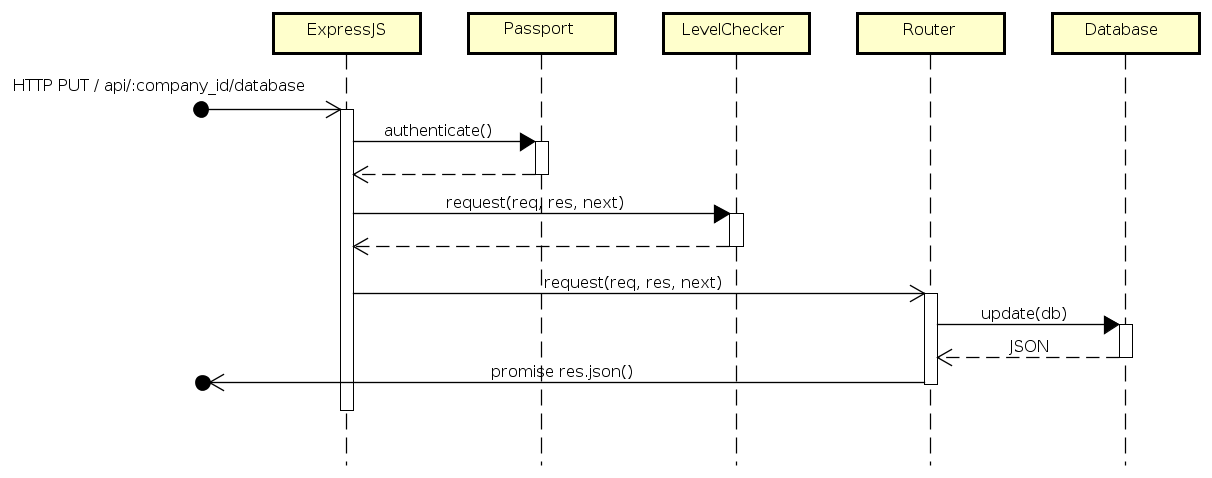
\includegraphics[width=0.8\textwidth]{res/sections/backend/sequence/(PUT)database.png}
\caption{Scenario dell'aggiornamento di un database}
\end{figure}

\newpage
\paragraph{Cancellazione di un database}\mbox{}\\
\textbf{Tipologia:} DELETE \\
\textbf{API:} /api/companies/:company\_id/databases/:database\_id \\
\textbf{Livello di accesso minimo:} ADMIN \\
\textbf{Descrizione:} Elimina il database selezionato e tutte le DSL che lo utilizzano. \\
\textbf{Scenario:} 
\begin{figure}[H]
\centering
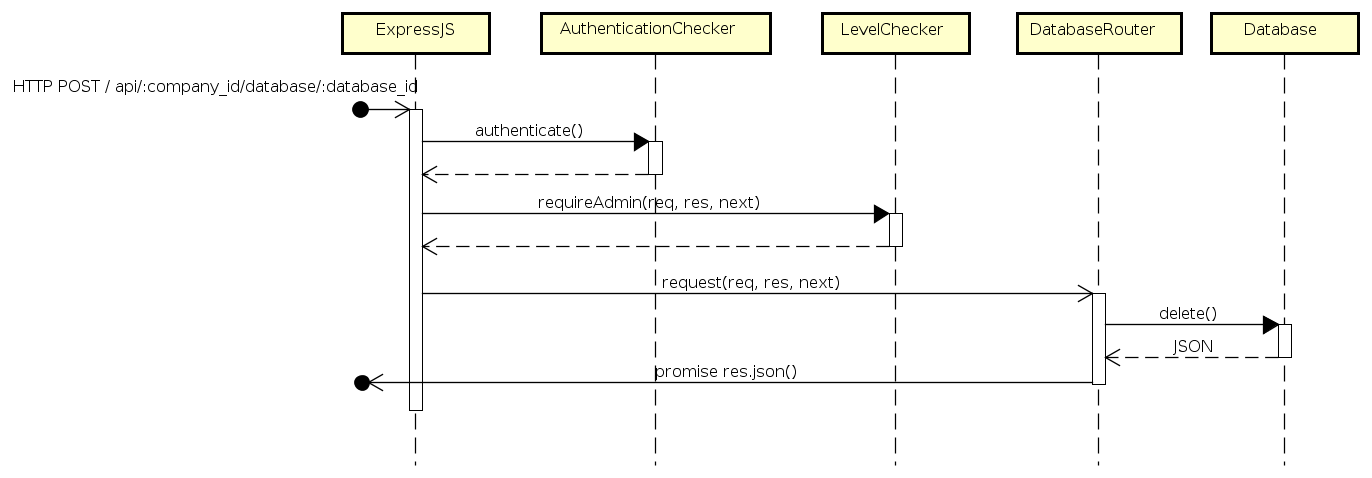
\includegraphics[width=0.8\textwidth]{res/sections/backend/sequence/(DELETE)database.png}
\caption{Scenario della cancellazione di un database}
\end{figure}

\newpage
\paragraph{Visualizzazione collections di un database} \mbox{}\\
\textbf{Tipologia:} GET \\
\textbf{API:} /api/companies/:company\_id/databases/:database\_id/collections \\
\textbf{Livello di accesso minimo:} MEMBER \\
\textbf{Descrizione:} Ritorna un array di collection relative ad un database a cui l'utente ha accesso. \\
\textbf{Scenario:} 
\begin{figure}[H]
\centering
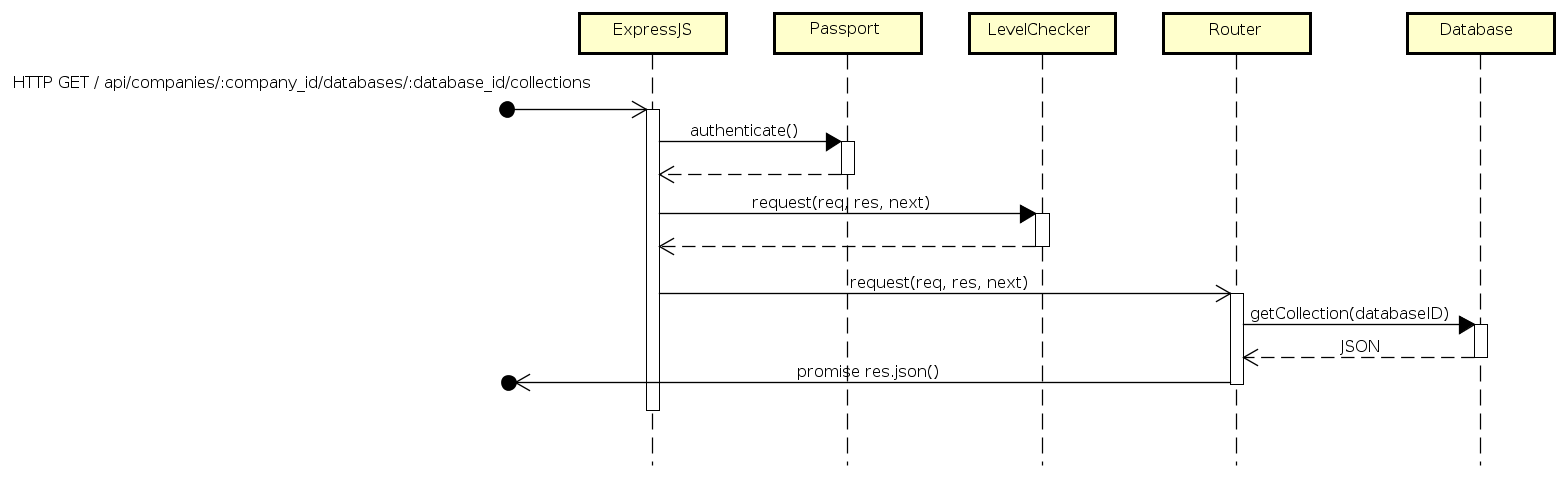
\includegraphics[width=0.8\textwidth]{res/sections/backend/sequence/(GET)collection.png}
\caption{Scenario della visualizzazione collections di un database}
\end{figure}

\newpage
\subsubsection{Super admin}
\paragraph{Ottenimento informazioni delle companies}\mbox{}\\
\textbf{Tipologia:} GET \\
\textbf{API:} /api/admin/companies \\
\textbf{Descrizione:} Restituisce un array di JSON contenenti le informazioni relative alle company presenti nell'applicazione. \\
\textbf{Scenario:} 
\begin{figure}[H]
\centering
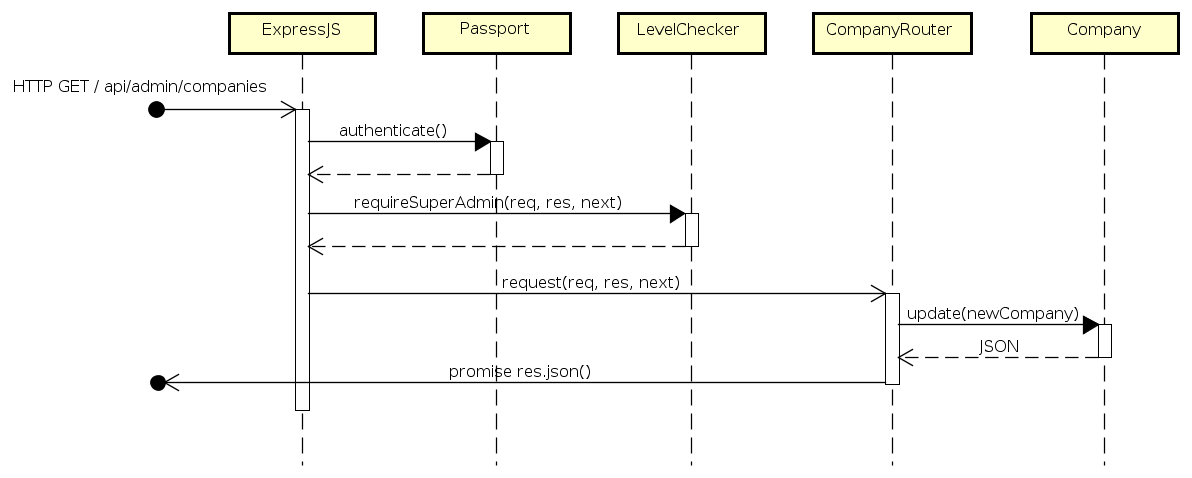
\includegraphics[width=0.8\textwidth]{res/sections/backend/sequence/(GET)companySA.png}
\caption{Scenario dell'ottenimento informazioni delle companies}
\end{figure}

\newpage
\paragraph{Aggiunta di un super admin}\mbox{}\\
\textbf{Tipologia:} POST \\
\textbf{API:} /api/admin/superadmins \\
\textbf{Descrizione:} Necessita di una richiesta con body contenente le informazioni relative al superadmin da creare. \\
\textbf{Scenario:} 
\begin{figure}[H]
\centering
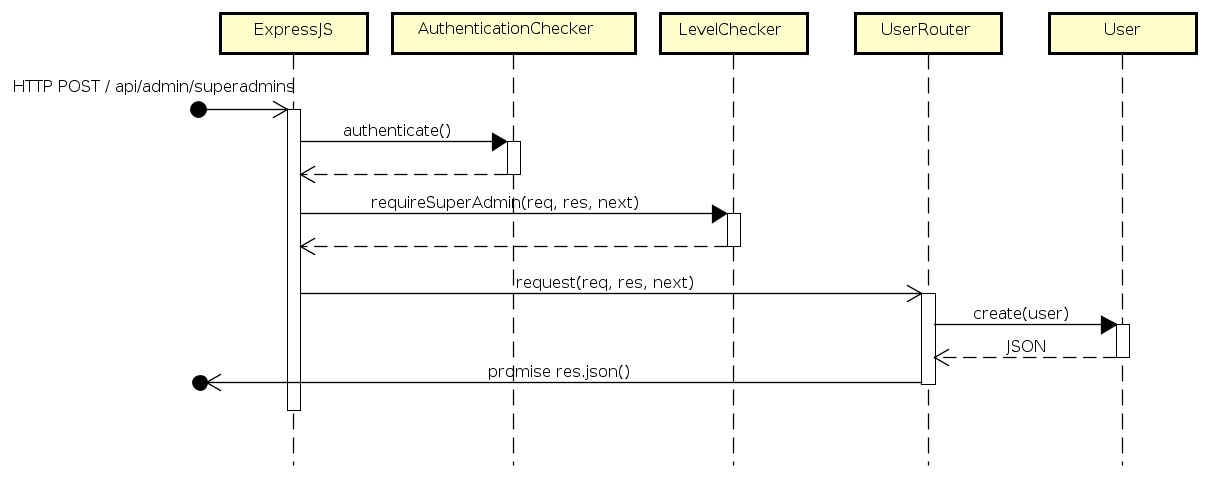
\includegraphics[width=0.8\textwidth]{res/sections/backend/sequence/(POST)superadmin.png}
\caption{Scenario dell'aggiunta di un super admin}
\end{figure}

\newpage
\paragraph{Aggiunta di un utente}\mbox{}\\
\textbf{Tipologia:} POST \\
\textbf{API:} /api/admin/companies/:company\_id/users \\
\textbf{Descrizione:} Necessita di una richiesta con body contenente le informazioni relative all'utente da creare per la company individuata da company\_id. \\
\textbf{Scenario:} 
\begin{figure}[H]
\centering
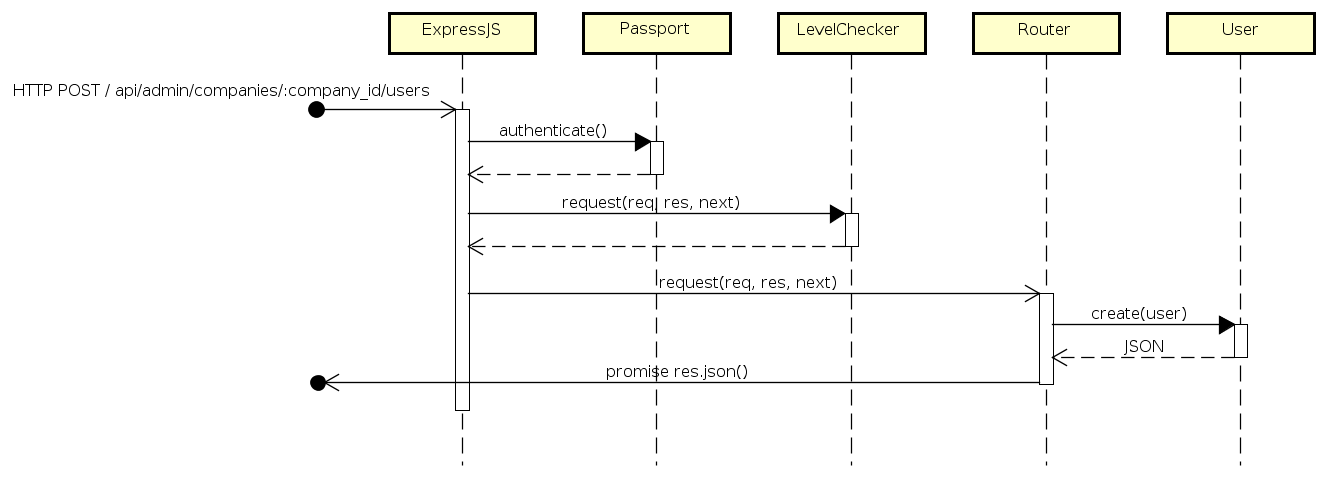
\includegraphics[width=0.8\textwidth]{res/sections/backend/sequence/(POST)userSA.png}
\caption{Scenario dell'aggiunta di un utente}
\end{figure}

\section{Frontend}

\subsection{Descrizione generale}

Il frontend dell'applicazione andrà a costituire il ruolo di \textit{View} nel pattern MVC. In particolare tale componente dell'applicazione è costituita da un sottosistema che implementa l'architettura \textit{Flux} proposta da \textit{Facebook}. Tale architettura si basa sul creare un sistema che abbia un \textit{data-flow} unidirezionale al fine di semplificare le interazioni tra le varie componenti e di assicurare che tra le componenti non esistano dipendenze circolari.
Nella progettazione secondo l'architettura \textit{Flux} si è seguito in particolare il principio che nessuna classe modifichi direttamente lo stato di un'altra ma che vengano create delle componenti che richiedono un'interazione delle \textit{Action} per comunicare con le altre parti del sistema.

\begin{figure}[h]
\centering
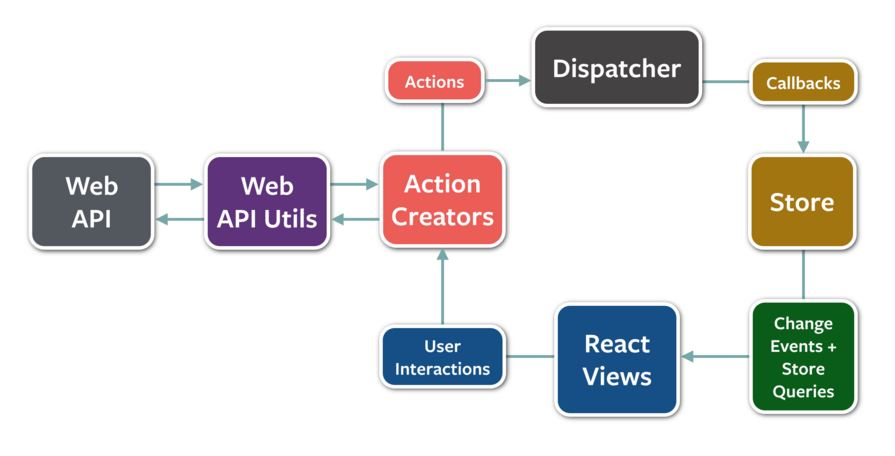
\includegraphics[width=0.8\textwidth]{res/sections/imgs/flux.jpg}
\caption{Diagramma dell'architettura Flux di Facebook}
\end{figure}
In un'architettura \textit{Flux} vengono distinti 4 componenti fondamentali:

\begin{itemize}
\item \textbf{Action}: Rappresenta un messaggio tra le componenti del sistema;
\item \textbf{Dispatcher}: funge da \textit{hub} centrale per le \textit{action} e si occupa di distribuirle al giusto \textit{store};
\item \textbf{Store}: contengono la logica applicativa del frontend e lo stato dei dati dall'ultimo \textit{update}. Si occupano di fornire i dati alle viste, quando queste li richiedono;
\item \textbf{View}: Sono la parte visiva dell'applicazione e, nel nostro caso, saranno costituite da componenti definite con React.
\end{itemize}

Dall'architettura sopra descritta sono stati individuati i seguenti package per il lato frontend di MaaS:

\begin{figure}[h]
\centering
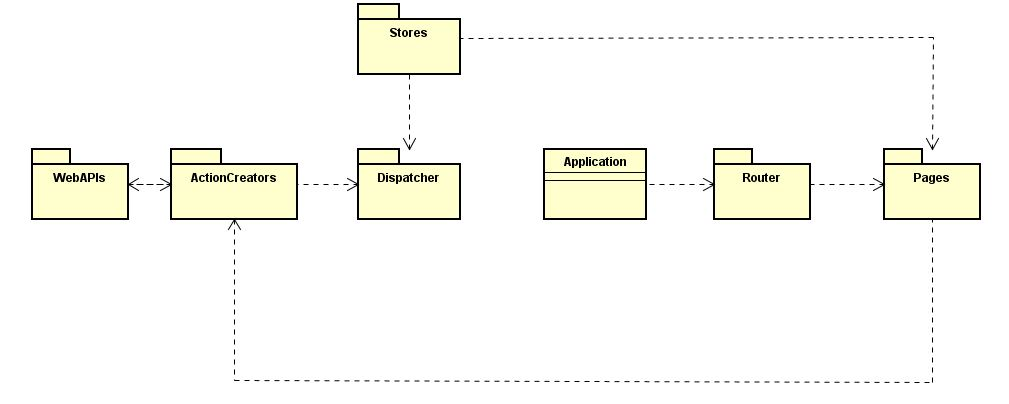
\includegraphics[width=0.8\textwidth]{res/sections/imgs/packages-diagram.jpg}
\caption{Diagramma dei package del frontend}
\end{figure}

\section{Descrizione dei package del frontend}
\subsection{WebAPIs}

\begin{figure}[h]
\centering
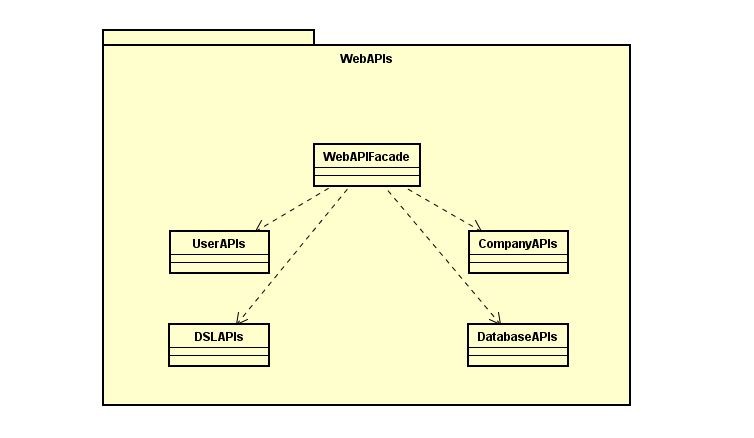
\includegraphics[width=0.8\textwidth]{res/sections/imgs/webapi-diagram.jpg}
\caption{Diagramma dei package del frontend}
\end{figure}

\paragraph*{Descrizione del package}
Il seguente package contiene tutte le classi che contengono i metodi per interagire con le API esposte dal server. 
\paragraph*{Classi contenute}
\begin{itemize}
\item \textbf{UserAPIs};
\item \textbf{CompanyAPIs};
\item \textbf{DSLAPIs};
\item \textbf{DatabaseAPIs};
\item \textbf{WebAPIFacade}.
\end{itemize}

\subsubsection{UserAPIs}
\paragraph*{Descrizione della classe}
Classe che espone tutti i metodi per interagire con le API del server che riguardano gli utenti.

\paragraph*{Utilizzo}
Viene utilizzata sia per il login sia per gestire le operazioni CRUD per le informazioni riguardanti gli utenti.

\paragraph*{Relazione con altre classi}
\begin{itemize}
\item ActionCreators::UserActionCreator
\end{itemize}

\subsubsection{CompanyAPIs}
\paragraph*{Descrizione della classe}
Classe che espone i metodi per interagire con le API esposte dal server che riguardano le Company.

\paragraph*{Utilizzo}
Contiene le operazioni CRUD per interagire con le informazioni riguardanti le company utilizzando le API esposte dal backend.

\paragraph*{Relazione con altre classi}
\begin{itemize}
\item ActionCreators::CompanyActionCreator
\end{itemize}

\subsubsection{DSLAPIs}
\paragraph*{Descrizione della classe}
Classe che espone i metodi per interagire con le API esposte dal server che riguardano le specifiche DSL.

\paragraph*{Utilizzo}
Viene utilizzata per lanciare le operazioni CRUD associate alle API esposte dal backend.

\paragraph*{Relazione con altre classi}
\begin{itemize}
\item ActionCreators::DSLActionCreator
\end{itemize}

\subsubsection{DatabaseAPIs}
\paragraph*{Descrizione della classe}
Classe per interagire con le API esposte dal server che riguardano i database delle Company.

\paragraph*{Utilizzo}
Viene utilizzata questa classe per lanciare le operazioni CRUD esposte dalle API del backend.

\paragraph*{Relazione con altre classi}
\begin{itemize}
\item ActionCreators::DatabaseAPIs
\end{itemize}

\subsubsection{WebAPIFacade}
\paragraph*{Descrizione della classe}
Classe che implementa il \textit{design pattern} \textit{Facade} al fine di creare un'interfaccia semplificata per il resto delle componenti per interagire con le API esposte dal backend.
\paragraph*{Utilizzo}
Questa classe viene utilizzata come interfaccia per il frontend per comunicare con le API esposte dal backend.
\paragraph*{Relazione con altre classi}
\begin{itemize}
\item webAPIs;
\item actionCreators.
\end{itemize} 

\subsection{ActionCreators}

\begin{figure}[h]
\centering
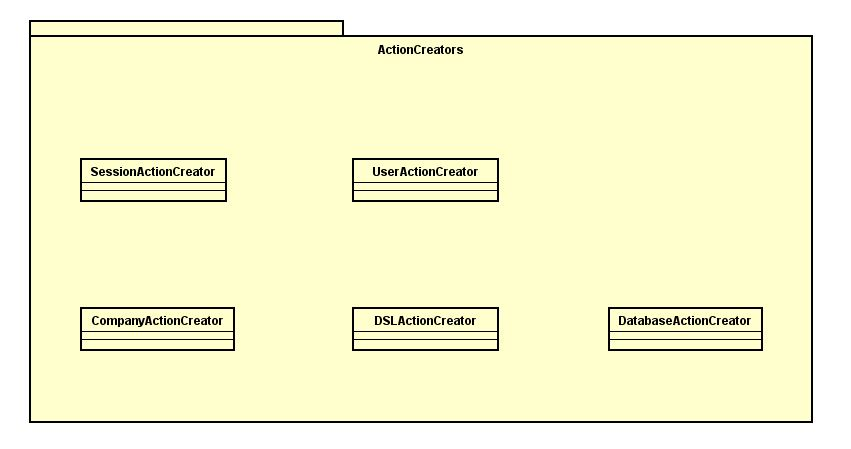
\includegraphics[width=0.8\textwidth]{res/sections/imgs/actioncreator-diagram.jpg}
\caption{Diagramma delle classi contenute in ActionCreators}
\end{figure}

\paragraph*{Descrizione del package}
Questo package contiene tutte le classi che si prestano come factory di Action. Le classi in questione mettono in relazione le webAPIs con il resto dell'applicazione, cioè vengono utilizzate per la richiesta delle funzionalità delle webAPIs per poi lanciare le Action relative alle risposte ricevute.

\paragraph*{Classi contenute}
\begin{itemize}
\item \textbf{SessionActionCreator};
\item \textbf{UserActionCreator};
\item \textbf{CompanyActionCreator};
\item \textbf{DSLActionCreator};
\item \textbf{DatabaseActionCreator}.
\end{itemize}

\subsubsection{SessionActionCreator}
\paragraph*{Descrizione della classe}
Classe che si occupa della gestione delle \textit{action} relative alla sessione corrente.

\paragraph*{Utilizzo}
Viene utilizzata per richiedere il login di un utente e per emanare le \textit{action} relative a login, sessione corrente e logout.

\paragraph*{Relazione con altre classi}
\begin{itemize}
\item Dispatcher;
\item Pages;
\item webAPIs::WebAPIFacade;
\item Stores::SessionStore.
\end{itemize}

\subsubsection{UserActionCreator}
\paragraph*{Descrizione della classe}
Classe che si occupa di creare e lanciare le \textit{action} relative agli utenti. Viene implementata tramite il \textit{design pattern} \textit{Factory}.
\paragraph*{Utilizzo}
Viene utilizzata per creare le \textit{action} relative agli utenti: la classe fornisce i metodi per utilizzare le \textit{webAPIs} contenute relative all'utente e restituisce le action che poi verrano reindirizzate a UserStore.

\paragraph*{Relazione con altre classi}
\begin{itemize}
\item Dispatcher;
\item Pages;
\item webAPIs::WebAPIFacade;
\item Stores::UserStore.
\end{itemize}

\subsubsection{CompanyActionCreator}
\paragraph*{Descrizione della classe}
Classe che si occupa dell'interazione dell'applicazione con CompanyAPIs e di lanciare \textit{Action} relative alle risposte ottenute da essa. Viene implementata tramite \textit{design pattern} \textit{Factory}.
\paragraph*{Utilizzo}
La classe viene utilizzata per creare le \textit{action} relative alle Company: sfrutta le \textit{webAPIs} dichiarate per interagire con il server e lancia le \textit{action} contenenti i dati ricevuti dalle API richieste.

\paragraph*{Relazione con altre classi}
\begin{itemize}
\item Dispatcher;
\item Pages;
\item Stores::CompanyStore;
\item webAPIs::WebAPIFacade.
\end{itemize}

\subsubsection{DSLActionCreator}
\paragraph*{Descrizione della classe}
Classe che si occupa di creare \textit{action} riguardanti le specifiche DSL.
\paragraph*{Utilizzo}
Tale classe viene utilizzata per sfruttare i metodi dichiarati dalle webAPIs per la richiesta delle API esposte dal server relative alle specifiche DSL. Dopo aver sfruttato l'API richiesta, la classe crea un'\textit{action} contenente i risultati ottenuti.

\paragraph*{Relazione con altre classi}
\begin{itemize}
\item Dispatcher;
\item Stores::DSLStore;
\item Pages;
\item webAPIs::WebAPIFacade.
\end{itemize}

\subsubsection{DatabaseActionCreator}
\paragraph*{Descrizione della classe}
Classe che si occupa di lanciare \textit{action} riguardanti le connessioni ai database di una Company.
\paragraph*{Utilizzo}
La classe viene utilizzata per richiamare i metodi definiti dalle \textit{webAPIs} relativi ai database delle Company e creare le action contenenti le risposte dai metodi chiamati.
\paragraph*{Relazione con altre classi}
\begin{itemize}
\item Dispatcher;
\item Pages;
\item Store::DatabaseStore;
\item webAPIs::WebAPIFacade.
\end{itemize}

\subsection{Dispatcher}
\paragraph*{Descrizione della classe}
Classe raffigurante il \textit{dispatcher} descritto nell'architettura Flux.
\paragraph*{Utilizzo}
Il dispatcher viene utilizzato come \textit{hub} centrale delle \textit{action} circolanti per l'applicazione. Esso deve fornire le informazioni per instradare le \textit{action} create dagli ActionCreators verso il giusto Store di destinazione
\paragraph*{Relazione con altre classi}
\begin{itemize}
\item Stores;
\item ActionCreators.
\end{itemize}


\subsection{Stores}

\begin{figure}[h]
\centering
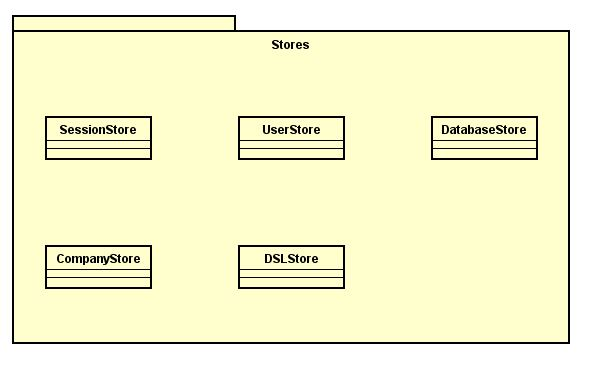
\includegraphics[width=0.8\textwidth]{res/sections/imgs/stores-diagram.jpg}
\caption{Diagramma delle classi per il package Stores}
\end{figure}

\paragraph*{Descrizione del package}
Il package in questione contiene le classi che implementano il concetto di Store presentato nell'architettura Flux. Ciascuno Store contiene dei dati omogenei tra loro e si occupa di fornirli alle pagine che ne necessitano.
\paragraph*{Classi contenute}
\begin{itemize}
\item \textbf{SessionStore};
\item \textbf{UserStore};
\item \textbf{DatabaseStore};
\item \textbf{CompanyStore};
\item \textbf{DSLStore}.
\end{itemize}

\subsubsection{SessionStore}
\paragraph*{Descrizione della classe}
Classe che contiene i dati relativi alla sessione corrente.
\paragraph*{Utilizzo}
Classe che viene utilizzata dall'applicazione per contenere e fornire i dati relativi alla sessione corrente. Si occupa di gestire le \textit{action} relative alla sessione e di conservarne i dati.
\paragraph*{Relazione con altre classi}
\begin{itemize}
\item Router;
\item Pages.
\end{itemize}

\subsubsection{UserStore}
\paragraph*{Descrizione della classe}
Classe che si occupa di contenere i dati relativi agli User.
\paragraph*{Utilizzo}
Questa classe viene utilizzata per mantenere i dati riguardanti gli utenti e di fornirli alle pagine che li richiedono.
\paragraph*{Relazione con altre classi}
\begin{itemize}
\item Pages;
\item Dispatcher.
\end{itemize}

\subsubsection{DatabaseStore}
\paragraph*{Descrizione della classe}
Classe che si occupa di contenere i dati relativi alle connessioni ai database definiti per le Company.
\paragraph*{Utilizzo}
Questa classe viene utilizzata per contenere i dati riguardanti le connessioni dei database definiti per le Company. Si occupa di ricevere dal dispatcher le \textit{action} relative a questi dati e di mantenere i dati riferiti.
\paragraph*{Relazione con altre classi}
\begin{itemize}
\item Pages;
\item Dispatcher.
\end{itemize}

\subsubsection{CompanyStore}
\paragraph*{Descrizione della classe}
Classe che si occupa di contenere i dati relativi alle Company.
\paragraph*{Utilizzo}
Questa classe viene utilizzata per ricevere le \textit{action} relative alle Company al fine di mantenere i dati relativi ad esse. Inoltre fornisce i metodi per fornire tali dati alle pagine che li richiedono
\paragraph*{Relazione con altre classi}
\begin{itemize}
\item Dispatcher;
\item Pages.
\end{itemize}

\subsubsection{DSLStore}
\paragraph*{Descrizione della classe}
Classe che si occupa di contenere i dati delle specifiche DSL
\paragraph*{Utilizzo}
Questa classe fornisce i metodi per ricevere le Action relative alle specifiche DSL e per mantenere i dati relativi ad esse. Fornisce inoltre i metodi per disporre quei dati per le pagine che li richiedono.
\paragraph*{Relazione con altre classi}
\begin{itemize}
\item Dispatcher;
\item Pages.
\end{itemize}


\subsection{Application}
\paragraph*{Descrizione della classe}
Questa è la classe principale del frontend: è la classe che richiama il Router e che inizializza il frontend.
\paragraph*{Utilizzo}
Viene utilizzata per inizializzare il frontend e per fornire le configurazioni necessarie al funzionamento per l'applicazione.

\subsection{Router}
\paragraph*{Descrizione della classe}
Questa classe è necessaria all'applicazione per determinare quale pagina mostrare.
\paragraph*{Utilizzo}
Viene istanziata nell'applicazione principale e determina le associazioni tra pagine e gli indirizzi URL per identificarle.

\subsection{Pages}
\paragraph*{Descrizione del package}
Questo package contiene tutte le pagine richiamate da Router. Ciascuna classe rappresenta una pagina definita come componente React e fornisce i metodi alla pagina per recuperare i dati da mostrare dagli store e i metodi per richiamare gli ActionCreators per la creazione di nuove Action.

\section{Editor}

Di seguito viengono elencati i casi d'uso per l'editor.

%\newpage da rimuovere?

\subsection{Casi d'Uso}


\subsubsection{UC-E}

    \begin{figure}[H]
      \begin{center}
        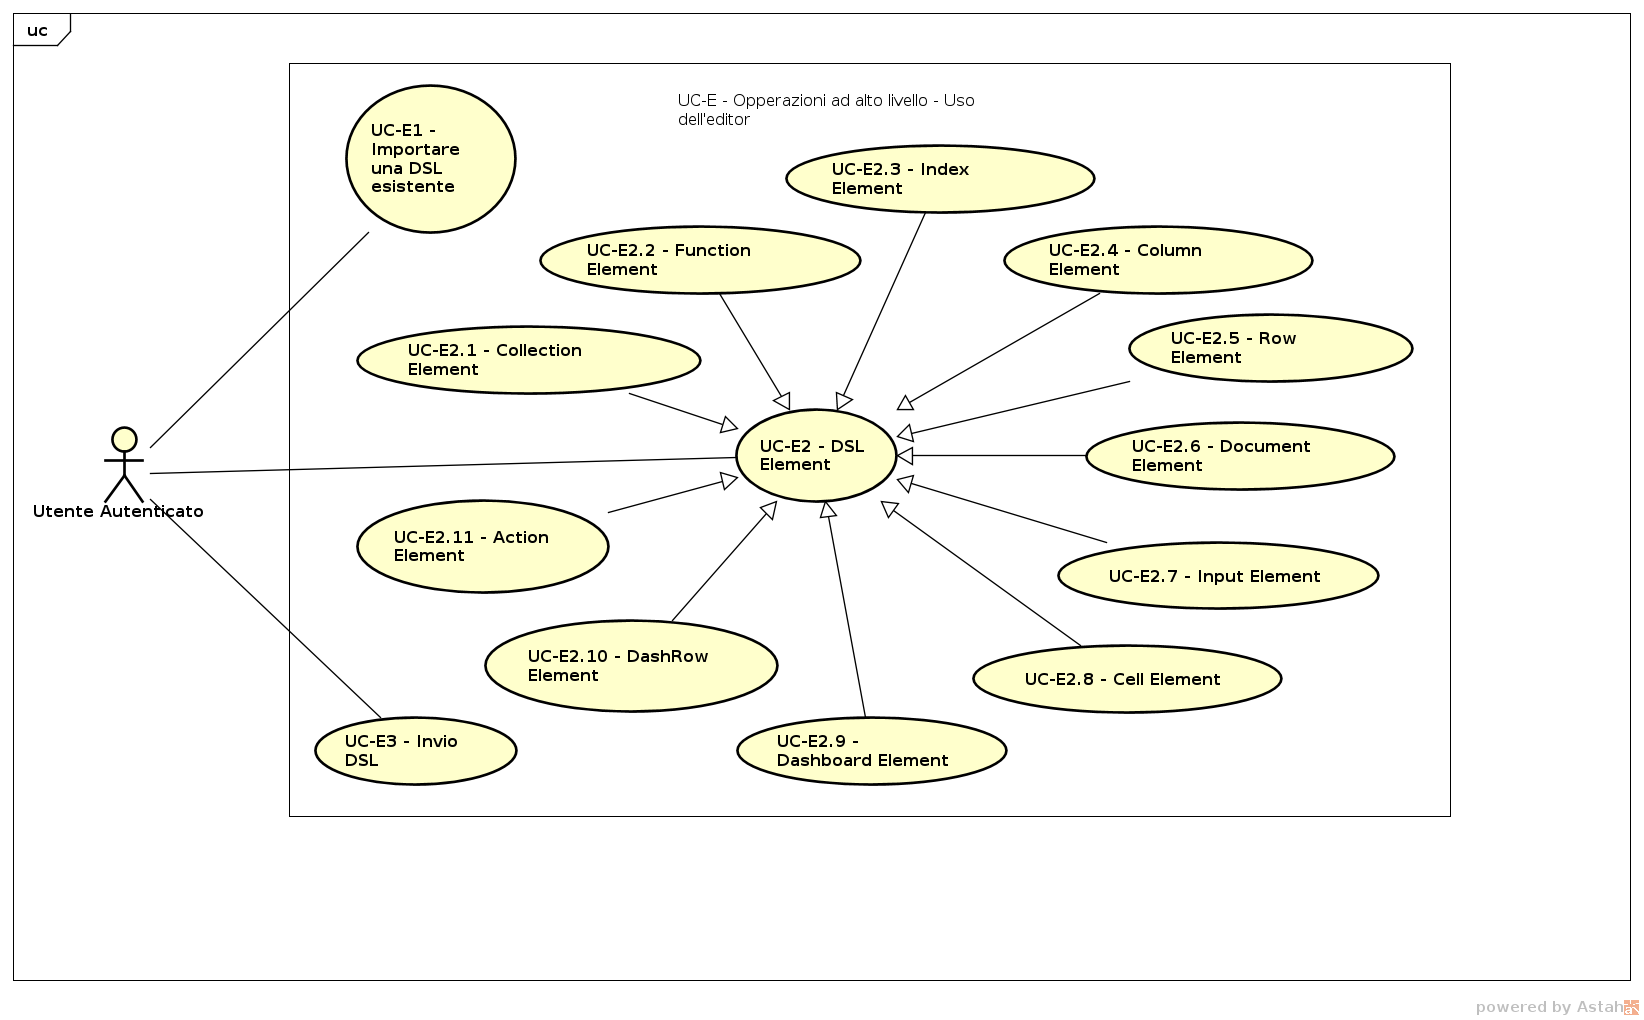
\includegraphics[width=12cm]{res/img/UCEditor/UC-E}
      \caption{UC-E - Operazioni ad alto livello - Uso dell'editor}
      \end{center} 
    \end{figure}    
    
    %Tabella 
    \begin{center}
      \bgroup
      \def\arraystretch{1.8}     
      \begin{longtable}{  p{3.5cm} | p{8cm} } 
        
        \hline
        \multicolumn{2}{ | c | }{ \cellcolor[gray]{0.9} \textbf{UC-E - Operazioni ad alto livello - Uso dell'editor}} \\ 
        \hline
        
        \textbf{Attori Primari} & Utente Autenticato, Ospite, Membro, Admin, Proprietario \\ 
        \textbf{Scopo e Descrizione} & 1. Importare un DSL esitente (UC-E1)
2. Manipolazione del DSL Element tramite l'interfaccia grafica dell'editor
3. Invio del DSL \\ 
        
        \textbf{Precondizioni}  & 1. Importare un DSL esitente (UC-E1)
2. Manipolazione del DSL Element tramite l'interfaccia grafica dell'editor
3. Invio del DSL \\ 
        
        \textbf{Postcondizioni} & L'utente ha utilizzato l'editor ed ha eseguito le azioni volute \\ 
        \textbf{Flusso Principale} & 1. Importare un DSL esistente
2. DSL element
3. Invio di un DSL \\
        \textbf{Estensioni} &  \\
        \textbf{Inclusioni} & 
      \end{longtable}
      \egroup
    \end{center} 


\subsubsection{UC-E2}

    \begin{figure}[H]
      \begin{center}
        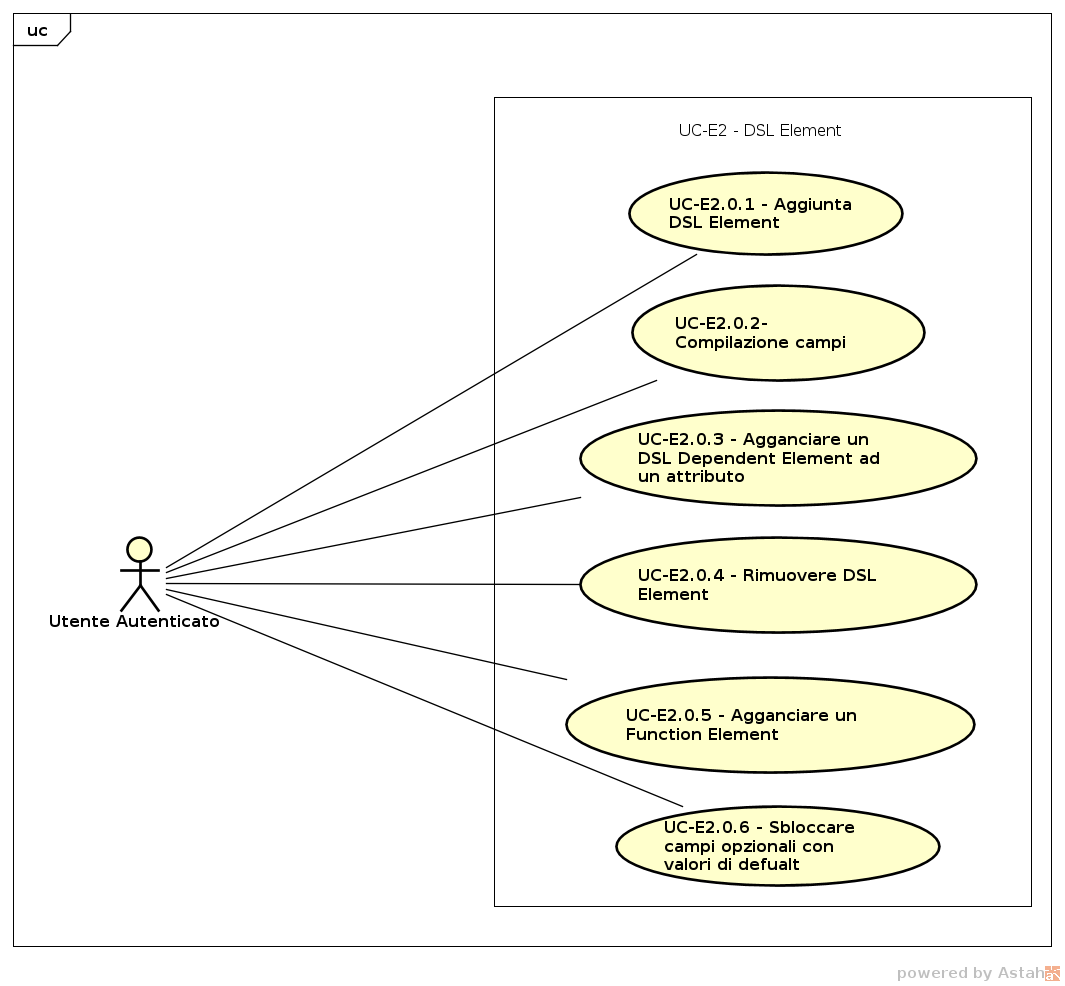
\includegraphics[width=12cm]{res/img/UCEditor/UC-E2-DSLElement}
      \caption{UC-E2 - DSL Element}
      \end{center} 
    \end{figure}    
    
    %Tabella 
    \begin{center}
      \bgroup
      \def\arraystretch{1.8}     
      \begin{longtable}{  p{3.5cm} | p{8cm} } 
        
        \hline
        \multicolumn{2}{ | c | }{ \cellcolor[gray]{0.9} \textbf{UC-E2 - DSL Element}} \\ 
        \hline
        
        \textbf{Attori Primari} & Utente Autenticato, Ospite, Membro, Admin, Proprietario \\ 
        \textbf{Scopo e Descrizione} & Il DSL element è la zona dove è possibile aggiungere, agganciare, sbloccare o rimuovere altri elementi del DSL. È possibile anche la compilazione dei campi. \\ 
        
        \textbf{Precondizioni}  & Il DSL element è la zona dove è possibile aggiungere, agganciare, sbloccare o rimuovere altri elementi del DSL. È possibile anche la compilazione dei campi. \\ 
        
        \textbf{Postcondizioni} & L'utente ha eseguito le sue operazioni sul DSL Element \\ 
        \textbf{Flusso Principale} & 1. Aggiunta DSL Element (UC-E2.0.1)
2. Compilazione campi (UC-E2.0.2)
3. Agganciare un DSL Dependent Element ad un attributo (UC-E2.0.3)
4. Rimuovere DSL Element (UC-E2.0.4)
5. Agganciare un Function Element (UC-E2.0.5)
6. Sbloccare campi opzionali con valori di default (UC-E2.0.6) \\
        \textbf{Estensioni} &  \\
        \textbf{Inclusioni} & 
      \end{longtable}
      \egroup
    \end{center} 


\subsubsection{UC-E2.0.1}

    %\begin{figure}[H]
    %  \begin{center}
    %    \includegraphics[width=12cm]{res/img/}
    %  \caption{UC-E2.0.1 - Aggiunta DSL Element}
    %  \end{center} 
    %\end{figure}    
    
    %Tabella 
    \begin{center}
      \bgroup
      \def\arraystretch{1.8}     
      \begin{longtable}{  p{3.5cm} | p{8cm} } 
        
        \hline
        \multicolumn{2}{ | c | }{ \cellcolor[gray]{0.9} \textbf{UC-E2.0.1 - Aggiunta DSL Element}} \\ 
        \hline
        
        \textbf{Attori Primari} & Utente Autenticato, Ospiete, Membro, Admin, Proprietario \\ 
        \textbf{Scopo e Descrizione} & L'utente ha la possibiltà di aggiungere un elemento DSL \\ 
        
        \textbf{Precondizioni}  & L'utente ha la possibiltà di aggiungere un elemento DSL \\ 
        
        \textbf{Postcondizioni} & L'utente ha aggiunto con successo un elemento DSL \\ 
        \textbf{Flusso Principale} &  \\
        \textbf{Estensioni} &  \\
        \textbf{Inclusioni} & 
      \end{longtable}
      \egroup
    \end{center} 
\subsubsection{UC-E2.0.2}

    %Tabella 
    \begin{center}
      \bgroup
      \def\arraystretch{1.8}     
      \begin{longtable}{  p{3.5cm} | p{8cm} } 
        
        \hline
        \multicolumn{2}{ | c | }{ \cellcolor[gray]{0.9} \textbf{UC-E2.0.2 - Compilazione campi}} \\ 
        \hline
        
        \textbf{Attori Primari} & Utente Autenticato, Ospite, Membro, Admin, Proprietario \\ 
        \textbf{Scopo e Descrizione} & L'utente ha la possibilit\`a di compilare i campi con del testo personalizzato \\ 
        
        \textbf{Precondizioni}  & L'utente ha la possibilit\`a di compilare i campi desiderati \\ 
        
        \textbf{Postcondizioni} & I campi desiderati dall'utente sono stati compilati con successo \\ 
        \textbf{Flusso Principale} &  \\
        \textbf{Estensioni} &  \\
        \textbf{Inclusioni} & 
      \end{longtable}
      \egroup
    \end{center}
\subsubsection{UC-E2.0.3}

    %Tabella 
    \begin{center}
      \bgroup
      \def\arraystretch{1.8}     
      \begin{longtable}{  p{3.5cm} | p{8cm} } 
        
        \hline
        \multicolumn{2}{ | c | }{ \cellcolor[gray]{0.9} \textbf{UC-E2.0.3 - Agganciare un DSL Dependent Element ad un attributo}} \\ 
        \hline
        
        \textbf{Attori Primari} & Utente Autenticato, Ospiete, Membro, Admin, Proprietario \\ 
        \textbf{Scopo e Descrizione} & Si da la possibilit\`a di agganciare un DSL Dependent Element ad un attributo. Questa azione \`e ripetibile diverse volte \\ 
        
        \textbf{Precondizioni}  & L'utente ha a disposizione un attributo e un DSL Dependent Element \\ 
        
        \textbf{Postcondizioni} & L'utente ha collegato con successo l'atributo e il DSL Dependent Element a disposizione \\ 
        \textbf{Flusso Principale} &  \\
        \textbf{Estensioni} &  \\
        \textbf{Inclusioni} & 
      \end{longtable}
      \egroup
    \end{center}
\subsubsection{UC-E2.0.4}

    %Tabella 
    \begin{center}
      \bgroup
      \def\arraystretch{1.8}     
      \begin{longtable}{  p{3.5cm} | p{8cm} } 
        
        \hline
        \multicolumn{2}{ | c | }{ \cellcolor[gray]{0.9} \textbf{UC-E2.0.4 - Rimuovere DSL Element}} \\ 
        \hline
        
        \textbf{Attori Primari} & Utente Autenticato, Ospite, Membro, Admin, Proprietario \\ 
        \textbf{Scopo e Descrizione} & \`E possibile rimuovere un DSL Element non pi\`u utilizzato o non pi\`u voluto \\ 
        
        \textbf{Precondizioni}  & L'utente sta visualizzando l'editor e il DSL Element che vuole eliminare esiste \\ 
        
        \textbf{Postcondizioni} & L'utente ha eliminato con successo il DSL Element \\ 
        \textbf{Flusso Principale} &  \\
        \textbf{Estensioni} &  \\
        \textbf{Inclusioni} & 
      \end{longtable}
      \egroup
    \end{center}
\subsubsection{UC-E2.0.5}

    %Tabella 
    \begin{center}
      \bgroup
      \def\arraystretch{1.8}     
      \begin{longtable}{  p{3.5cm} | p{8cm} } 
        
        \hline
        \multicolumn{2}{ | c | }{ \cellcolor[gray]{0.9} \textbf{UC-E2.0.5 - Agganciare un Function Element}} \\ 
        \hline
        
        \textbf{Attori Primari} & Utente Autenticato, Ospite, Membro, Admin, Proprietario \\ 
        \textbf{Scopo e Descrizione} & L'intento \`e quello di dare la possibilit\`a all'utilizzatore dell'editor di poter agganciare un Function Element a qualche suo attributo \\ 
        
        \textbf{Precondizioni}  & L'utente sta visualizzando l'editor e dispone di una Function Element collegabile \\ 
        
        \textbf{Postcondizioni} & L'utente ha agganciato con successo la Function Element \\ 
        \textbf{Flusso Principale} &  \\
        \textbf{Estensioni} &  \\
        \textbf{Inclusioni} & 
      \end{longtable}
      \egroup
    \end{center}
\subsubsection{UC-E2.0.6}

    %Tabella 
    \begin{center}
      \bgroup
      \def\arraystretch{1.8}     
      \begin{longtable}{  p{3.5cm} | p{8cm} } 
        
        \hline
        \multicolumn{2}{ | c | }{ \cellcolor[gray]{0.9} \textbf{UC-E2.0.6 - Sbloccare campi opzionali con valori di default}} \\ 
        \hline
        
        \textbf{Attori Primari} & Utente Autenticato, Ospite, Membro, Admin, Proprietario \\ 
        \textbf{Scopo e Descrizione} & Si da la possibilit\`a di sbloccare campi opzionali nel DSL assegnandogli valori di default \\ 
        
        \textbf{Precondizioni}  & L'utente ha la possibilit\`a di creare campi opzionali con valori di default \\ 
        
        \textbf{Postcondizioni} & L'utente ha creato campi opzionali con valori di default \\ 
        \textbf{Flusso Principale} &  \\
        \textbf{Estensioni} &  \\
        \textbf{Inclusioni} & 
      \end{longtable}
      \egroup
    \end{center}
\subsubsection{UC-E2.1}
 

    \begin{figure}[H]
      \begin{center}
        \includegraphics[width=12cm]{res/img/UCEditor/UC-2.1-CollectionElement}
      \caption{UC-E2.1 - Collection Element}
      \end{center} 
    \end{figure}

    %Tabella 
    \begin{center}
      \bgroup
      \def\arraystretch{1.8}     
      \begin{longtable}{  p{3.5cm} | p{8cm} } 
        
        \hline
        \multicolumn{2}{ | c | }{ \cellcolor[gray]{0.9} \textbf{UC-E2.1 - Collection Element}} \\ 
        \hline
        
        \textbf{Attori Primari} & Utente Autenticato, Ospite, Membro, Admin, Proprietario \\ 
        \textbf{Scopo e Descrizione} & Rappresentazione della sezione della parte della collection del DSL \\ 
        
        \textbf{Precondizioni}  & L'utente sta visualizzando l'editor \\ 
        
        \textbf{Postcondizioni} & L'utente ha gestito la gestione collection del DSL \\ 
        \textbf{Flusso Principale} & 1. Aggancia un Index Element (UC-E2.1.1)
2. Aggancia un Document Element (UC-E2.1.2) \\
        \textbf{Estensioni} &  \\
        \textbf{Inclusioni} & 
      \end{longtable}
      \egroup
    \end{center}
\subsubsection{UC-E2.1.1}

    %Tabella 
    \begin{center}
      \bgroup
      \def\arraystretch{1.8}     
      \begin{longtable}{  p{3.5cm} | p{8cm} } 
        
        \hline
        \multicolumn{2}{ | c | }{ \cellcolor[gray]{0.9} \textbf{UC-E2.1.1 - Aggancia un Index Element}} \\ 
        \hline
        
        \textbf{Attori Primari} & Utente Autenticato, Ospite, Membro, Admin, Proprietario \\ 
        \textbf{Scopo e Descrizione} & Unire alla collection creata un elemento Index del DSL \\ 
        
        \textbf{Precondizioni}  & La Collection esiste o \`e appena stata creata \\ 
        
        \textbf{Postcondizioni} & Un Index Element \`e stato agganciato a una Collection \\ 
        \textbf{Flusso Principale} &  \\
        \textbf{Estensioni} &  \\
        \textbf{Inclusioni} & 
      \end{longtable}
      \egroup
    \end{center}
\subsubsection{UC-E2.1.2}

    %Tabella 
    \begin{center}
      \bgroup
      \def\arraystretch{1.8}     
      \begin{longtable}{  p{3.5cm} | p{8cm} } 
        
        \hline
        \multicolumn{2}{ | c | }{ \cellcolor[gray]{0.9} \textbf{UC-E2.1.2 - Aggancia un Document Element}} \\ 
        \hline
        
        \textbf{Attori Primari} & Utente Autenticato, Ospite, Membro, Admin, Proprietario \\ 
        \textbf{Scopo e Descrizione} & Inserisce la sezione Show relativa alla collection creata nel DSL \\ 
        
        \textbf{Precondizioni}  & L'utente visualizza l'editor \\ 
        
        \textbf{Postcondizioni} & L'utente ha con successo agganciato una Show al Document Element \\ 
        \textbf{Flusso Principale} &  \\
        \textbf{Estensioni} &  \\
        \textbf{Inclusioni} & 
      \end{longtable}
      \egroup
    \end{center}
\subsubsection{UC-E2.2}
 

    \begin{figure}[H]
      \begin{center}
        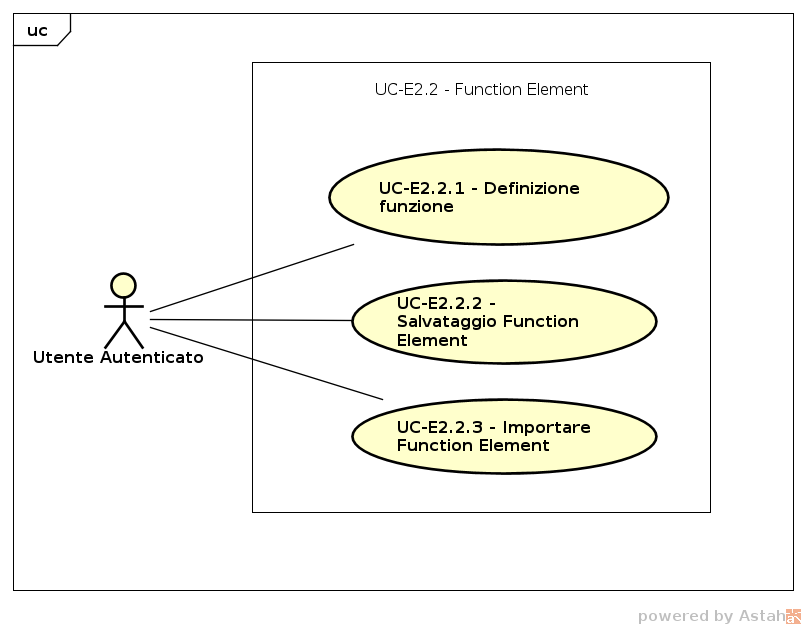
\includegraphics[width=12cm]{res/img/UCEditor/UC-E2.2-FunctionElement}
      \caption{UC-E2.2 - Function Element}
      \end{center} 
    \end{figure}

    %Tabella 
    \begin{center}
      \bgroup
      \def\arraystretch{1.8}     
      \begin{longtable}{  p{3.5cm} | p{8cm} } 
        
        \hline
        \multicolumn{2}{ | c | }{ \cellcolor[gray]{0.9} \textbf{UC-E2.2 - Function Element}} \\ 
        \hline
        
        \textbf{Attori Primari} & Utente Autenticato, Ospite, Membro, Admin, Proprietario \\ 
        \textbf{Scopo e Descrizione} & Rappresentare una canonica funzione in cui \`e possibile agganciare un elemento che verr\`a considerato un input e collegare l'output ad un altro DSL Element \\ 
        
        \textbf{Precondizioni}  & L'utente sta visualizzando l'editor \\ 
        
        \textbf{Postcondizioni} & L'utente ha collegato un function al valore del DSL desiderato \\ 
        \textbf{Flusso Principale} & 1. Definizione funzione (UC-E2.2.1)
2. Salvataggio Function Element (UC-E2.2.2)
3. Importare Function Element (UC-E2.2.3)  \\
        \textbf{Estensioni} &  \\
        \textbf{Inclusioni} & 
      \end{longtable}
      \egroup
    \end{center}
\subsubsection{UC-E2.2.1}

    %Tabella 
    \begin{center}
      \bgroup
      \def\arraystretch{1.8}     
      \begin{longtable}{  p{3.5cm} | p{8cm} } 
        
        \hline
        \multicolumn{2}{ | c | }{ \cellcolor[gray]{0.9} \textbf{UC-E2.2.1 - Definizione funzione}} \\ 
        \hline
        
        \textbf{Attori Primari} & Utente Autenticato, Ospite, Membro, Admin, Proprietario \\ 
        \textbf{Scopo e Descrizione} & L'utente ha la possibilit\`a di scrivere in un campo testo una funzione con il linguaggio definito da MaaS \\ 
        
        \textbf{Precondizioni}  & L'utente sta visualizzando l'editor \\ 
        
        \textbf{Postcondizioni} & L'utente ha definito con successo una funzione \\ 
        \textbf{Flusso Principale} &  \\
        \textbf{Estensioni} &  \\
        \textbf{Inclusioni} & 
      \end{longtable}
      \egroup
    \end{center}
\subsubsection{UC-E2.2.2}

    %Tabella 
    \begin{center}
      \bgroup
      \def\arraystretch{1.8}     
      \begin{longtable}{  p{3.5cm} | p{8cm} } 
        
        \hline
        \multicolumn{2}{ | c | }{ \cellcolor[gray]{0.9} \textbf{UC-E2.2.2 - Salvataggio Function Element}} \\ 
        \hline
        
        \textbf{Attori Primari} & Utente Autenticato, Ospite, Membro, Admin, Proprietario \\ 
        \textbf{Scopo e Descrizione} & L'utente ha la possibilit\`a di storicizzare la sua Function Element creata \\ 
        
        \textbf{Precondizioni}  & L'utente ha inserito una Function Element valida \\ 
        
        \textbf{Postcondizioni} & La Function Element \`e stata salvata con successo in MaaS \\ 
        \textbf{Flusso Principale} &  \\
        \textbf{Estensioni} &  \\
        \textbf{Inclusioni} & 
      \end{longtable}
      \egroup
    \end{center}
\subsubsection{UC-E2.2.3}

    %Tabella 
    \begin{center}
      \bgroup
      \def\arraystretch{1.8}     
      \begin{longtable}{  p{3.5cm} | p{8cm} } 
        
        \hline
        \multicolumn{2}{ | c | }{ \cellcolor[gray]{0.9} \textbf{UC-E2.2.3 - Importare Function Element}} \\ 
        \hline
        
        \textbf{Attori Primari} & Utente Autenticato, Ospite, Membro, Admin, Proprietario \\ 
        \textbf{Scopo e Descrizione} & Permette di importare nella sessione corrente una Function Element precedentemente definita \\ 
        
        \textbf{Precondizioni}  & L'utente ha i diritti per caricare la Function Element \\ 
        
        \textbf{Postcondizioni} & L'utente ha caricato la Function Element con successo \\ 
        \textbf{Flusso Principale} &  \\
        \textbf{Estensioni} &  \\
        \textbf{Inclusioni} & 
      \end{longtable}
      \egroup
    \end{center}
\subsubsection{UC-E2.3}
 

    \begin{figure}[H]
      \begin{center}
        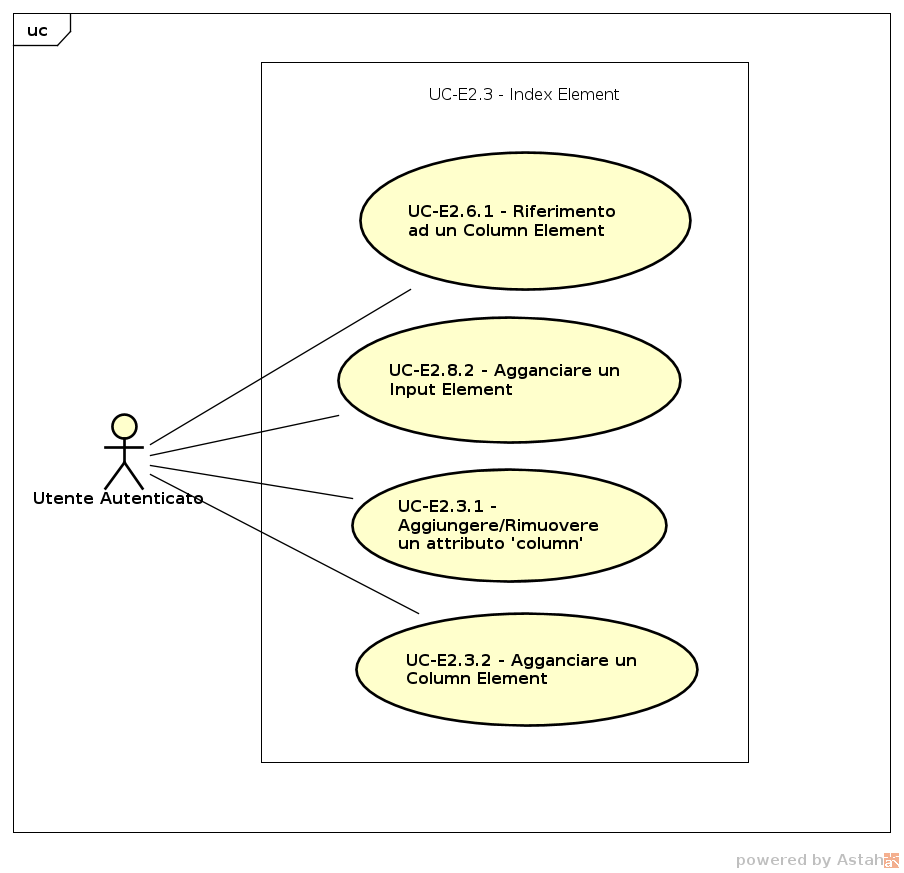
\includegraphics[width=12cm]{res/img/UCEditor/UC-E2.3-IndexElement}
      \caption{UC-E2.3 - Index Element}
      \end{center} 
    \end{figure}

    %Tabella 
    \begin{center}
      \bgroup
      \def\arraystretch{1.8}     
      \begin{longtable}{  p{3.5cm} | p{8cm} } 
        
        \hline
        \multicolumn{2}{ | c | }{ \cellcolor[gray]{0.9} \textbf{UC-E2.3 - Index Element}} \\ 
        \hline
        
        \textbf{Attori Primari} & Utente Autenticato, Ospite, Membro, Admin, Proprietario \\ 
        \textbf{Scopo e Descrizione} & Rappresentazione della sezione index del DSL nell'editor \\ 
        
        \textbf{Precondizioni}  & L'aggiunta dell'Index Element dev'essere eseguita in una Collection Element esistente \\ 
        
        \textbf{Postcondizioni} & \`E stata aggiunta la sezione Index alla Collection del DSL corrente \\ 
        \textbf{Flusso Principale} & 1. Riferimento ad un Column Element (UC-E2.6.1)
2. Agganciare un Input Element (UC-E2.8.2)
3. Aggiungere/Rimuovere un attributo ``column" (UC-E2.3.1)
4. Agganciare un Column Element (UC-E2.3.2) \\
        \textbf{Estensioni} &  \\
        \textbf{Inclusioni} & 
      \end{longtable}
      \egroup
    \end{center}
\subsubsection{UC-E2.3.1}

    %Tabella 
    \begin{center}
      \bgroup
      \def\arraystretch{1.8}     
      \begin{longtable}{  p{3.5cm} | p{8cm} } 
        
        \hline
        \multicolumn{2}{ | c | }{ \cellcolor[gray]{0.9} \textbf{UC-E2.3.1 - Aggiungere/Rimuovere un attributo ``column''}} \\ 
        \hline
        
        \textbf{Attori Primari} & Utente Autenticato, Ospite, Membro, Admin, Proprietario \\ 
        \textbf{Scopo e Descrizione} & Si da la possibilit\`a di rimuovere o aggiungere dall'Index un attributo \\ 
        
        \textbf{Precondizioni}  & Sia collegata a un Index Element \\ 
        
        \textbf{Postcondizioni} & Nel DSL nella sezione Index \`e aggiunto o rimosso un attributo ``column'' \\ 
        \textbf{Flusso Principale} &  \\
        \textbf{Estensioni} &  \\
        \textbf{Inclusioni} & 
      \end{longtable}
      \egroup
    \end{center}
\subsubsection{UC-E2.3.2}

    %Tabella 
    \begin{center}
      \bgroup
      \def\arraystretch{1.8}     
      \begin{longtable}{  p{3.5cm} | p{8cm} } 
        
        \hline
        \multicolumn{2}{ | c | }{ \cellcolor[gray]{0.9} \textbf{UC-E2.3.2 - Agganciare un Column Element}} \\ 
        \hline
        
        \textbf{Attori Primari} & Utente Autenticato, Ospite, Membro, Admin, Proprietario \\ 
        \textbf{Scopo e Descrizione} & \`E possibile agganciare un Column Element all'attributo ``column'' \\ 
        
        \textbf{Precondizioni}  & Deve essere presente un attributo Column \\ 
        
        \textbf{Postcondizioni} & La sezione del DSL ``column'' viene riempita con i valori impostati sul Column Element  \\ 
        \textbf{Flusso Principale} &  \\
        \textbf{Estensioni} &  \\
        \textbf{Inclusioni} & 
      \end{longtable}
      \egroup
    \end{center}
\subsubsection{UC-E2.4}

    %Tabella 
    \begin{center}
      \bgroup
      \def\arraystretch{1.8}     
      \begin{longtable}{  p{3.5cm} | p{8cm} } 
        
        \hline
        \multicolumn{2}{ | c | }{ \cellcolor[gray]{0.9} \textbf{UC-E2.4 - Column Element}} \\ 
        \hline
        
        \textbf{Attori Primari} & Utente Autenticato, Ospite, membro, Admin, Proprietario \\ 
        \textbf{Scopo e Descrizione} & Dare tutte le funzionalit\`a espresse nel DSL Element \\ 
        
        \textbf{Precondizioni}  & Deve riferirsi ad una struttura column presente nel DSL corrente \\ 
        
        \textbf{Postcondizioni} & L'utente manipola le parti che compongono la struttura \\ 
        \textbf{Flusso Principale} &  \\
        \textbf{Estensioni} &  \\
        \textbf{Inclusioni} & 
      \end{longtable}
      \egroup
    \end{center}
\subsubsection{UC-E2.5}

    %Tabella 
    \begin{center}
      \bgroup
      \def\arraystretch{1.8}     
      \begin{longtable}{  p{3.5cm} | p{8cm} } 
        
        \hline
        \multicolumn{2}{ | c | }{ \cellcolor[gray]{0.9} \textbf{UC-E2.5 - Row Element}} \\ 
        \hline
        
        \textbf{Attori Primari} & Utente Autenticato, Ospite, Membro, Admin, Proprietario \\ 
        \textbf{Scopo e Descrizione} & Rappresentazione di una struttura Row all'interno del DSL \\ 
        
        \textbf{Precondizioni}  & Dev'essere legata a una struttura Document \\ 
        
        \textbf{Postcondizioni} & Viene definita la struttura della Row all'interno del DSL corrente \\ 
        \textbf{Flusso Principale} &  \\
        \textbf{Estensioni} &  \\
        \textbf{Inclusioni} & 
      \end{longtable}
      \egroup
    \end{center}
\subsubsection{UC-E2.6}
 

    \begin{figure}[H]
      \begin{center}
        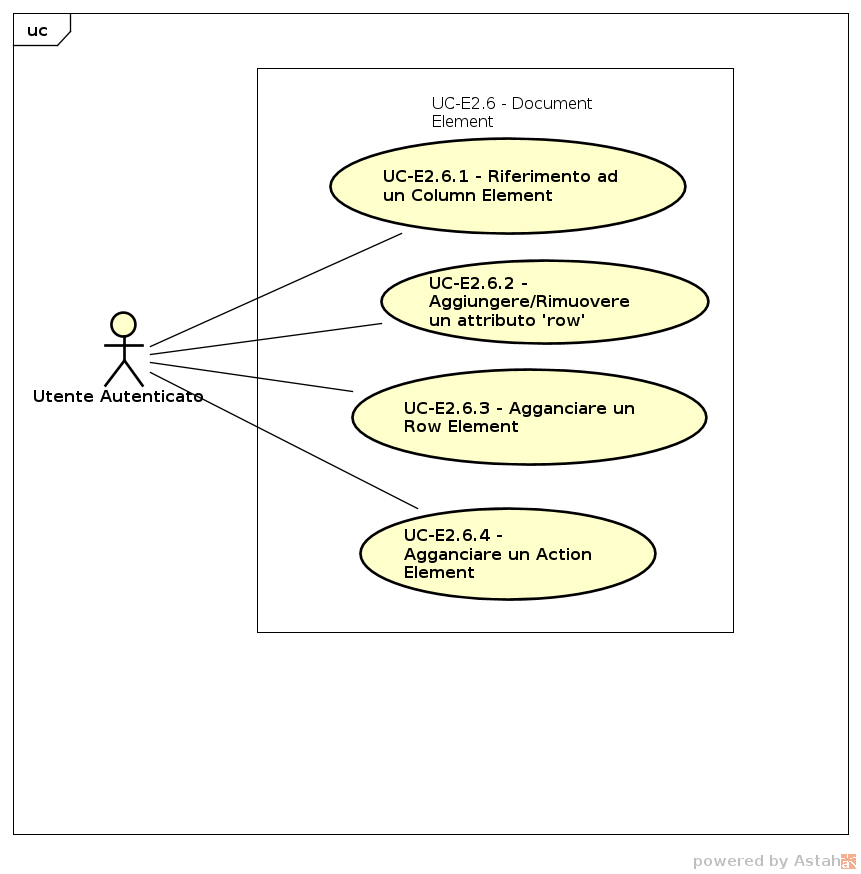
\includegraphics[width=12cm]{res/img/UCEditor/UC-E2.6-DocumentElement}
      \caption{UC-E2.6 - Document Element}
      \end{center} 
    \end{figure}

    %Tabella 
    \begin{center}
      \bgroup
      \def\arraystretch{1.8}     
      \begin{longtable}{  p{3.5cm} | p{8cm} } 
        
        \hline
        \multicolumn{2}{ | c | }{ \cellcolor[gray]{0.9} \textbf{UC-E2.6 - Document Element}} \\ 
        \hline
        
        \textbf{Attori Primari} & Utente Autenticato, Ospite, Membro, Admin, Proprietario \\ 
        \textbf{Scopo e Descrizione} & Rappresenta l'elemento Document del DSL \\ 
        
        \textbf{Precondizioni}  & L'utente visualizza l'editor \\ 
        
        \textbf{Postcondizioni} & Viene generato l'elemento Document nel DSL \\ 
        \textbf{Flusso Principale} & 1. Riferimento ad un Column Element (UC-E2.6.1)
2. Aggiungere/Rimuovere un attributo row (UC-E2.6.2)
3. Agganciare un Row Element (UC-E2.6.3)
4. Agganciare un Action Element (UC-E2.6.4) \\
        \textbf{Estensioni} &  \\
        \textbf{Inclusioni} & 
      \end{longtable}
      \egroup
    \end{center}
\subsubsection{UC-E2.6.1}

    %Tabella 
    \begin{center}
      \bgroup
      \def\arraystretch{1.8}     
      \begin{longtable}{  p{3.5cm} | p{8cm} } 
        
        \hline
        \multicolumn{2}{ | c | }{ \cellcolor[gray]{0.9} \textbf{UC-E2.6.1 - Riferimento ad un Column Element}} \\ 
        \hline
        
        \textbf{Attori Primari} & Utente Autenticato, Ospite, Membro, Admin, Proprietario \\ 
        \textbf{Scopo e Descrizione} & Riferirsi ad un elemento colonna precedentemente definito in modo da applicare la populate del DSL \\ 
        
        \textbf{Precondizioni}  & Esista almeno un elemento Document a cui si riferisca \\ 
        
        \textbf{Postcondizioni} & Viene composta la funzione populate \\ 
        \textbf{Flusso Principale} &  \\
        \textbf{Estensioni} &  \\
        \textbf{Inclusioni} & 
      \end{longtable}
      \egroup
    \end{center}
\subsubsection{UC-E2.6.2}

    %Tabella 
    \begin{center}
      \bgroup
      \def\arraystretch{1.8}     
      \begin{longtable}{  p{3.5cm} | p{8cm} } 
        
        \hline
        \multicolumn{2}{ | c | }{ \cellcolor[gray]{0.9} \textbf{UC-E2.6.2 - Aggiungere/Rimuovere un attributo row}} \\ 
        \hline
        
        \textbf{Attori Primari} & Utente Autenticato, Ospite, Membro, Admin, Proprietario \\ 
        \textbf{Scopo e Descrizione} & Aggiungere o rimuovere una struttura ``row'' all'interno del Document nella struttura DSL \\ 
        
        \textbf{Precondizioni}  & Si deve riferire a un Document esistente \\ 
        
        \textbf{Postcondizioni} & \`E stata manipolata (aggiunta o rimossa) una ``row'' all'interno del DSL Document \\ 
        \textbf{Flusso Principale} &  \\
        \textbf{Estensioni} &  \\
        \textbf{Inclusioni} & 
      \end{longtable}
      \egroup
    \end{center}
\subsubsection{UC-E2.6.3}

    %Tabella 
    \begin{center}
      \bgroup
      \def\arraystretch{1.8}     
      \begin{longtable}{  p{3.5cm} | p{8cm} } 
        
        \hline
        \multicolumn{2}{ | c | }{ \cellcolor[gray]{0.9} \textbf{UC-E2.6.3 - Agganciare un Row Element}} \\ 
        \hline
        
        \textbf{Attori Primari} & Utente Autenticato, Ospite, Membro, Admin, Proprietario \\ 
        \textbf{Scopo e Descrizione} & Definire la struttura della ``row'' del DSL  \\ 
        
        \textbf{Precondizioni}  & Sia presente un attributo ``row'' nel Document \\ 
        
        \textbf{Postcondizioni} & Nel DSL vengono trascritti nella struttura ``row'' gli attributi e i rispettivi valori \\ 
        \textbf{Flusso Principale} &  \\
        \textbf{Estensioni} &  \\
        \textbf{Inclusioni} & 
      \end{longtable}
      \egroup
    \end{center}
\subsubsection{UC-E2.6.4}

    %Tabella 
    \begin{center}
      \bgroup
      \def\arraystretch{1.8}     
      \begin{longtable}{  p{3.5cm} | p{8cm} } 
        
        \hline
        \multicolumn{2}{ | c | }{ \cellcolor[gray]{0.9} \textbf{UC-E2.6.4 - Agganciare un Action Element}} \\ 
        \hline
        
        \textbf{Attori Primari} & Utente Autenticato, Ospite, Membro, Admin, Proprietario \\ 
        \textbf{Scopo e Descrizione} & Legare il contenuto informativo della ``row'' all'azione definita dalla ``action'' \\ 
        
        \textbf{Precondizioni}  & \`E definita una ``row'' all'interno del DSL \\ 
        
        \textbf{Postcondizioni} & Verr\`a definita la ``action'' nella ``row'' \\ 
        \textbf{Flusso Principale} &  \\
        \textbf{Estensioni} &  \\
        \textbf{Inclusioni} & 
      \end{longtable}
      \egroup
    \end{center}
\subsubsection{UC-E2.7}
 

    \begin{figure}[H]
      \begin{center}
        \includegraphics[width=12cm]{res/img/UCEditor/UC-E2.7-InputElement}
      \caption{UC-E2.7 - Input Element}
      \end{center} 
    \end{figure}

    %Tabella 
    \begin{center}
      \bgroup
      \def\arraystretch{1.8}     
      \begin{longtable}{  p{3.5cm} | p{8cm} } 
        
        \hline
        \multicolumn{2}{ | c | }{ \cellcolor[gray]{0.9} \textbf{UC-E2.7 - Input Element}} \\ 
        \hline
        
        \textbf{Attori Primari} & Utente Autenticato, Ospite, Membro, Admin, Proprietario \\ 
        \textbf{Scopo e Descrizione} & Si occupa di rappresentare una dato in un specifico formato \\ 
        
        \textbf{Precondizioni}  & L'utente pu\`o visualizzare l'Editor \\ 
        
        \textbf{Postcondizioni} & Viene composto il dato con i valori inseriti dall'utente \\ 
        \textbf{Flusso Principale} & 1. Creare/Eliminare un nuovo attributo (UC-E2.7.1)
2. Modificare un attributo (UC-E2.7.2)
3. Comporre un attributo con sottoattributi (UC-E2.7.3) \\
        \textbf{Estensioni} &  \\
        \textbf{Inclusioni} & 
      \end{longtable}
      \egroup
    \end{center}
\subsubsection{UC-E2.7.1}

    %Tabella 
    \begin{center}
      \bgroup
      \def\arraystretch{1.8}     
      \begin{longtable}{  p{3.5cm} | p{8cm} } 
        
        \hline
        \multicolumn{2}{ | c | }{ \cellcolor[gray]{0.9} \textbf{UC-E2.7.1 - Creare/Eliminare un nuovo attributo}} \\ 
        \hline
        
        \textbf{Attori Primari} & Utente Autenticato, Ospite, Membro, Admin, Proprietario \\ 
        \textbf{Scopo e Descrizione} & Essendo il dato componibile da pi\`u attributi, permette di definire una coppia chiave/valore per meglio definire il suo dato \\ 
        
        \textbf{Precondizioni}  & L'utente si deve riferire a un Data Element presente \\ 
        
        \textbf{Postcondizioni} & Si manipola l'attributo selezionato \\ 
        \textbf{Flusso Principale} &  \\
        \textbf{Estensioni} &  \\
        \textbf{Inclusioni} & 
      \end{longtable}
      \egroup
    \end{center}
\subsubsection{UC-E2.7.2}

    %Tabella 
    \begin{center}
      \bgroup
      \def\arraystretch{1.8}     
      \begin{longtable}{  p{3.5cm} | p{8cm} } 
        
        \hline
        \multicolumn{2}{ | c | }{ \cellcolor[gray]{0.9} \textbf{UC-E2.7.2 - Modificare un attributo}} \\ 
        \hline
        
        \textbf{Attori Primari} & Utente Autenticato, Ospite, Membro, Admin, Proprietario \\ 
        \textbf{Scopo e Descrizione} & Poter rinominare o la chiave o il valore all'interno di un Data Element \\ 
        
        \textbf{Precondizioni}  & Ci sia un attributo a cui riferirsi \\ 
        
        \textbf{Postcondizioni} & Viene modificata o la chiave o il valore dell'attributo selezionato dall'utente \\ 
        \textbf{Flusso Principale} &  \\
        \textbf{Estensioni} &  \\
        \textbf{Inclusioni} & 
      \end{longtable}
      \egroup
    \end{center}
\subsubsection{UC-E2.7.3}

    %Tabella 
    \begin{center}
      \bgroup
      \def\arraystretch{1.8}     
      \begin{longtable}{  p{3.5cm} | p{8cm} } 
        
        \hline
        \multicolumn{2}{ | c | }{ \cellcolor[gray]{0.9} \textbf{UC-E2.7.3 - Comporre un attributo con sottoattributi}} \\ 
        \hline
        
        \textbf{Attori Primari} & Utente Autenticato, Ospite, Membro, Admin, Proprietario \\ 
        \textbf{Scopo e Descrizione} & Un utente \`e in grado di poter definire strutture complesse per i suoi scopi \\ 
        
        \textbf{Precondizioni}  & Ci sia un Data Element a cui riferirsi \\ 
        
        \textbf{Postcondizioni} & L'attributo del dato \`e a sua volta costituito da altri attributi \\ 
        \textbf{Flusso Principale} &  \\
        \textbf{Estensioni} &  \\
        \textbf{Inclusioni} & 
      \end{longtable}
      \egroup
    \end{center}

\section{Interprete}
\subsection{Diagrammi della classi}
L'interprete è la componente di MaaS che si occupa della conversione da DSL Structure in DSL. Questa decisione è stata presa per poter avere una rappresentazione semplice da manipolare attraverso l'editor e facile da ricondurre nel formato testuale.

La progettazione ha seguito un approccio bottom-up, con la creazione delle componenti per il funzionamento, incluse in un package e inserito un Facade per semplificarne l'uso. I patter usati sono Facade, Singleton e Chain of Responsability.
\subsection{Package DSLInterpreter}
\begin{figure}[H]
  \centering
  \includegraphics[width=0.9\textwidth]{res/img/Diagram_Interpreter.png}
  \caption{Package DSLInterpreter}
  \label{fig:diagram_model}
\end{figure}
\subsubsection{Descrizione}
In questo package vengono inserite tutte le classi che contribuiscono alla traduzione dal DSL Structure prodotto dall'editor all'equivalente DSL.
La classe DSLInterpreter implementa il Chain of Responsability dove detiene una lista di tutti gli interpreti da invocare man mano che vengono applicate le traduzioni. Il risultato di ogni interprete verrà contatenato e come risultato si otterrà il DSL richiesto.
Il FacadeEditorInterpreter implementa il patter Facade per offrire un interfaccia semplice per attuare la traduzione rendendo nascoste i componenti per applicarla.
\subsubsection{DSLInterpreter::FacadeInterpreter}
\begin{itemize}
\item \textbf{Descrizione} \hfill \\
  Rappresenta l'implementazione del pattern Facade.
\item \textbf{Utilizzo} \hfill \\
  Permette di interfacciarsi al modulo richiedendo eslusivamente la traduzione da DSL Structure a DSL. Questo oltre a semplificare al client la gestione della traduzione, nasconde l'implementazione rendendo il modulo maggiormente mantenibile.
\item \textbf{Relazioni con altre classi} \hfill
  \begin{itemize}
  \item DSLInterpreter::StoreDSL
  \item DSLInterpreter::IDSLInterpreter
  \end{itemize}
\end{itemize}
\subsubsection{DSLInterpreter::StoreDSL}
\begin{itemize}
\item \textbf{Descrizione} \hfill \\
  Mantiene il riferimento dal DSL Structure da tradurre.
\item \textbf{Utilizzo} \hfill \\
  Viene usata dalle implementazioni di \texttt{DSLInterpreter::DSLInterpreter} per ottenere l'oggetto riferito da un attributo della struttura da tradurre. Questi casi si riscontrano nella definizione di un componente del DSL in cui sono innestati altri componenti ( es. DSL Collection con DSL Index e DSL Document ).

  Ciò permette di non violare il Single Responsability Principle, in quanto i vari interpreti conoscono solo la struttura del singolo componente da interpretare e non detengono un possibile accesso dell'intera DSL Structure.
\item \textbf{Relazione con altre classi} \hfill
  \begin{itemize}
  \item DSLInterpreter::DSLFacadeInterpreter
  \item DSLInterpreter::DSLInterpreter
  \end{itemize}
\end{itemize}
\subsubsection{DSLInterpreter::DSLInterpreter}
\begin{itemize}
\item \textbf{Descrizione}
  Implementa il Chain of Responsabiltity mantenendo una lista di tutti gli interpreti da avviare e fornisce i metodo da implementare per i vari interpreti.
\item \textbf{Utilizzo}
  Mantiene struttura dati ed il comportamento comune degli interpreti. In più attraverso il metodo interpret viene definita la sequenza per portare a compito la traduzione di una componente del DSL.
\item \textbf{Relazione con altre classi} \hfill
  \begin{itemize}
  \item DSLInterpreter::FacadeInterpreter
  \item DSLInterpreter::StoreDSL
  \item DSLInterpreter::ActionInterpreter
  \item DSLInterpreter::CellInterpreter
  \item DSLInterpreter::RowInterpreter
  \item DSLInterpreter::ColumnInterpreter
  \item DSLInterpreter::DashboardInterpreter
  \item DSLInterpreter::CollectionInterpreter
  \item DSLInterpreter::DashRowInterpreter
  \item DSLInterpreter::DocumentInterpreter
  \item DSLInterpreter::FunctionInterpreter
  \item DSLInterpreter::IndexInterpreter
  \item DSLInterpreter::InputInterpreter
  \end{itemize}
\end{itemize}


\section{Diagrammi di attività}
In seguito vengono descritte le interazioni dell'utente con MaaS utilizzando i diagrammi di attività, secondo la seguente struttura:
\begin{itemize}
\item \textbf{Utente non autenticato};
\item \textbf{Utente autenticato};
\item \textbf{Super admin}.
\end{itemize}
\subsection{Utente non autenticato}
\begin{figure}[H]
\begin{center}
\includegraphics[height=12cm]{res/sections/backend/activities/principaliSenzaAuth.png}
\caption{Attività principali per un utente non autenticato}
\end{center}
\end{figure}
Un utente non autenticato, una volta visualizzata la pagina di MaaS, può:
\begin{itemize}
\item registrarsi, a seguito di un invito di un owner di una company;
\item effettuare il login;
\item eseguire la procedura di recupero password;
\item creare una nuova Company. L'utente verrà registrato come owner della company appena creata.
\end{itemize}
\subsubsection{Registrazione}
\begin{figure}[H]
\begin{center}
\includegraphics[height=12cm]{res/sections/backend/activities/registrazione.png}
\caption{Registrazione a MaaS}
\end{center}
\end{figure}
L'utente si trova nella pagina di registrazione a MaaS. Indirizzo email e password sono già stati impostati, e potrenno essere modificati dopo il completamento della procedura di registrazione; viene richiesto l'inserimento di tre campi base per il profilo di un utente: nome, cognome e data di nascita.
\subsubsection{Login}
\begin{figure}[H]
\begin{center}
\includegraphics[height=12cm]{res/sections/backend/activities/registrazione.png}
\caption{Login}
\end{center}
\end{figure}
L'utente non autenticato deve inserire, in due caselle di testo, le proprie credenziali di accesso, username e password, per poter accedere a MaaS. Se le credenziali risultano valide l'utente veràà reindirizzato alla pagina contenente la propria dashboard, altrimenti verrà mostrato un messaggio di errore.
\subsubsection{Recupero password}
\begin{figure}[H]
\begin{center}
\includegraphics[height=12cm]{res/sections/backend/activities/recuperoPassword.png}
\caption{Recupero password}
\end{center}
\end{figure}
L'utente non autenticato deve inserire, in una casella di testo, l'indirizzo email al quale sarà inviato il codice segreto da utilizzare nella procedura di reset della password.
\subsubsection{Reset password}
\begin{figure}[H]
\begin{center}
\includegraphics[height=12cm]{res/sections/backend/activities/resetPassword.png}
\caption{Reset password}
\end{center}
\end{figure}
L'utente non autenticato deve inserire, in una casella di testo, il codice segreto che ha ricevuto tramite email necessario a eseguire il reset della password. Se il codice è verificato, l'utente non autenticato potrà inserire una nuova password, che verrà memorizzata al posto della vecchia.
\subsubsection{Creazione company}
\begin{figure}[H]
\begin{center}
\includegraphics[height=12cm]{res/sections/backend/activities/creazioneCompany.png}
\caption{Creazione company}
\end{center}
\end{figure}
L'utente non autenticato che crea una company viene registrato come suo owner. È pertanto necessario fornire, durante la procedura di creazione, l'indirizzo email e la password dell'utente, oltre che il nome della company stessa.
\newpage
\subsection{Utente autenticato}
\begin{figure}[H]
\begin{center}
\includegraphics[width=18cm,angle=90]{res/sections/backend/activities/principaliConAuth.png}
\caption{Attività principali per un utente autenticato}
\end{center}
\end{figure}
Dopo aver effettuato il login un utente può:
\begin{itemize}
\item visualizzare le proprie credenziali di accesso, modificarle o rimuoversi da MaaS;
\item eseguire operazioni che coinvolgono specifiche DSL;
\item eseguire operazioni sulla sua dashboard;
\item gestire i permessi degli altri utenti (solo per admin e owner);
\item gestire gli utenti della company(solo per admin e owner);
\item visualizzare e gestire (quest'ultima solo per admin e owner) i database della company;
\item effettuare il logout.
\end{itemize}
\subsubsection{Modifica delle credenziali utente}
\begin{figure}[H]
\begin{center}
\includegraphics[height=12cm]{res/sections/backend/activities/modificaCredenziali.png}
\caption{Modifica delle credenziali utente}
\end{center}
\end{figure}
L'utente autenticato, dopo aver visualizzato la pagina con i suoi dati personali, può decidere di modificare le proprie credenziali di accesso inseremdo email e passowrd. Nel caso in cui le credenziali non siano valide (ad esempio, in caso di inserimento di un indirizzo email già presente) verrà visualizzato un messaggio di errore nel momento di invio della richiesta di modifica.
\subsubsection{Rimozione dell'utente}
\begin{figure}[H]
\begin{center}
\includegraphics[height=12cm]{res/sections/backend/activities/rimuoviProfilo.png}
\caption{Rimozione dell'utente}
\end{center}
\end{figure}
L'utente autenticato, dopo aver visualizzato la pagina con i suoi dati personali, può decidere di cancellarsi da MaaS. Viene proposta una richiesta di conferma per evitare eliminazioni accidentali. Se la richiesta viene confermata, l'utente è rimosso da MaaS.
\subsubsection{Operazioni su specifiche DSL}
\begin{figure}[H]
\begin{center}
\includegraphics[height=12cm]{res/sections/backend/activities/operazioniDSL.png}
\caption{Operazioni su specifiche DSL}
\end{center}
\end{figure}
Un utente autenticato può decidere di effettuare varie operazioni sulle specifiche DSL alle quali ha accesso; in particolare:
\begin{itemize}
\item eseguire una specifica DSL, e visualizzare il risultato in forma tabellare;
\item modificare una specifica DSL;
\item creare una specifica DSL;
\item leggere il codice della specifica DSL.
\end{itemize}
Le ultime tre operazioni coinvolgono l'editor fornito da MaaS.
\subsubsection{Operazioni sulla dashboard}
\begin{figure}[H]
\begin{center}
\includegraphics[height=12cm]{res/sections/backend/activities/operazioniDashboard.png}
\caption{Operazioni sulla dashboard}
\end{center}
\end{figure}
Un utente autenticato può decidere di effettuare varie operazioni sulla propria dashboard; in particolare:
\begin{itemize}
\item visualizzare gli elementi;
\item rimuovere degli elementi;
\item modificare degli elementi.
\end{itemize}
La rimozione degli elementi viene effettuata dopo una richiesta di conferma.
\paragraph{Visualizzazione elementi della dashboard} \mbox{} \\
\begin{figure}[H]
\begin{center}
\includegraphics[height=12cm]{res/sections/backend/activities/visualizzazioneElementDashboard.png}
\caption{Visualizzazione elementi della dashboard}
\end{center}
\end{figure}
La dashboard si compone di cell, document e collection. Un utente può decidere di visualizzare questi elementi.
\paragraph{Modifica elementi della dashboard} \mbox{} \\
\begin{figure}[H]
\begin{center}
\includegraphics[height=12cm]{res/sections/backend/activities/modificaElementDashboard.png}
\caption{Modifica elementi della dashboard}
\end{center}
\end{figure}
La dashboard si compone di cell, document e collection. Un utente può decidere di modificare uno di questi tre elementi.
\subparagraph{Modifica cell} \mbox{} \\
\begin{figure}[H]
\begin{center}
\includegraphics[height=12cm]{res/sections/backend/activities/modificaCell.png}
\caption{Modifica cell}
\end{center}
\end{figure}
Durante la modifica di una cell, l'utente autenticato può fare una delle seguenti tre operazioni:
\begin{itemize}
\item aggiungere un valore;
\item modificare un valore;
\item ordinare il risultato di una query.
\end{itemize}
\subparagraph{Gestione document} \mbox{} \\
\begin{figure}[H]
\begin{center}
\includegraphics[height=12cm]{res/sections/backend/activities/modificaDocument.png}
\caption{Modifica document}
\end{center}
\end{figure}
Durante la gestione di un document, l'utente autenticato può fare una delle seguenti quattro operazioni:
\begin{itemize}
\item modificarlo;
\item rimuoverlo;
\item inviarlo per email;
\item esportarlo e salvarlo in locale.
\end{itemize}
\subparagraph{Gestione collection} \mbox{} \\
\begin{figure}[H]
\begin{center}
\includegraphics[width=16cm]{res/sections/backend/activities/gestioneCollection.png}
\caption{Gestione collection}
\end{center}
\end{figure}
Durante la gestione di una collection, l'utente autenticato può fare una delle seguenti cinque operazioni:
\begin{itemize}
\item modificarla;
\item rimuoverla;
\item ordinare i dati contenuti;
\item inviarla per email;
\item esportarla e salvarla in locale.
\end{itemize}
\subsubsection{Operazioni sui permessi degli utenti}
\begin{figure}[H]
\begin{center}
\includegraphics[height=12cm]{res/sections/backend/activities/operazioniSuUtenti.png}
\caption{Operazioni sui permessi degli utenti}
\end{center}
\end{figure}
Un utente autenticato, admin o owner, può modificare, o rimuovere, i permessi di un utente della stessa company.
\subsubsection{Operazioni sugli utenti}
\begin{figure}[H]
\begin{center}
\includegraphics[height=12cm]{res/sections/backend/activities/gestioneUtenti.png}
\caption{Operazioni sugli utenti}
\end{center}
\end{figure}
Un utente autenticato, admin o owner, può gestire gli utenti della company che gestisce. In particolare può:
\begin{itemize}
\item invitare un utente;
\item rimuovere un utente;
\item inserire un utente.
\end{itemize}
\paragraph{Invito utente} \mbox{} \\
\begin{figure}[H]
\begin{center}
\includegraphics[height=12cm]{res/sections/backend/activities/invitoUtente.png}
\caption{Invito utente}
\end{center}
\end{figure}
Un utente autenticato, owner o admin, può invitare un nuovo utente nella propria company inserendo un indirizzo email ed inviando la richiesta tramite un pulsante presente nella pagina.
\paragraph{Inserimento utente} \mbox{} \\
\begin{figure}[H]
\begin{center}
\includegraphics[height=12cm]{res/sections/backend/activities/inserimentoUtente.png}
\end{center}
\end{figure}
Un utente autenticato, owner o admin, può inserire manualmente un nuovo utente nella company senza prima invitarlo. Per farlo deve fornire indirizzo email e password del nuovo utente.
\subsubsection{Operazioni sui database}
\begin{figure}[H]
\begin{center}
\includegraphics[height=12cm]{res/sections/backend/activities/gestioneDatabase.png}
\caption{Operazioni sui database della company}
\end{center}
\end{figure}
Un utente autenticato può visualizzare i database della company, e le collection di quel database, ai quali ha accesso. Gli admin e gli owner, invece, possono gestire i database registrati presso la company:
\begin{itemize}
\item modificando i dati di accesso e aggiungendo restrizioni sulle collections visibili ai member;
\item aggiungendo un database;
\item rimuovendo un database.
\end{itemize} 
\paragraph{Modifica database} \mbox{} \\
\begin{figure}[H]
\begin{center}
\includegraphics[height=12cm]{res/sections/backend/activities/modificaDatabase.png}
\end{center}
\end{figure}
Un admin o un owner può modificare un database della propria company. In particolare deve fornire:
\begin{itemize}
\item nome;
\item host;
\item porta di accesso;
\end{itemize}
Inoltre può aggiungere, rimuovere o modificare restrizioni sulle collections di quel database.
\subparagraph{Aggiunta collection} \mbox{} \\
\begin{figure}[H]
\begin{center}
\includegraphics[height=12cm]{res/sections/backend/activities/aggiuntaDatiCollection.png}
\end{center}
\end{figure}
Un admin o un owner può decidere se rendere una nuova collection visibile ai members della company completando il form di aggiunta di una collection.
\subparagraph{Gestione collection} \mbox{} \\
\begin{figure}[H]
\begin{center}
\includegraphics[height=12cm]{res/sections/backend/activities/gestioneCollectionAdmin.png}
\end{center}
\end{figure}
Un admin o un owner può modificare le regole di accesso e rimuovere le collection esistenti.
\subparagraph{Modifica collection} \mbox{} \\
\begin{figure}[H]
\begin{center}
\includegraphics[height=12cm]{res/sections/backend/activities/modificaDatiCollection.png}
\end{center}
\end{figure}
Un admin o un owner può decidere se rendere una collection già esistente visibile ai members della company completando il form di modifica di una collection.
\paragraph{Aggiunta database} \mbox{} \\
\begin{figure}[H]
\begin{center}
\includegraphics[height=12cm]{res/sections/backend/activities/aggiuntaDatabase.png}
\end{center}
\end{figure}
Un admin o un owner può aggiungere un database nella propria company. In particolare deve fornire:
\begin{itemize}
\item nome;
\item host;
\item porta di accesso;
\end{itemize}
Inoltre può aggiungere collections nel database, e restrizioni su di esse.
\subsection{Super Admin}
\begin{figure}[H]
\begin{center}
\includegraphics[height=12cm]{res/sections/backend/activities/principaliSuperAdmin.png}
\caption{Attività principali per il super admin}
\end{center}
\end{figure}
Dopo aver effettuato il login, il super admin può:
\begin{itemize}
\item creare una company;
\item visualizzare l'elenco delle company registrate a MaaS;
\item aggiungere un altro super admin;
\item visualizzare i dettagli sugli altri super admin.
\end{itemize}
\subsubsection{Creazione company}
\begin{figure}[H]
\begin{center}
\includegraphics[height=12cm]{res/sections/backend/activities/creazioneCompanySA.png}
\caption{Creazione company}
\end{center}
\end{figure}
Il super admin che crea una company deve fornire i dati dell'utente che verrà registrato come owner. È pertanto necessario fornire, durante la procedura di creazione, l'indirizzo email e la password del nuovo utente, oltre che il nome della company stessa.
\subsubsection{Visualizzazione elenco companies}
\begin{figure}[H]
\begin{center}
\includegraphics[height=12cm]{res/sections/backend/activities/creazioneCompanySA.png}
\caption{Visualizzazione elenco companies}
\end{center}
\end{figure}
Il super admin può visualizzare tutte le company presenti in MaaS, ed eseguire varie operazioni su di esse:
\begin{itemize}
\item modificare i dati della company;
\item aggiungere un utente;
\item visualizzarne gli utenti.
\end{itemize}
\paragraph{Modifica company} \mbox{} \\
\begin{figure}[H]
\begin{center}
\includegraphics[height=12cm]{res/sections/backend/activities/modificaCompanySA.png}
\caption{Modifica dei dati di una company}
\end{center}
\end{figure}
Il super admin può modificare il nome di una company inserendo il nuovo nome in una casella di testo ed inviando la richiesta di aggiornamento tramite un pulsante presente sulla pagina.
\paragraph{Aggiunta utente} \mbox{} \\
\begin{figure}[H]
\begin{center}
\includegraphics[height=12cm]{res/sections/backend/activities/aggiuntaUtenteSA.png}
\caption{Aggiunta di un utente alla company}
\end{center}
\end{figure}
Il super admin può aggiungere un utente alla company selezionata inserendone indirizzo email, password e ruolo. 
\paragraph{Visualizzazione utenti della company} \mbox{} \\
\begin{figure}[H]
\begin{center}
\includegraphics[height=12cm]{res/sections/backend/activities/operazioniUtentiSA.png}
\caption{Visualizzazione utenti della company}
\end{center}
\end{figure}
Una volta visualizato l'elenco degli utenti iscritti alla comapny, il super admin può modificare il ruolo di un utente o di rimuoverlo. Nel secondo caso è richiesta una conferma, per evitare eliminazioni accidentali.
\subsubsection{Aggiunta di un super admin}
\begin{figure}[H]
\begin{center}
\includegraphics[height=12cm]{res/sections/backend/activities/aggiuntaSuperAdmin.png}
\caption{Aggiunta super admin}
\end{center}
\end{figure}
Il super admin può visualizzare tutte le company presenti in MaaS, ed eseguire varie Il super admin può inserire un altro super admin all'intero di MaaS, per farlo è necessario fornirne indirizzo email e password, ed inviare i dati attraverso un apposito pulsante.
\subsubsection{Visualizzazione dettagli di un super admin}
\begin{figure}[H]
\begin{center}
\includegraphics[height=12cm]{res/sections/backend/activities/visualizzazioneDettagliSuperAdminSA.png}
\caption{Visualizzazione altri super admins}
\end{center}
\end{figure}
Il super admin può visualizzare i dettagli sugli altri super admin a partire dalla pagina di elenco dei super admin presenti in MaaS. Per fare questo è sufficiente fare click sul super admin del quale si vogliono visualizzare i dettagli.
\section{Diagrammi di attività - Editor}
    \subsection{Traduzione dell'istanza dell'editor a file}
    \begin{figure}[H]
      \centering
      \includegraphics[width=.8\textwidth]{res/img/salvataggio.png}
      \caption{Salvataggio DSL Structure}
      \label{fig:salvataggio}
    \end{figure}
    \begin{figure}[H]
      \centering
      \includegraphics[width=.7\textwidth]{res/img/pubblicazione.png}
      \caption{Pubblicazione}
      \label{fig:pubblicazione}
    \end{figure}
    %L'utente puo salvare e pubblicare o salvare e non pubblicare all'inizio dell'attivita
    L'utente si trova nella pagina dell'editor e desidera salvare la specifica DSL creata, quindi effettua una richiesta di salvataggio. Vengono convertiti in formato stringa tutti i DSL Element presenti nel modello (la DSL Structure) e salvati in un oggetto. Al termine, viene effettuata una chiamata REST per salvare l'oggetto così composto e, solo in caso di esito positivo l'utente può scegliere se procedere alla pubblicazione, altrimenti termina la richiesta e viene visualizzato un messaggio di errore.
    Se l'utente desidera proseguire e pubblicare il modello DSL, allora viene recuperato l'oggetto che lo rappresenta e viene effuttata una chiamata REST per la pubblicazione. Al termine, viene visualizzato l'esito che sarà positivo se il modello è valido, negativo altrimenti.
    \subsection{Aggiunta di un DSL Element}
    \begin{figure}[H]
      \centering
      \includegraphics[width=1.1\textwidth]{res/img/aggiuntaDSLElement.png}
      \caption{Aggiunta di un DSL Element}
      \label{fig:diagram_model}
    \end{figure}
    L'utente si trova nella pagina dell'editor e desidera creare un DSL Element. Per prima cosa visualizza la lista dei tipi di DSL Element disponibili, quindi seleziona quello desiderato. Viene creato il DSL Element e l'utente può vederlo nello spazio dell'editor.
    \subsection{Associare un DSL Element ad un campo di un DSL Element}
    \begin{figure}[H]
      \centering
      \includegraphics[width=0.8\textwidth]{res/img/associazioneDSLElement.png}
      \caption{Associare un DSL Element ad un campo di un DSL Element}
      \label{fig:diagram_model}
    \end{figure}
    L'utente si trova nella pagina dell'editor e desidera associare ad un attributo di un DSL Element un altro DSL Element. Procede selezionando l'attributo del DSL Element sorgente su cui eseguire l'associazione. Mentre si sposta, visualizza una linea di collegamento tra il puntatore del mouse e la sorgente, che si ferma quando viene scelta una destinazione. Viene effettuato un controllo di validità del collegamento e, in caso di esito positivo il collegamento viene creato, altrimenti l'utente visualizza un messaggio di errore.
    \subsection{Controllo validità collegamento tra due DSL Element}
    \begin{figure}[H]
      \centering
      \includegraphics[width=0.9\textwidth]{res/img/controlloCollegamento.png}
      \caption{Controllo validità collegamento tra due DSL Element}
      \label{fig:diagram_model}
    \end{figure}
    \subsection{Compilazione campi DSL Element}
    \begin{figure}[H]
      \centering
      \includegraphics[width=1.1\textwidth]{res/img/compilazioneCampi.png}
      \caption{Compilazione campi DSL Element}
      \label{fig:diagram_model}
    \end{figure}
    L'utente si trova nella pagina dell'editor e desidera impostare un valore per un attributo di un DSL Element. Seleziona il DSL Element e il campo dell'attributo scelti. Se l'attributo è opzionale allora l'utente può ``attivarlo'' facendo pressione sull'icona di sblocco, altrimenti se è obbligatorio procede senza fare nulla. Per impostare un valore, si hanno tre casi: se si tratta di un attributo di tipo stringa o intero, l'utente può digitare il valore testuale desiderato; se si tratta di un tipo booleano, può attivare un check box, infine se si tratta di un tipo enumerazione, può selezionare una voce dal menù a tendina corrispondente al tipo.
    \subsection{Gestione spostamento DSL Element sull'editor}
    \begin{figure}[H]
      \centering
      \includegraphics[width=0.5\textwidth]{res/img/spostamentoDSLElement.png}
      \caption{Gestione spostamento DSL Element sull'editor}
      \label{fig:diagram_model}
    \end{figure}
    L'utente si trova nella pagina dell'editor e desidera spostare un DSL Element. Il sistema, avendo a disposizione l'id associato, recupera il DSL Element e mantiene aggiornata la corrispondente PView.

\section{Tracciamento dei requisiti}
\subsection{Corrispondenze requisiti - componenti}
\begin{center}
  \bgroup
  \def\arraystretch{1.8}
  \begin{longtable}{ | l | p{8cm} |}
    \hline
    \cellcolor[gray]{0.9} \textbf{Requisito} & \cellcolor[gray]{0.9} \textbf{Componente} \\ \hline
    
    R1O 1 & MaaSSapplication::Models::CompanyModel \newline  \\ \hline
    
    R1O 1.1 & MaaSSapplication::Models::CompanyModel \newline  \\ \hline
    
    R1O 1.2 & MaaSSapplication::Models::UserModel \newline  \\ \hline
    
    R1O 1.3 & MaaSSapplication::Models::UserModel \newline  \\ \hline
    
    R1O 2 & MaaSSapplication::Models::UserModel \newline  \\ \hline

	R1O 2.1 & MaaSSapplication::Models::UserModel \newline  \\ \hline
	
	R1O 3 & MaaSSapplication::Lib::AuthenticationChecker  \newline  \\ \hline
	
	R1O 3.1 & MaaSSapplication::Lib::AuthenticationChecker \newline MaaSSapplication::Lib::LevelChecker  \\ \hline
	
	R1O 3.2 & MaaSSapplication::Lib::AuthenticationChecker \newline MaaSSapplication::Lib::LevelChecker  \\ \hline
	
	R1O 3.3 & MaaSSapplication::Lib::AuthenticationChecker \newline MaaSSapplication::Lib::LevelChecker  \\ \hline
	
	R1O 3.4 & MaaSSapplication::Lib::AuthenticationChecker \newline MaaSSapplication::Lib::LevelChecker  \\ \hline
	
	R1O 3.5 & MaaSSapplication::Lib::AuthenticationChecker \newline MaaSSapplication::Lib::LevelChecker \newline MaaSSapplication::Models::DSLModel  \newline  \\ \hline
	
	R1O 3.6 & MaaSSapplication::Lib::AuthenticationChecker \newline MaaSSapplication::Lib::LevelChecker \newline MaaSSapplication::Models::UserModel  \newline  \\ \hline
	
	R1O 4 & MaaSSapplication::Lib::AuthenticationChecker \newline MaaSSapplication::Models::DSLModel  \newline  \\ \hline
	
	R1O 4.1 & MaaSSapplication::Lib::AuthenticationChecker \newline MaaSSapplication::Models::DSLModel  \newline  \\ \hline
	
	R1O 4.2 & MaaSSapplication::Lib::AuthenticationChecker \newline MaaSSapplication::Models::DSLModel  \newline  \\ \hline
	
	R1O 4.2.1 & MaaSSapplication::Lib::AuthenticationChecker \newline  MaaSSapplication::Models::DSLModel  \newline  \\ \hline
	
	R1O 4.2.2 & MaaSSapplication::Lib::AuthenticationChecker \newline  MaaSSapplication::Models::DSLModel  \newline  \\ \hline
	
	R1O 4.2.3 & MaaSSapplication::Lib::AuthenticationChecker \newline  MaaSSapplication::Models::DSLModel  \newline  \\ \hline
	
	R1O 4.2.4 & MaaSSapplication::Lib::AuthenticationChecker \newline  MaaSSapplication::Models::DSLModel  \newline  \\ \hline
	
	R1O 4.2.5 & MaaSSapplication::Lib::AuthenticationChecker \newline  MaaSSapplication::Models::DSLModel  \newline  \\ \hline
	
	R1O 4.2.6 & MaaSSapplication::Lib::AuthenticationChecker \newline  MaaSSapplication::Routes::DSLRoutes  \newline  \\ \hline
	
	%<< super-admin use cases
	R1O 5 & MaaSSapplication::Lib::AuthenticationChecker \newline MaaSSapplication::Lib::LevelChecker \newline  MaaSSapplication::Models::CompanyModel  \newline  \\ \hline
	
	R1O 5.1 & MaaSSapplication::Lib::AuthenticationChecker \newline MaaSSapplication::Lib::LevelChecker \newline MaaSSapplication::Models::CompanyModel  \newline  \\ \hline
	
	R1O 5.2 & MaaSSapplication::Lib::AuthenticationChecker \newline MaaSSapplication::Lib::LevelChecker \newline  MaaSSapplication::Models::CompanyModel  \newline  \\ \hline
	
	R1O 6 & MaaSSapplication::Models::UserModel \newline  \\ \hline
	
	R1O 7 &MaaSSapplication::Lib::AuthenticationChecker \newline MaaSSapplication::Lib::LevelChecker \newline  MaaSSapplication::Models::UserModel  \newline  \\ \hline
	
	R1O 7.1 & MaaSSapplication::Lib::AuthenticationChecker \newline MaaSSapplication::Lib::LevelChecker \newline  MaaSSapplication::Models::UserModel  \newline  \\ \hline
	
	R1O 7.2 & MaaSSapplication::Lib::AuthenticationChecker \newline MaaSSapplication::Lib::LevelChecker \newline  MaaSSapplication::Models::UserModel  \newline  \\ \hline
	
	R1O 7.3 & MaaSSapplication::Lib::AuthenticationChecker \newline MaaSSapplication::Lib::LevelChecker \newline  MaaSSapplication::Models::UserModel  \newline  \\ \hline

	R1O 8 & MaaSSapplication::Lib::AuthenticationChecker \newline MaaSSapplication::Lib::LevelChecker \newline   MaaSSapplication::Models::UserModel \newline  \\ \hline
	
	R1O 9 & MaaSSapplication::Lib::AuthenticationChecker \newline MaaSSapplication::Lib::LevelChecker \newline   MaaSSapplication::Models::UserModel \newline  \\ \hline
	
    R1O 10 & MaaSSapplication::Lib::AuthenticationChecker \newline MaaSSapplication::Lib::LevelChecker \newline   MaaSSapplication::Models::DSLModel \newline  \\ \hline
    
    R1O 11 & MaaSSapplication::Models::UserModel \newline  \\ \hline
	
	R1O 12 & MaaSSapplication::Models::UserModel  \newline  \\ \hline
	
	R1O 13 & MaaSSapplication::Lib::AuthenticationChecker \newline  MaaSSapplication::Models::UserModel \newline  \\ \hline
	
	R1O 13.1 & MaaSSapplication::Lib::AuthenticationChecker \newline MaaSSapplication::Models::UserModel  \newline  \\ \hline
	
	R1O 13.2 & MaaSSapplication::Lib::AuthenticationChecker \newline MaaSSapplication::Models::UserModel  \newline  \\ \hline
	
	R1O 13.3 & MaaSSapplication::Lib::AuthenticationChecker \newline MaaSSapplication::Models::UserModel  \\ \hline

	%<< end

    R1D 14 & MaaSSapplication::Lib::AuthenticationChecker \newline MaaSSapplication::Lib::LevelChecker \newline  MaaSSapplication::Models::DSLModel \newline \\ \hline
    
    R1D 15 & MaaSSapplication::Lib::AuthenticationChecker \newline MaaSSapplication::Lib::LevelChecker  \newline \\ \hline
    
    R1D 15.1 & MaaSSapplication::Lib::AuthenticationChecker \newline MaaSSapplication::Lib::LevelChecker \newline \\ \hline
    
    R1D 15.2 & MaaSSapplication::Lib::AuthenticationChecker \newline  MaaSSapplication::Models::DSLModel \\ \hline
    
    R1D 16 & MaaSSapplication::Lib::AuthenticationChecker \newline MaaSSapplication::Lib::LevelChecker \\ \hline

    R1D 16.1 & MaaSSapplication::Lib::AuthenticationChecker \newline MaaSSapplication::Lib::LevelChecker \\ \hline
    
    R1D 16.2 & MaaSSapplication::Lib::AuthenticationChecker \newline MaaSSapplication::Lib::LevelChecker \\ \hline

    R1D 16.3 & MaaSSapplication::Lib::AuthenticationChecker \newline MaaSSapplication::Lib::LevelChecker \\ \hline

    R1D 16.4 & MaaSSapplication::Lib::AuthenticationChecker \newline MaaSSapplication::Lib::LevelChecker \\ \hline

    R1D 16.5 & MaaSSapplication::Lib::AuthenticationChecker \newline MaaSSapplication::Lib::LevelChecker \\ \hline
    
    R1D 16.6 & MaaSSapplication::Lib::AuthenticationChecker \newline MaaSSapplication::Lib::LevelChecker \\ \hline
    
    R1D 16.7 & MaaSSapplication::Lib::AuthenticationChecker \newline MaaSSapplication::Lib::LevelChecker \\ \hline
    
    R1D 16.8 & MaaSSapplication::Lib::AuthenticationChecker \newline MaaSSapplication::Lib::LevelChecker \\ \hline

    R1D 16.9 & MaaSSapplication::Lib::AuthenticationChecker \newline MaaSSapplication::Lib::LevelChecker \\ \hline
    
    R1D 16.10 & MaaSSapplication::Lib::AuthenticationChecker \newline MaaSSapplication::Lib::LevelChecker \\ \hline
    
    R1D 16.11 & MaaSSapplication::Lib::AuthenticationChecker \newline MaaSSapplication::Lib::LevelChecker \\ \hline
    
    R1D 17 & MaaSSapplication::Lib::AuthenticationChecker \\ \hline
    
    R3D 14.1 & MaaSSapplication::Models::DSLModel \\ \hline
    
    R1D 18 & MaaSSapplication::Lib::AuthenticationChecker \newline MaaSSapplication::Lib::LevelChecker \\ \hline
    
    R1D 19 & MaaSSapplication::Lib::AuthenticationChecker \newline MaaSSapplication::Lib::LevelChecker \newline  MaaSSapplication::Models::DSLModel, MaaSSapplication::Lib::DSLChecker \newline\\ \hline
    
    R1D 20 & MaaSSapplication::Lib::AuthenticationChecker \newline MaaSSapplication::Lib::LevelChecker \\ \hline
    
    R1D 21 & MaaSSapplication::Lib::AuthenticationChecker \newline MaaSSapplication::Lib::LevelChecker \\ \hline
    
    R1D 22 & MaaSSapplication::Lib::AuthenticationChecker \newline MaaSSapplication::Lib::LevelChecker \\ \hline
    
    R1D 23 & MaaSSapplication::Lib::AuthenticationChecker \newline MaaSSapplication::Lib::LevelChecker \\ \hline
    
    R1D 24 & MaaSSapplication::Lib::AuthenticationChecker \newline MaaSSapplication::Lib::LevelChecker \\ \hline
    
    R1D 25 & MaaSSapplication::Lib::AuthenticationChecker \newline MaaSSapplication::Lib::LevelChecker \\ \hline

    R1D 26 & MaaSSapplication::Lib::AuthenticationChecker \newline MaaSSapplication::Lib::LevelChecker \\ \hline
    
    R1D 27 & MaaSSapplication::Lib::AuthenticationChecker \newline MaaSSapplication::Lib::LevelChecker \\ \hline
    
    R1D 28 & MaaSSapplication::Lib::AuthenticationChecker \newline MaaSSapplication::Lib::LevelChecker \\ \hline
    
    R1D 29 & MaaSSapplication::Lib::AuthenticationChecker \newline MaaSSapplication::Lib::LevelChecker \\ \hline
    
    R1D 30 & MaaSSapplication::Lib::AuthenticationChecker \newline MaaSSapplication::Lib::LevelChecker \\ \hline

    R1D 31 & MaaSSapplication::Lib::AuthenticationChecker \newline MaaSSapplication::Lib::LevelChecker \\ \hline
    
    R1D 32 & MaaSSapplication::Lib::AuthenticationChecker \newline MaaSSapplication::Lib::LevelChecker \\ \hline
        
    R1D 33 & MaaSSapplication::Lib::AuthenticationChecker \newline MaaSSapplication::Lib::LevelChecker \newline  MaaSSapplication::Models::DSLModel \newline MaaSSapplication::Routes::DSLRouter \\ \hline
    
    R1O 34 & MaaSSapplication::Lib::AuthenticationChecker \newline  MaaSSapplication::Models::DatabaseModel \\ \hline
      	
   	R1O 34.1 & MaaSSapplication::Lib::AuthenticationChecker \newline  MaaSSapplication::Models::DatabaseModel \\ \hline
   	
   	R1O 34.2 & MaaSSapplication::Lib::AuthenticationChecker \newline  MaaSSapplication::Models::DatabaseModel \\ \hline
   	
   	R1O 34.3 & MaaSSapplication::Lib::AuthenticationChecker \newline  MaaSSapplication::Models::DatabaseModel \\ \hline
     	
    R1O 34.4 & MaaSSapplication::Lib::AuthenticationChecker \newline  MaaSSapplication::Models::DatabaseModel \\ \hline
    
    R1O 34.5 & MaaSSapplication::Lib::AuthenticationChecker \newline  MaaSSapplication::Models::DatabaseModel \\ \hline
    
    R1O 35 & MaaSSapplication::Lib::AuthenticationChecker \newline  MaaSSapplication::Models::DatabaseModel \\ \hline
    
    R1D 36 & MaaSSapplication::Lib::AuthenticationChecker \newline  MaaSSapplication::Models::DatabaseModel \\ \hline
        
    R1O 36.1 & MaaSSapplication::Lib::AuthenticationChecker \newline  MaaSSapplication::Models::DatabaseModel \\ \hline
   	      	
      	R1O 36.2 & MaaSSapplication::Lib::AuthenticationChecker \newline  MaaSSapplication::Models::DatabaseModel \\ \hline
      	
      	R1O 36.3 & MaaSSapplication::Lib::AuthenticationChecker \newline  MaaSSapplication::Models::DatabaseModel \\ \hline
   	    	
   	R1O 36.4 & MaaSSapplication::Lib::AuthenticationChecker \newline  MaaSSapplication::Models::DatabaseModel \\ \hline
   	
   	R1O 36.5 & MaaSSapplication::Lib::AuthenticationChecker \newline  MaaSSapplication::Models::DatabaseModel \\ \hline
   	
   	R1D 36.6 & MaaSSapplication::Lib::AuthenticationChecker \newline  MaaSSapplication::Models::DatabaseModel \\ \hline
   	
   	R1O 36.7 & MaaSSapplication::Lib::AuthenticationChecker \newline  MaaSSapplication::Models::DatabaseModel \\ \hline
   	
   	R1O 36.8 & MaaSSapplication::Lib::AuthenticationChecker \newline  MaaSSapplication::Models::DatabaseModel \\ \hline
   	
   	R1O 36.9 & MaaSSapplication::Lib::AuthenticationChecker \newline  MaaSSapplication::Models::DatabaseModel \\ \hline
   	
   	R1D 36.10 & MaaSSapplication::Lib::AuthenticationChecker \newline  MaaSSapplication::Models::DatabaseModel \\ \hline
   	
   	R1O 36.11 & MaaSSapplication::Lib::AuthenticationChecker \newline  MaaSSapplication::Models::DatabaseModel \\ \hline
   	
   	R1O 36.12 & MaaSSapplication::Lib::AuthenticationChecker \newline  MaaSSapplication::Models::DatabaseModel \\ \hline
   	
   	R1O 37 & MaaSSapplication::Lib::AuthenticationChecker \newline  MaaSSapplication::Models::DatabaseModel \\ \hline
   	
   	R1O 38 & MaaSSapplication::Lib::AuthenticationChecker \newline  MaaSSapplication::Models::DatabaseModel \\ \hline
        
    \caption{Collegamento requisiti - componenti}
  \end{longtable}
  \egroup
\end{center} 
\newpage
\section{Design pattern utilizzati}
Nella progettazione di \glossaryItem{MaaS} sono stati utilizzati i seguenti \textit{design pattern}:
\begin{itemize}
\item \textbf{Builder};
\item \textbf{Facade};
\item \textbf{Singleton};
\item \textbf{Chain of Responsibility}.
\end{itemize}
Verrà presentata una descrizione di questi \textit{design pattern}, dividendoli in base al loro tipo, ovvero:
\begin{itemize}
\item \textbf{Creazionali}: Builder e Singleton;
\item \textbf{Strutturali}: Facade;
\item \textbf{Comportamentali}: Chain of responsibility.
\end{itemize}
Nella descrizione dell'architettura sono stati evidenziati i punti di applicazione dei singoli \textit{design pattern}. In questa sezione vengono riportati solamente i componenti che li realizzano nel concreto o, ove risultasse più chiaro, il \glossaryItem{diagramma delle classi} vero e proprio.
\subsection{Creazionali}
\subsubsection{Builder}
\paragraph{Descrizione} \mbox{} \\
Il \textit{design pattern} Builder separa la costruzione di un oggetto complesso dalla sua rappresentazione cosicché il \glossaryItem{processo} di costruzione stesso possa creare diverse rappresentazioni. L'algoritmo per la creazione di un oggetto complesso è indipendente dalle varie parti che costituiscono l'oggetto e da come vengono assemblate. \\
Ciò ha l'effetto immediato di rendere più semplice la classe, permettendo a una classe \textit{Builder} separata di focalizzarsi sulla corretta costruzione di un'istanza e lasciando che la classe originale si concentri sul funzionamento degli oggetti. Questo è particolarmente utile quando si vuole assicurare che un oggetto sia valido prima di istanziarlo, e non si vuole che la logica di controllo appaia nei costruttori degli oggetti. Un builder permette anche di costruire un oggetto passo-passo, cosa che si può verificare quando si fa il parsing di un testo o si ottengono i parametri da un'interfaccia interattiva. \\
A differenza dei \textit{design pattern} \textit{Abstract Factory} e \textit{Factory Method}, il cui scopo è permettere il polimorfismo, l'intenzione del \textit{Builder} è quella di ridurre il cosiddetto \textit{effetto telescoping} nei costruttori, che porta ad un grande numero di parametri richiesti in \glossaryItem{fase} di costruzione dell'oggetto.
\paragraph{Vantaggi} \mbox{} \\
\begin{itemize}
\item Permette di variare la rappresentazione interna di un oggetto;
\item Incapsula il codice della costruzione;
\item Fornisce maggiore controllo sui passi di costruzione dell'oggetto;
\end{itemize}
\paragraph{Svantaggi} \mbox{} \\
\begin{itemize}
\item Richiede la creazione di un oggetto separato (\textit{ConcreteBuilder}) per ogni tipo di oggetto da costruire (\textit{Product}).
\end{itemize}
\paragraph{Struttura}
\begin{figure}[H]
\centering
\includegraphics[width=0.8\textwidth]{res/sections/backend/builder.png}
\caption{Design pattern Builder}
\end{figure}
\paragraph{Contestualizzazione}\mbox{} \\
Questo pattern è utilizzato nell'editor nel \glossaryItem{package} \texttt{DSLCreator} per la costruzione di un \glossaryItem{DSL} Element, che in generale può essere un oggetto complesso costituito da più parti. È possibile costruire separatamente le diverse parti che compongono il \glossaryItem{DSL} Element. \\ L'interfaccia \texttt{DSLCreator::Builder} è la base da cui derivano tutte le classi Builder concrete (una per ciascun tipo di \glossaryItem{DSL} Element).
\begin{figure}[H]
\centering
\includegraphics[width=1.0\textwidth]{res/sections/frontend/builder_editor.png}
\caption{Builder nell'editor}
\end{figure}
\subsubsection{Singleton}
\paragraph{Descrizione} \mbox{} \\
Lo scopo del \textit{design pattern} creazionale denominato \textit{Singleton} è assicurare l’esistenza di un'unica istanza di una classe e fornire un punto di accesso globale ad essa. Questo pattern è nato per rispondere alla necessità di non avere più istanze della stessa classe, anche nei linguaggi in cui non è possibile usare una variabile globale, pur dando la possibilità alla classe di tener traccia di quella sua istanza. Il \textit{Singleton} è quindi applicabile ogniqualvolta debba esistere una sola istanza di una certa classe in tutta l’applicazione, prestando però attenzione al fatto che l’istanza sia estendibile tramite ereditarietà.
\paragraph{Vantaggi} \mbox{} \\
\begin{itemize}
\item Controllo completo di come e quando i client accedono all’interfaccia della classe;
\item Evita l’utilizzo ingiustificato di variabili globali;
\item Consente di ridefinire le operazioni definite nel \textit{Singleton};
\item Permette di porre un limite massimo al numero di istanze di una certa classe.
\end{itemize}
\paragraph{Svantaggi} \mbox{} \\
\begin{itemize}
\item Può essere usato male e solo per modellare una variabile globale;
\item Viola il \textit{Single Responsibility Principle}: controlla sia la propria creazione sia il proprio ciclo di vita.
\end{itemize}
\paragraph{Struttura} \mbox{} \\
\begin{figure}[H]
\centering
\includegraphics[width=0.5\textwidth]{res/sections/backend/singleton.png}
\caption{Design pattern Singleton}
\end{figure}
\paragraph{Contestualizzazione}\mbox{} \\
Questo pattern viene utilizzato nell'editor nel \glossaryItem{package} \texttt{DSLCreator}, per assicurare che esista una sola istanza della classe \texttt{DSLCreator::Facade}.
\begin{figure}[H]
\centering
\includegraphics[width=0.9\textwidth]{res/sections/frontend/facade_editor.png}
\caption{Singleton e facade nell'editor}
\label{fig:singleton_editor}
\end{figure}
\subsection{Strutturali}
\subsubsection{Facade}
\paragraph{Descrizione} \mbox{} \\
Questo \textit{design pattern} fornisce un'interfaccia unificata per un insieme di interfacce presenti in un sottosistema. Facade definisce un'interfaccia di alto livello che rende il sottosistema più semplice da utilizzare. Suddividere un sistema in sottosistemi aiuta a ridurne la complessità. Il suo scopo è rendere una libreria più facile da usare, capire, testare e leggere, riducendo al contempo le dipendenze da codice esterno per le operazioni interne. Di solito si usa quando:
\begin{itemize}
\item un'interfaccia semplice deve accedere ad un sistema complesso;
\item l'astrazione e l'implementazione sono molto accoppiate;
\item si necessita di un punto di entrata per ogni livello di un software a strati;
\item un sistema è molto complesso e difficile da capire.
\end{itemize}
\paragraph{Vantaggi} \mbox{} \\
\begin{itemize}
\item Disaccoppia il sottosistema dai client e dagli altri sottosistemi, promuovendo quindi la portabilità e l'indipendenza di sottosistemi;
\item Permette di organizzare i sottosistemi in una struttura a livelli;
\item Fornisce una vista semplice di base su un sottosistema che si rivela essere sufficiente per la maggior parte dei client.
\end{itemize}
\paragraph{Svantaggi} \mbox{} \\
\begin{itemize}
\item Non aggiunge funzionalità, semplifica solamente le interfacce;
\item Non nasconde completamente le componenti di un sottosistema;
\item È un \textit{Single point of failure}, ovvero se non funziona la classe Facade il problema si diffonde sul resto.
\end{itemize}
\paragraph{Struttura} \mbox{} \\
\begin{figure}[H]
\centering
\includegraphics[width=0.8\textwidth]{res/sections/backend/facade.png}
\caption{Design pattern Facade}
\end{figure}
\paragraph{Contestualizzazione}\mbox{} \\
È opinione del \glossaryItem{team} che i vantaggi del design pattern Facade superino i suoi svantaggi. Essendo \glossaryItem{MaaS} un prodotto complesso, con molti sottosistemi che interagiscono tra loro, l'utilizzo del Facade permette di semplificare la loro gestione e le loro interazioni. Inoltre l'accoppiamento dei sottosistemi viene ridotto, favorendo quindi il \glossaryItem{riuso} dei singoli componenti dell'applicazione. Gli aspetti negativi non possono tuttavia essere sottovalutati: il Facade rischia di diventare un \textit{Single point of failure}; di conseguenza sarà fatta molta attenzione a verificarne il funzionamento attraverso \glossaryItem{casi} di test creati ad hoc.
Il \textit{design pattern} \textit{Facade} è utilizzato nel backend per fornire un'interfaccia semplice per il sottosistema complesso del \glossaryItem{package} \texttt{Routes}. Un \glossaryItem{modulo}, FacadeRouter, fornisce l'interfaccia, ed evita a MaaSServer di dover interagire con i singoli \glossaryItem{moduli} rappresentanti le diverse \textit{Routes}. \\
Di seguito è riportato il \glossaryItem{diagramma delle classi} che realizza il \textit{design pattern} \textit{Facade} nel backend.
\begin{figure}[H]
\centering
\includegraphics[width=0.8\textwidth]{res/sections/backend/facadeRoutes.png}
\caption{Design pattern Facade nel backend}
\end{figure}
Questo pattern viene utilizzato anche nel frontend, nel \glossaryItem{package} \texttt{DSLCreator}. La classe \texttt{DSLCreator::FacadeEditorCreator} è la classe che espone le funzionalità di creazione di un \glossaryItem{DSL} Element. Al suo interno utilizza la classe \texttt{DSLCreator::Builder} ed usa il \textit{Builder Pattern}. Tale classe è un \textit{Singleton}. (vedi figura \ref{fig:singleton_editor})
\subsection{Comportamentali}
\subsubsection{Chain of responsibility}
\paragraph{Descrizione} \mbox{} \\
Il \textit{Chain of Responsibility} permette di separare i \textit{sender} dai \textit{receiver} delle richieste. La richiesta attraversa una catena di oggetti per essere intercettata solo quando raggiunge il proprio gestore. Viene utilizzato quando non è possibile determinare staticamente il \textit{receiver} oppure l’insieme di oggetti gestori cambia dinamicamente a \textit{runtime}. \\
Le richieste vengono dette implicite poiché il \textit{sender} non ha alcuna conoscenza sull’identità del ricevente. Per permettere alla richiesta di attraversare la catena e per rimanere implicita, ogni \textit{receiver} condivide un interfaccia comune per gestire le richieste ed accedere al proprio successore. La gerarchia che vorrà inviare richieste dovrà avere una superclasse che dichiara un metodo \textit{handler} generico.
\paragraph{Vantaggi} \mbox{} \\
\begin{itemize}
\item Porta ad un accoppiamento debole tra i componenti;
\item Aggiunge flessibilità nell’assegnamento delle responsabilità degli oggetti.
\end{itemize}
\paragraph{Svantaggi} \mbox{} \\
\begin{itemize}
\item Non c’è garanzia che la \textit{request} venga gestita: questo può avvenire quando la catena non è stata costruita in modo rigoroso.
\end{itemize}
\paragraph{Struttura} \mbox{} \\
\begin{figure}[H]
\centering
\includegraphics[width=0.8\textwidth]{res/sections/backend/chainOfResponsability.png}
\caption{Design pattern Chain of responsibility}
\end{figure}
\paragraph{Contestualizzazione}\mbox{} \\
La classe \texttt{DSLInterpreter::DSLInterpreter} implementa il \textit{Chain of Responsibility} e detiene una lista di tutti gli interpreti (i \textit{receiver}) da invocare man mano che vengono applicate le traduzioni (le richieste dei \textit{sender}). Il risultato di ogni interprete verrà concatenato e come risultato si otterrà la specifica \glossaryItem{DSL} richiesta.
\begin{figure}[H]
\centering
\includegraphics[width=0.9\textwidth]{res/sections/frontend/chainOfResponsability.png}
\caption{Design pattern Chain of responsability nel frontend}
\end{figure}



\end{document}
